\documentclass{article}


% ready for submission
% \usepackage{neurips_2024}
% \usepackage[preprint]{neurips_2024}
\usepackage{iclr2025_conference}

\usepackage{graphicx} 
\usepackage[utf8]{inputenc} % allow utf-8 input
\usepackage[T1]{fontenc}    % use 8-bit T1 fonts
\usepackage{hyperref}       % hyperlinks
\usepackage{url}            % simple URL typesetting
\usepackage{booktabs}       % professional-quality tables
\usepackage{amsfonts}       % blackboard math symbols
\usepackage{nicefrac}       % compact symbols for 1/2, etc.
\usepackage{microtype}      % microtypography
\usepackage{xcolor}         % colors
\usepackage{wrapfig}
\usepackage{subcaption}
\usepackage{multirow}
\usepackage{multicol}
\usepackage{array}
\usepackage[usestackEOL]{stackengine}
\usepackage{xspace}
\usepackage{amsmath}
\usepackage{cleveref}
\usepackage[most]{tcolorbox}
\usepackage{minitoc}
\usepackage{appendix}
\usepackage{titletoc}
\usepackage{float}
 
\newcommand{\hide}[1]{}

\newcommand{\model}{CogVideoX\xspace} 
\newcommand{\dong}[1]{\textbf{\color{red}[(Dong: #1 )]}}
\newcommand{\gxt}[1]{\textbf{\color{cyan}[Gu: #1 ]}}

\newcommand{\fix}{\marginpar{FIX}}
\newcommand{\new}{\marginpar{NEW}}

\newcommand{\aspace}{\hspace{1em}}

\newtcolorbox{promptbox}[1][]{
  breakable,
  title=#1,
  colback=gray!5,
  colframe=black,
  colbacktitle=gray!15,
  coltitle=black,
  fonttitle=\bfseries,
  bottomrule=1.5pt,
  toprule=1.5pt,
  leftrule=1pt,
  rightrule=1pt,
  arc=0pt,
  outer arc=0pt,
  enhanced,
  before upper={\parindent=1.5em}
}


% author formatting
\usepackage{authblk}
\renewcommand\Authands{, } %
\renewcommand{\Authfont}{\bfseries}
\makeatletter
\renewcommand\AB@affilsepx{, \protect\Affilfont}
\makeatother

\title{

\includegraphics[width=0.07\textwidth]{images/logo.png}
CogVideoX: Text-to-Video Diffusion Models with An Expert Transformer}

\author{Zhuoyi Yang$^{\star}$ \aspace  Jiayan Teng$^{\star}$ \aspace  Wendi Zheng  \aspace Ming Ding \aspace  Shiyu Huang \\ 
Jiazheng Xu \aspace
Yuanming Yang\aspace  Wenyi Hong\aspace  Xiaohan Zhang \aspace Guanyu Feng  \\ 
Da Yin  
\aspace Xiaotao Gu  \aspace  Yuxuan Zhang \aspace Weihan Wang  \aspace Yean Cheng \\ Ting Liu \aspace   Bin Xu \aspace  
  Yuxiao Dong \aspace  Jie Tang \\
~\\ 
\textnormal{Zhipu AI \aspace Tsinghua University}
}
% \affil[]{Zhipu AI \aspace Tsinghua University}
\affil[]{}


%  \hide{
% \author{Zhuoyi Yang$^{\star}$ \aspace {\bf Jiayan Teng}$^{\star}$ \aspace {\bf Wendi Zheng} \aspace {\bf Ming Ding} \aspace {\bf Shiyu Huang} \\
% \aspace {\bf Jiazheng Xu} \aspace
% {\bf Yuanming Yang} \aspace {\bf Xiaohan Zhang} \aspace {\bf Xiaotao Gu} \aspace  {\bf Guanyu Feng}\aspace \\
%  {\bf Da Yin} 
% \aspace {\bf Wenyi Hong} \aspace  {\bf Weihan Wang} \aspace
%  {\bf Yean Cheng} \aspace {\bf Yuxuan Zhang} \aspace  \\
%  {\bf Ting Liu} \aspace {\bf Bin Xu}  \aspace {\bf Yuxiao Dong} \aspace {\bf Jie Tang}~\\
% $^{1}$Zhipu AI \aspace $^{2}$Tsinghua University\\
% \textmd{\href{https://github.com/THUDM/CogVideo}{https://github.com/THUDM/CogVideo}} 
% }
% }

% $^1$Zhipu AI\ \ \ \ \ \ $^2$Tsinghua University 
% \href{https://github.com/THUDM/CogVideo}{https://github.com/THUDM/CogVideo}
 
% \newcommand{\yzy}{\textcolor{red}{\textbf{ZHUOYI}}}
% \newcommand{\tjy}{\textcolor{red}{\textbf{JIAYAN}}}
\newcommand{\anonymous}{{\textit{Anonymous}}}

\iclrfinalcopy % Uncomment for camera-ready version, but NOT for submission.\begin{document}

\begin{document}


\maketitle

\renewcommand{\thefootnote}{}
\footnotetext{*Equal contributions. Core contributors: Zhuoyi, Jiayan, Wendi, Ming, and Shiyu.}
\footnotetext{{\{yangzy22,tengjy24\}@mails.tsinghua.edu.cn, \{yuxiaod,jietang\}@tsinghua.edu.cn}}
\footnotetext[1]{Visiting our demo website \href{https://yzy-thu.github.io/CogVideoX-demo/}{demo} to watch more generated videos!}
\renewcommand{\thefootnote}{\arabic{footnote}}

% \footnotemark[1]

\begin{figure}[ht]
\vspace{-10mm}
\centering
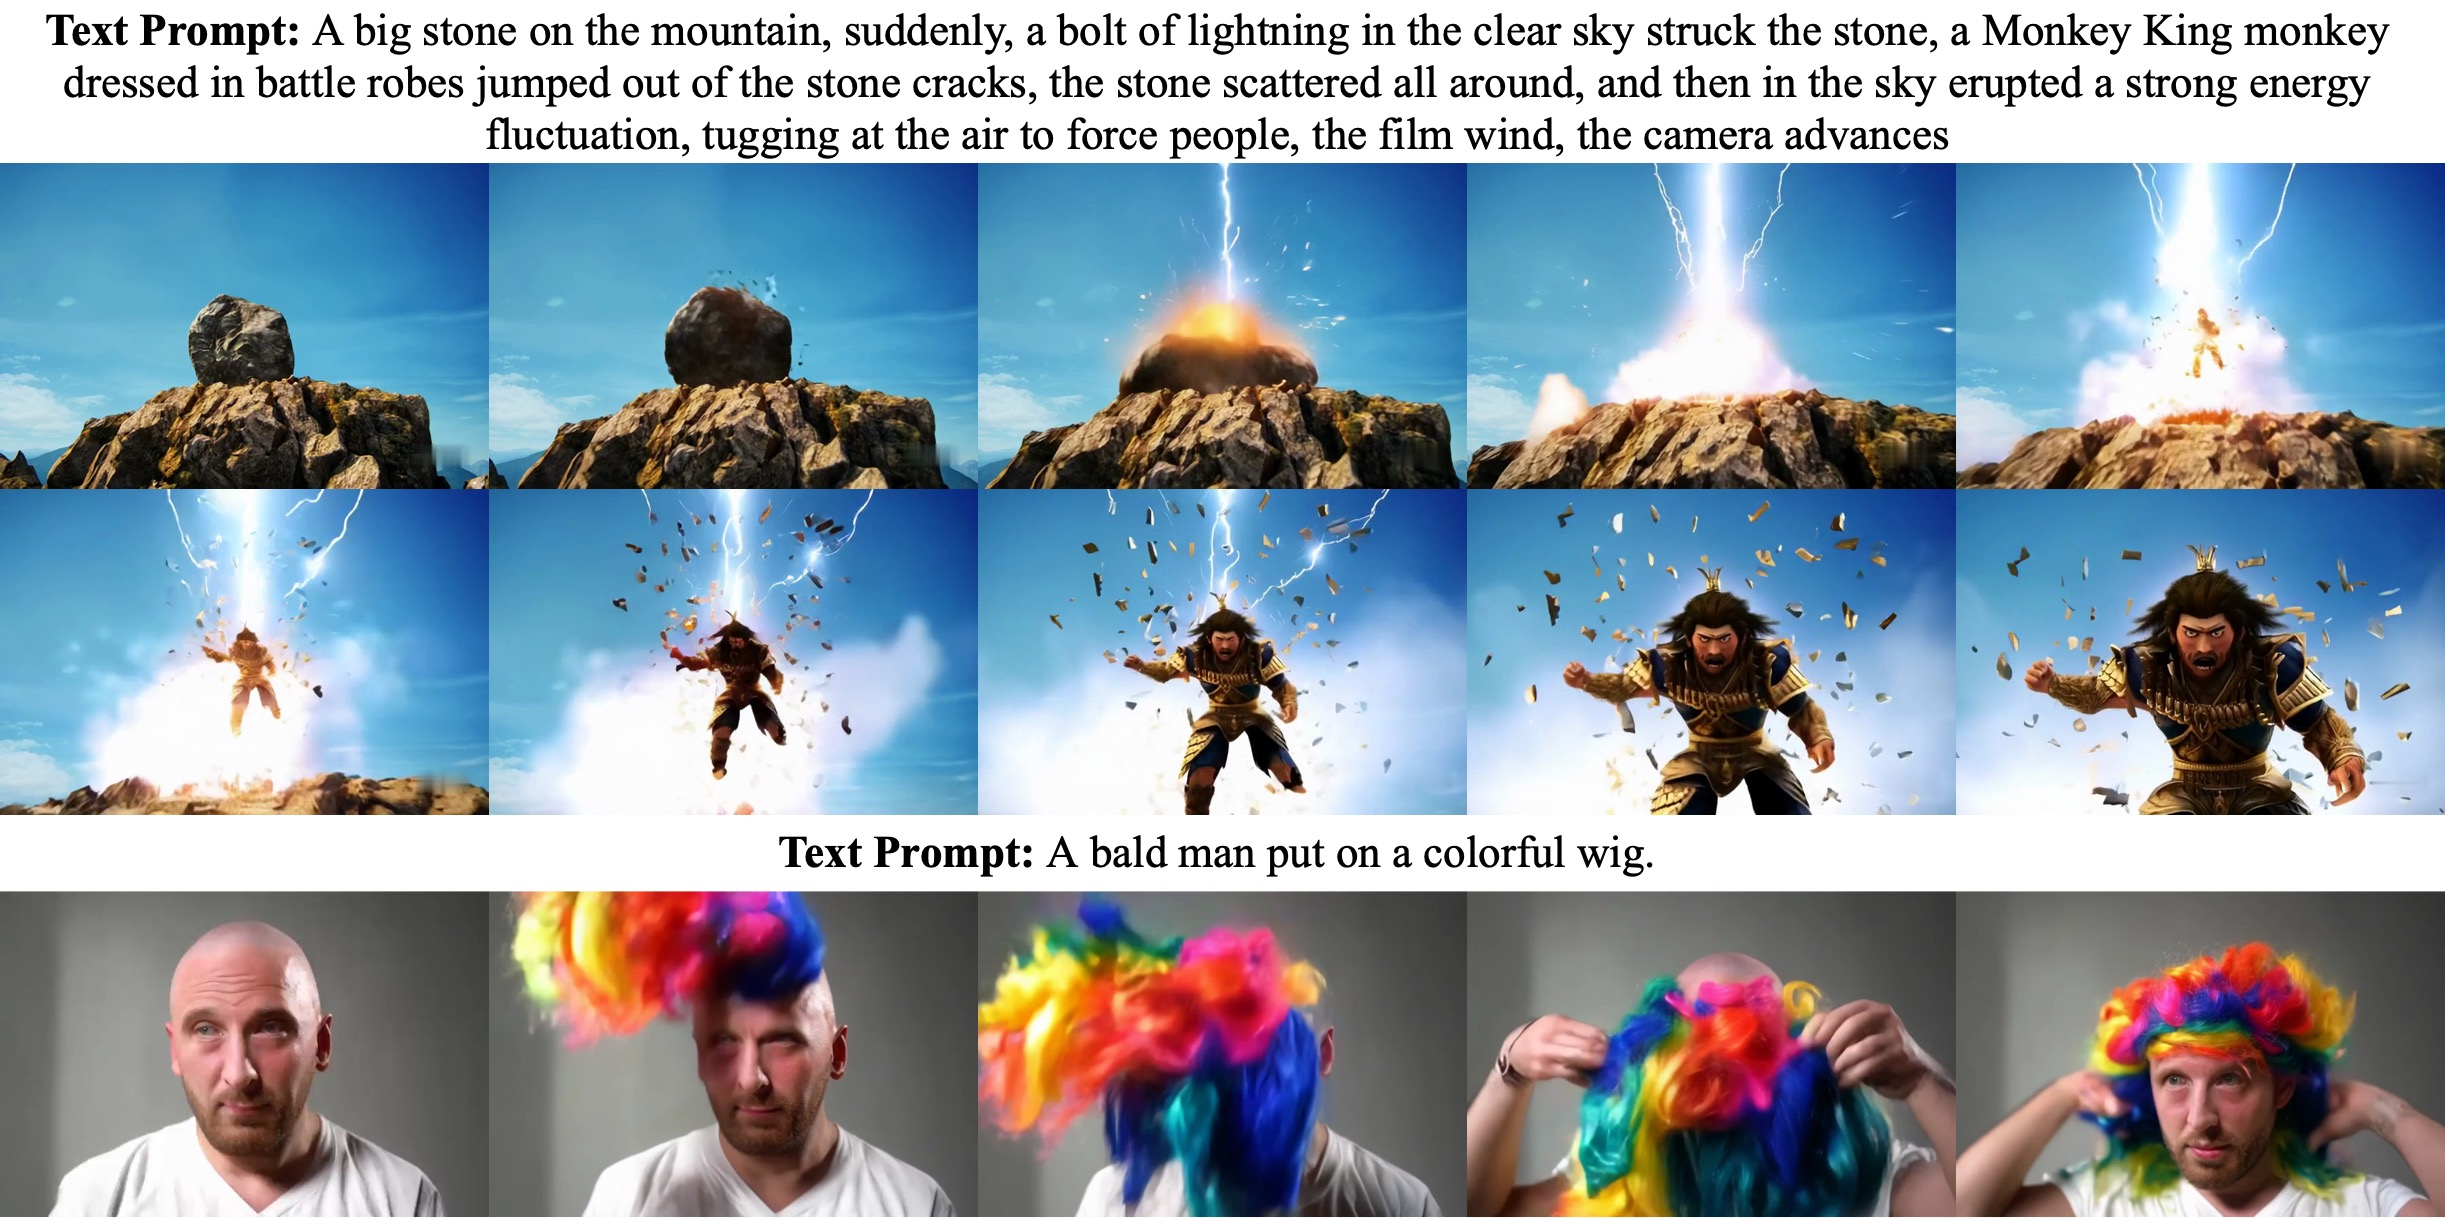
\includegraphics[width=\textwidth]{images/front.jpg}
\caption{
CogVideoX can generate long-duration, high-resolution videos with coherent actions and rich semantics.}
\label{fig:exampleImage}
\end{figure}

\begin{abstract}
%  Previous video generation models often had limited movement and short durations, making it difficult to generate videos with coherent narratives based on text. We propose several designs to address these issues and, train the CogVideoX., 
% To efficently model video data, we propose to levearge a 3D Variational Autoencoder (VAE) to compress videos along both spatial and temporal dimensions. 
% To improve the text-video alignment, we propose an expert transformer with the expert adaptive LayerNorm to facilitate the deep fusion between the two modalities. 
% By employing a progressive training technique, \model is adept at producing coherent, long-duration videos characterized by significant motions. 
% In addition, we develop an effective text-video data processing pipeline that includes various data preprocessing strategies and a video captioning method. 
% It significantly helps enhance the performance of \model, improving both generation quality and semantic alignment. 
% We introduce \model, large-scale diffusion transformer models designed for generating videos based on text prompts.

% Results show that \model demonstrates state-of-the-art performance across both multiple machine metrics and human evaluations. 
% The model weights of both the 3D Causal VAE and \model are publicly available at \anonymous.
%\url{https://github.com/THUDM/CogVideo}. 
% and \url{https://huggingfaces.co/THUDM/CogVideoX}. 

% Previous video generation models often had limited movement and short durations, making it difficult to generate videos with coherent narratives based on text. We propose several designs to address these issues and, introduce \model, large-scale diffusion transformer models which can generate 768$\times$ 1360 at 16 fps, 10 seconds videos based on text prompts. 
% First, we propose to levearge a 3D Variational Autoencoder (VAE) to compress videos along both spatial and temporal dimensions. Second, to improve the text-video alignment, we propose an expert transformer with the expert adaptive LayerNorm to facilitate the deep fusion between the two modalities. Third, by employing a progressive training and multi-resolution frame pack technique, \model is adept at producing coherent, long-duration, different shape videos characterized by significant motions. 
% In addition, we develop an effective text-video data processing pipeline that includes various data preprocessing strategies and a video captioning method. 
% It significantly helps enhance the performance of \model, improving both generation quality and semantic alignment. 
% Results show that \model demonstrates state-of-the-art performance across both multiple machine metrics and human evaluations. 
% The model weights of both the 3D Causal VAE and \model are publicly available at \anonymous.

We present \model, a large-scale text-to-video generation model based on diffusion transformer, which can generate 10-second continuous videos aligned with text prompt, with a frame rate of 16 fps and resolution of 768$\times$ 1360 pixels. 
Previous video generation models often had limited movement and short durations, and is difficult to generate videos with coherent narratives based on text. We propose several designs to address these issues. 
First, we propose a 3D Variational Autoencoder (VAE) to compress videos along both spatial and temporal dimensions, to improve both compression rate and video fidelity. Second, to improve the text-video alignment, we propose an expert transformer with the expert adaptive LayerNorm to facilitate the deep fusion between the two modalities. Third, by employing a progressive training and multi-resolution frame pack technique, \model is adept at producing coherent, long-duration, different shape videos characterized by significant motions. 
In addition, we develop an effective text-video data processing pipeline that includes various data preprocessing strategies and a video captioning method,
% . It significantly helps enhance the performance of \model, improving both generation quality and semantic alignment. 
greatly contributing to the generation quality and semantic alignment. 
Results show that \model demonstrates state-of-the-art performance across both multiple machine metrics and human evaluations. 
% The model weights of the 3D Causal VAE, the video caption model, and CogVideoX are open-source.
The model weight of both 3D Causal VAE, Video caption model and \model are publicly available at \href{https://github.com/THUDM/CogVideo}{https://github.com/THUDM/CogVideo}.


\end{abstract}


\section{Introduction}
Despite the well-recognized importance of training data in advancing the capabilities of large language models (LLMs)~\cite{brown2020language,kaplan2020scaling,Razeghi2022ImpactOP}, there is no agreed-upon mechanisms for crediting or compensating data providers. As LLMs are increasingly integrated into our society and economy, the absence of such mechanisms has aggravated a tension between data and model providers, exemplified by recent legal challenges involving major tech companies~\cite{jlversusalphabet,metz2022lawsuit}. In this atmosphere, data valuation, which quantifies the contribution of each training data to the model output, has been discussed as a potential technical solution for tackling these societal issues~\cite{fernandez2023data,ghorbani2019data,huang2023citation,jia2019towards,worledge2023unifying,zhao2023addressing}. 

At a high level, most data valuation algorithms interpret the model output as a coalition of its training data, and evaluate the contribution of each example based on its influence on the model output when included or excluded from the training dataset~\cite{ghorbani2019data,ilyas2022datamodels,koh2017understanding,kwon2021beta}. If an inclusion of a specific training example consistently improves model performance, high value can be assigned to this example for its contribution. However, applying existing data valuation methods to recent LLMs and their vast training datasets has faced significant scalability challenges to date. For instance, sampling-based methods, such as the Shapley value~\cite{ghorbani2019data,kwon2021beta} or Datamodels~\cite{ilyas2022datamodels}, require retraining the model multiple times with varied combinations of data subsets to directly model the effect of in/excluding each data. Unfortunately, such repeated retraining is hardly affordable even for small models, let alone LLMs. To overcome this issue, gradient-based methods, including influence functions~\cite{koh2017understanding,park2023trak}, approximate the effect of data in/exclusion on the model output using gradient information without costly retraining. Even so, scaling gradient-based methods to LLMs is hindered by prohibitive compute and memory costs originating in the high-dimensional nature of the gradient.

Consequently, the main objective of this work is to bridge the gap in scaling existing data valuation methods to recent LLMs and their vast training datasets. Toward this goal, we focus on influence functions \cite{koh2017understanding,park2023trak}, a representative gradient-based data valuation method, and significantly improve its scalability with an efficient gradient projection algorithm. We visualize the proposed data valuation system in Figure~\ref{fig:diagram}, and detail our technical contributions below:

\begin{figure}
    \centering
    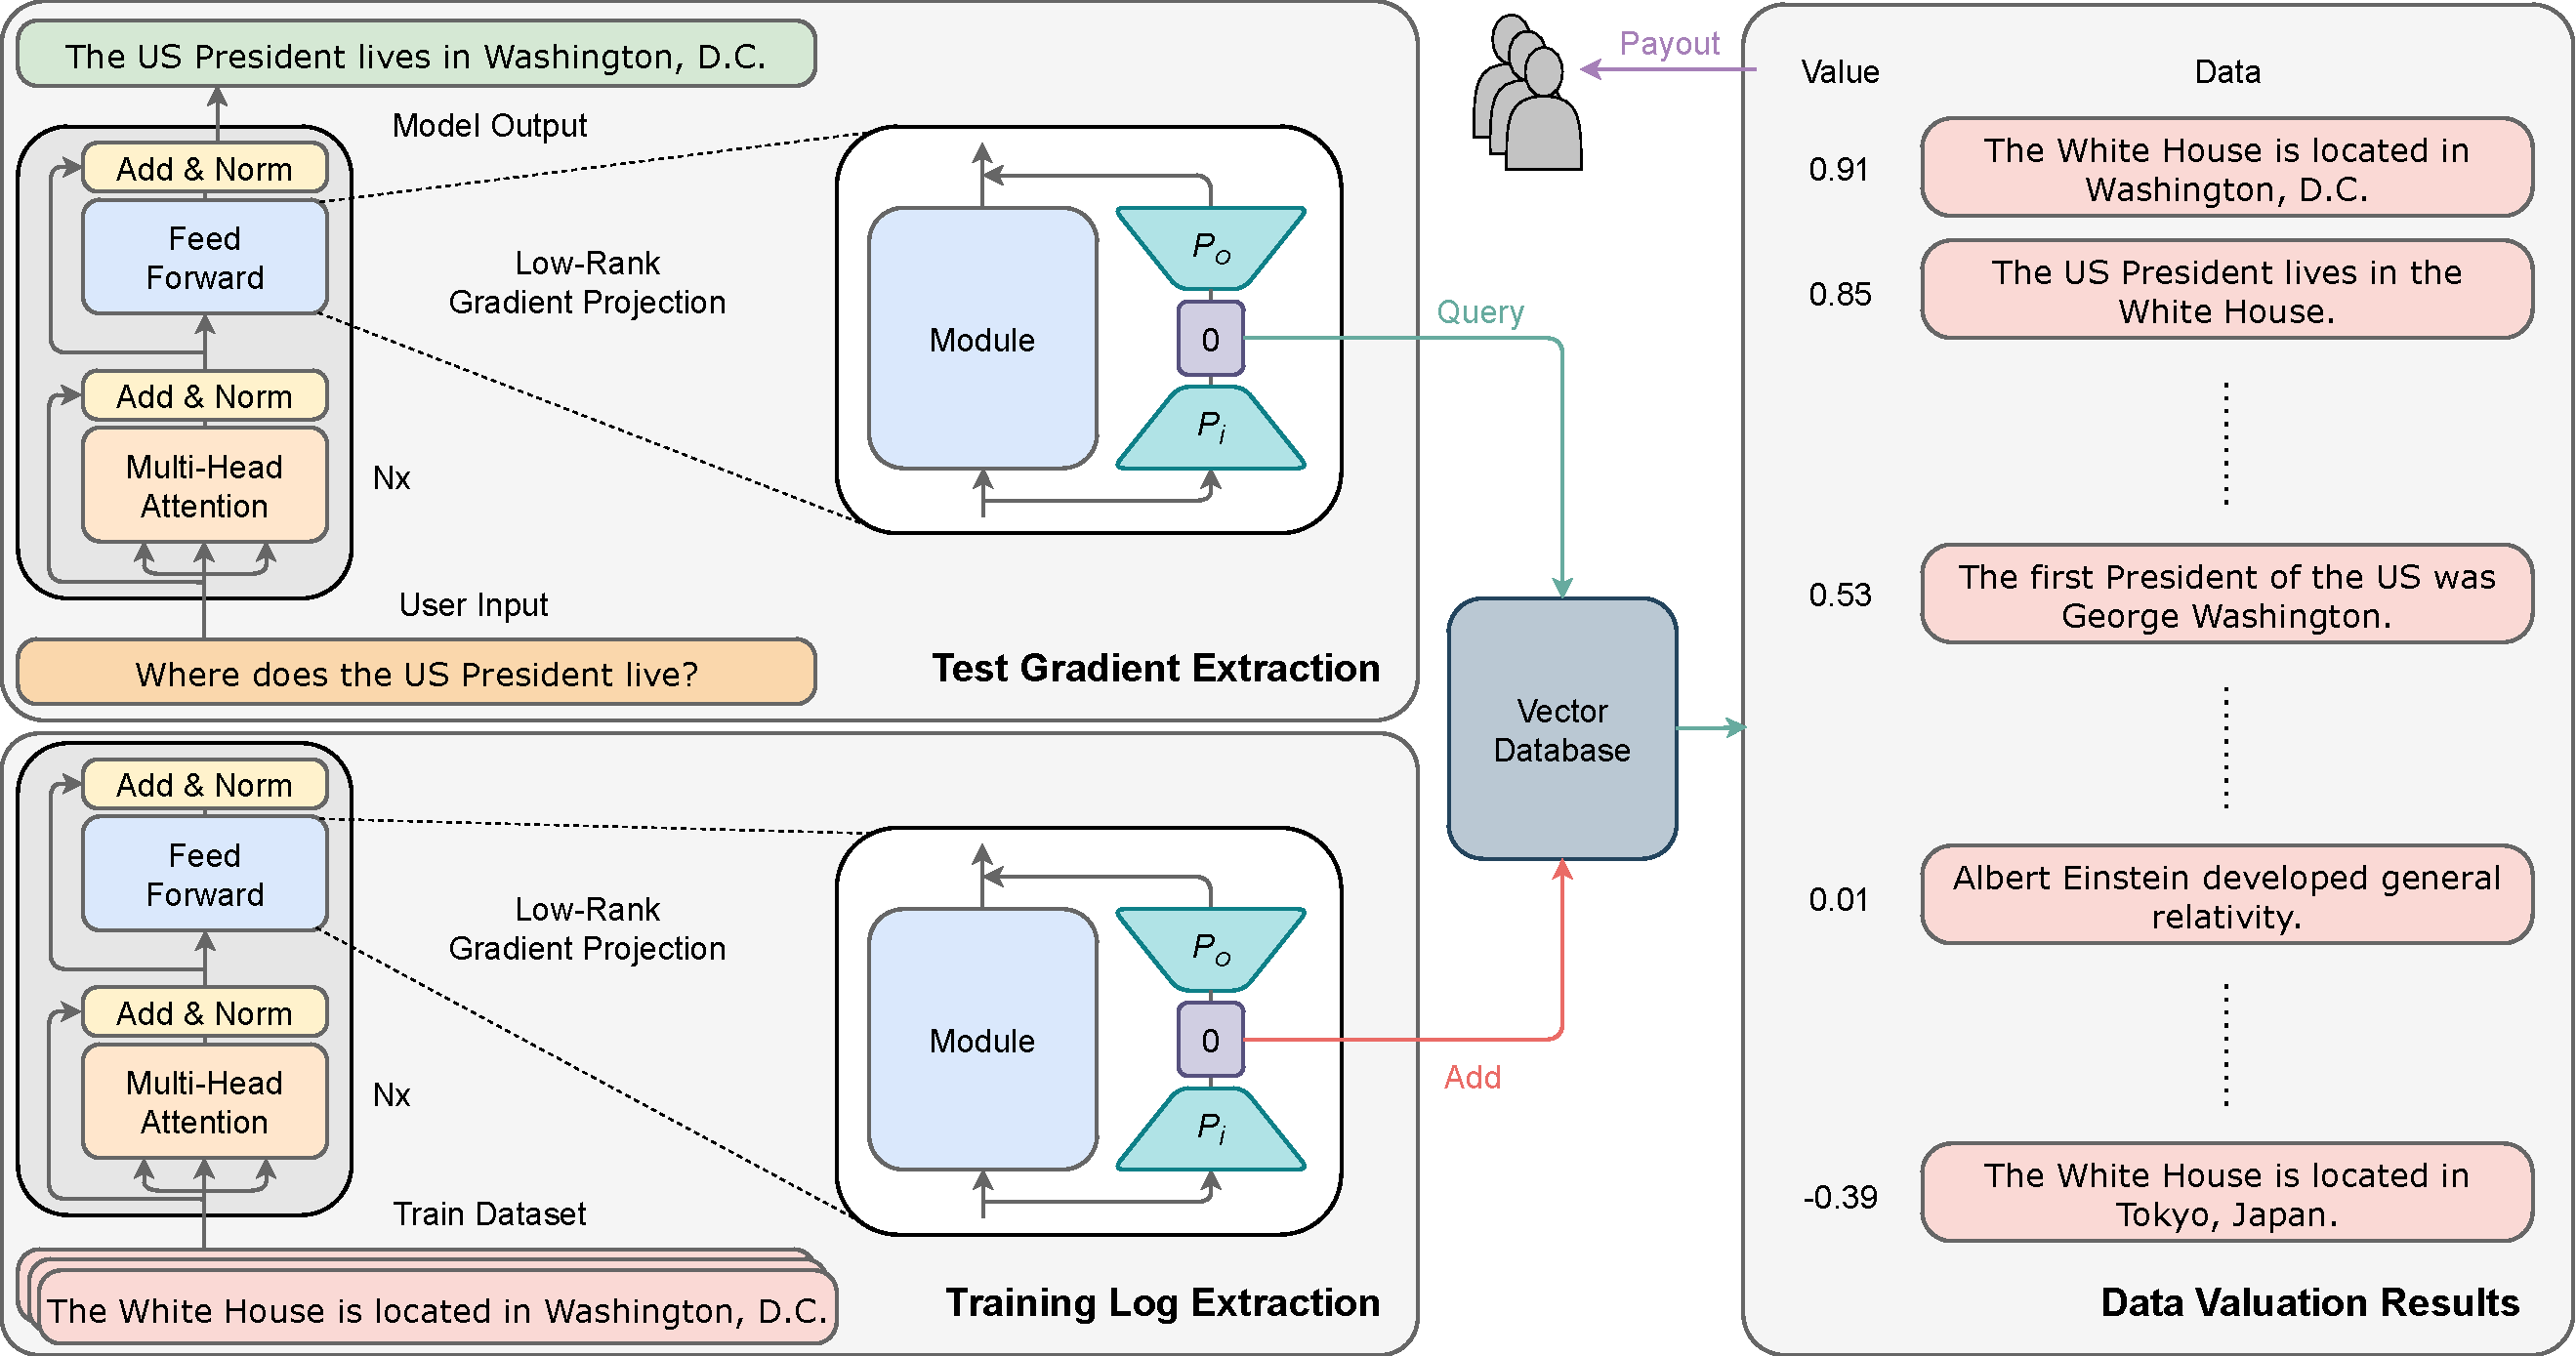
\includegraphics[width=0.94\textwidth]{figures/diagram_v7.pdf}
    \vskip -4pt
    \caption{Data valuation system architecture. \textbf{(Left Bottom)} We first extract the Hessian and gradients for all training data using efficient gradient projection \method\ and store them in a database. \textbf{(Left Top)} At test time, we similarly extract gradients and query the database. \textbf{(Right)} The database returns similarity scores with respect to training examples that can be used for data valuation/attribution.}
    \label{fig:diagram}
\end{figure}

\begin{itemize}[leftmargin=*,topsep=-2pt]
    \item Employing gradient structures in backpropagation, we develop a novel \textbf{lo}w-rank \textbf{gra}dient projection algorithm \method\ that improves space \& time complexity of gradient projection, a major scalability bottleneck in prior work~\cite{park2023trak,schioppa2022scaling}, from $O(nk)$ to $O(\sqrt{nk})$ where $n$ and $k$ are model and projection dimensions. Furthermore, \method\ directly computes projected gradients without materializing full gradients, enabling low GPU memory and high GPU utilization for improved efficiency. Lastly, we show that \method\ can be easily implemented with small add-on layers, similarly to LoRA~\cite{hu2021lora}.
    \item By interpreting a damping term in influence functions as a spectral gradient sparsification mechanism, we (1) offer a theoretical motivation of gradient projection approaches to influence functions and (2) derive a specialized PCA initialization scheme for \method.
    \item We introduce software named \software\ that (1) makes it \textit{simple} to convert existing training code into data valuation code, (2) is \textit{compatible} with various scalability tools and features in the LLM ecosystem, and (3) is \textit{extensible} to implement other data valuation or interpretability algorithms.
    \item In our data valuation experiments, \method\ demonstrates competitive accuracy against more costly baselines, while showing up to 6,500$\times$ increase in throughput and 5$\times$ reduction in GPU memory, when applied to Llama3-8B-Instruct~\cite{llama3modelcard} and the 1B-token dataset, compared to EKFAC influence \cite{grosse2023studying}, the state-of-the-art and only runnable baseline at this scale. We also observe that most valuable data identified by \method\ generally share qualitative similarities with the queried LLM output.
\end{itemize}
\subsection{3D Variational Auto-encoder Design}\label{3dVAE}

Similar to previous work~\cite{polyak2024movie,yang2024cogvideox}, we train a 3DVAE to compress pixel-space videos and images into a compact latent space. To handle both videos and images, we adopt CausalConv3D~\cite{yu2023language}. For a video of shape $(T+1) \times 3 \times H \times W$, our 3DVAE compresses it into latent features with shape $(\frac{T}{c_t} + 1) \times C \times (\frac{H}{c_s}) \times (\frac{W}{c_s})$. In our implementation, $c_t=4$, $c_s=8$, and $C=16$. This compression significantly reduces the number of tokens for the subsequent diffusion transformer model, allowing us to train videos at the original resolution and frame rate. The model structure is illustrated in Figure \ref{fig:vae-model-arch}.

\begin{figure}[t]
    \centering
    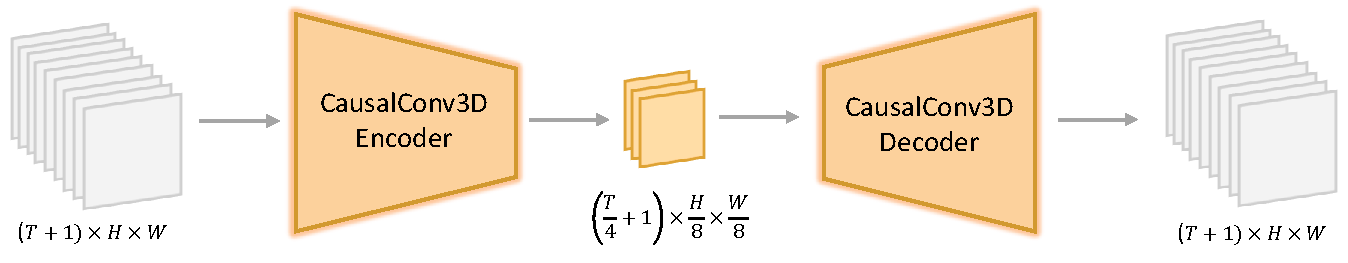
\includegraphics[width=0.95\linewidth]{figures/vae-model-arch.pdf}
    \caption{ The architecture of our 3DVAE.}
    \label{fig:vae-model-arch}
\end{figure}

\subsubsection{Training}
In contrast to most previous work \cite{polyak2024movie,chen2024od,zhou2024allegro}, we do not rely on a pre-trained image VAE for parameter initialization; instead, we train our model from scratch. 
To balance the reconstruction quality of videos and images, we mix video and image data at a ratio of $4:1$. Besides the routinely used $L_1$ reconstruction loss and KL loss $L_{kl}$, we also incorporate perceptual loss $L_{lpips}$ and GAN adversarial loss $L_{adv}$ \cite{esser2021taming} to enhance the reconstruction quality. The complete loss function is shown in Equation \ref{eq:vae-loss}.

\begin{equation}
    \label{eq:vae-loss}
    \text{Loss} = L_{1} + 0.1 L_{lpips} + 0.05 L_{adv} + 10^{-6} L_{kl}
\end{equation}

During training, we employ a curriculum learning strategy, gradually training from low-resolution short video to high-resolution long video. To improve the reconstruction of high-motion videos, we randomly choose a sampling interval from the range $1 \sim 8$ to sample frames evenly across video clips.

\subsubsection{Inference}
Encoding and decoding high-resolution long videos on a single GPU can lead to out-of-memory (OOM) errors. To address this, we use a spatial-temporal tiling strategy, splitting the input video into overlapping tiles along the spatial and temporal dimensions. Each tile is encoded/decoded separately, and the outputs are stitched together. For the overlapping regions, we utilize a linear combination for blending. This tiling strategy allows us to encode/decode videos in arbitrary resolutions and durations on a single GPU.

We observed that directly using the tiling strategy during inference can result in visible artifacts due to inconsistencies between training and inference. To solve this, we introduce an additional finetuning phase where the tiling strategy is randomly enabled/disabled during training. This ensures the model is compatible with both tiling and non-tiling strategies, maintaining consistency between training and inference. 

\begin{figure}[ht]
    \centering
    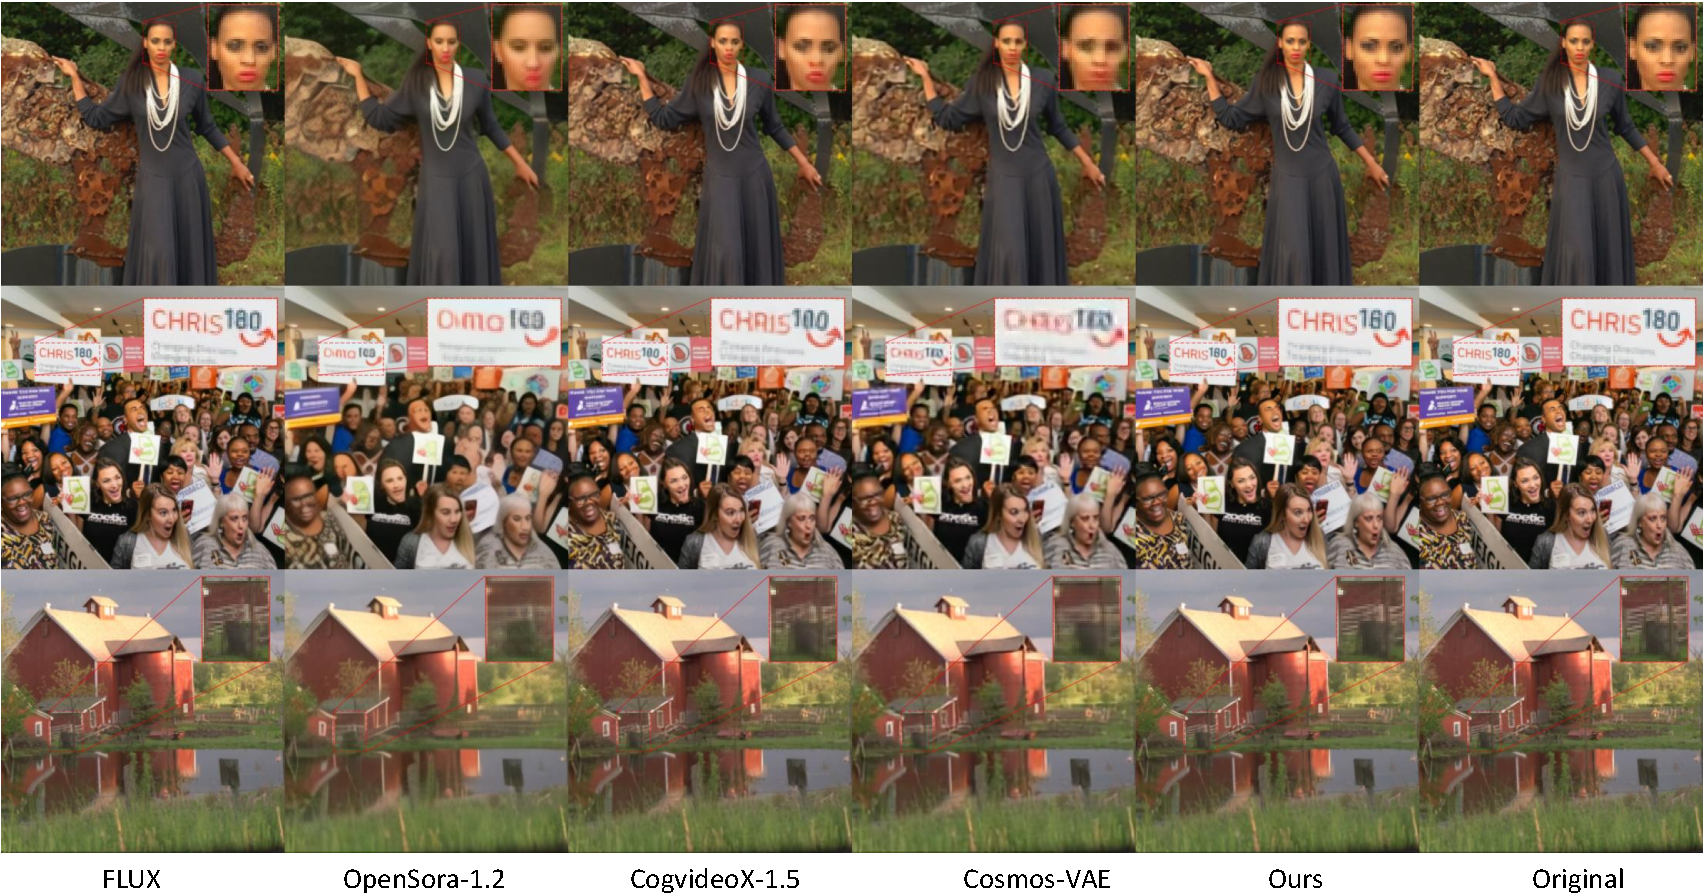
\includegraphics[width=\linewidth]{figures/vae-sota-cmp.pdf}
    \caption{VAE reconstruction case comparison.}
    \label{fig:vae-sota-cmp}
\end{figure}

Table \ref{tab:sota_vae} compares our VAE with open-source state-of-the-art VAEs. On video data, our VAE demonstrates a significantly higher PSNR compared to other video VAEs. On images, our performance surpasses both video VAEs and image VAE. Figure \ref{fig:vae-sota-cmp} shows several cases at $256 \times 256$ resolution. Our VAE demonstrates significant advantages in text, small faces, and complex textures.
%Table \ref{tab:sota_vae} compares our VAE with open-source state-of-the-art VAEs. On video data, our VAE demonstrates a significantly higher PSNR compared to other video VAEs, achieving performance comparable to frame-wise image VAE while maintaining a 4x higher temporal compression. On images, our PSNR not only surpasses that of other video VAEs but also exceeds that of image VAE. Figure \ref{fig:vae-sota-cmp} shows several cases at $256 \times 256$ resolution. It is evident that our VAE demonstrates significant advantages in  text, small faces, and complex textures.


\begin{table*}[ht]
\renewcommand{\arraystretch}{1.2}
\small
\centering  
\caption{VAE reconstruction metrics comparison.}
\begin{tabular}{lcccc}
\toprule
\multirow{2}{*}{Model} & Downsample  & \multirow{2}{*}{$|z|$} & ImageNet (256$\times$256)
& MCL-JCV (33$\times$360$\times$640) \\
& Factor & & PSNR$\uparrow$ & PSNR$\uparrow$ \\
\midrule
%FLUX-VAE~\cite{FLUX}                   & $1 \times 8 \times 8$ & 16 & 32.70 & 37.87 \\
FLUX-VAE~\cite{FLUX}                   & $1 \times 8 \times 8$ & 16 & 32.70 & - \\
\midrule
OpenSora-1.2~\cite{opensora}           & $4 \times 8 \times 8$ & 4  & 28.11 & 30.15 \\
CogvideoX-1.5~\cite{yang2024cogvideox} & $4 \times 8 \times 8$ & 16 & 31.73 & 33.22 \\
Cosmos-VAE~\cite{cosmos}               & $4 \times 8 \times 8$ & 16 & 30.07 & 32.76 \\
Ours                                   & $4 \times 8 \times 8$ & 16 & 33.14 & 35.39 \\
\bottomrule
\end{tabular}
\label{tab:sota_vae}
\end{table*}

\begin{figure}[h]
\begin{center}
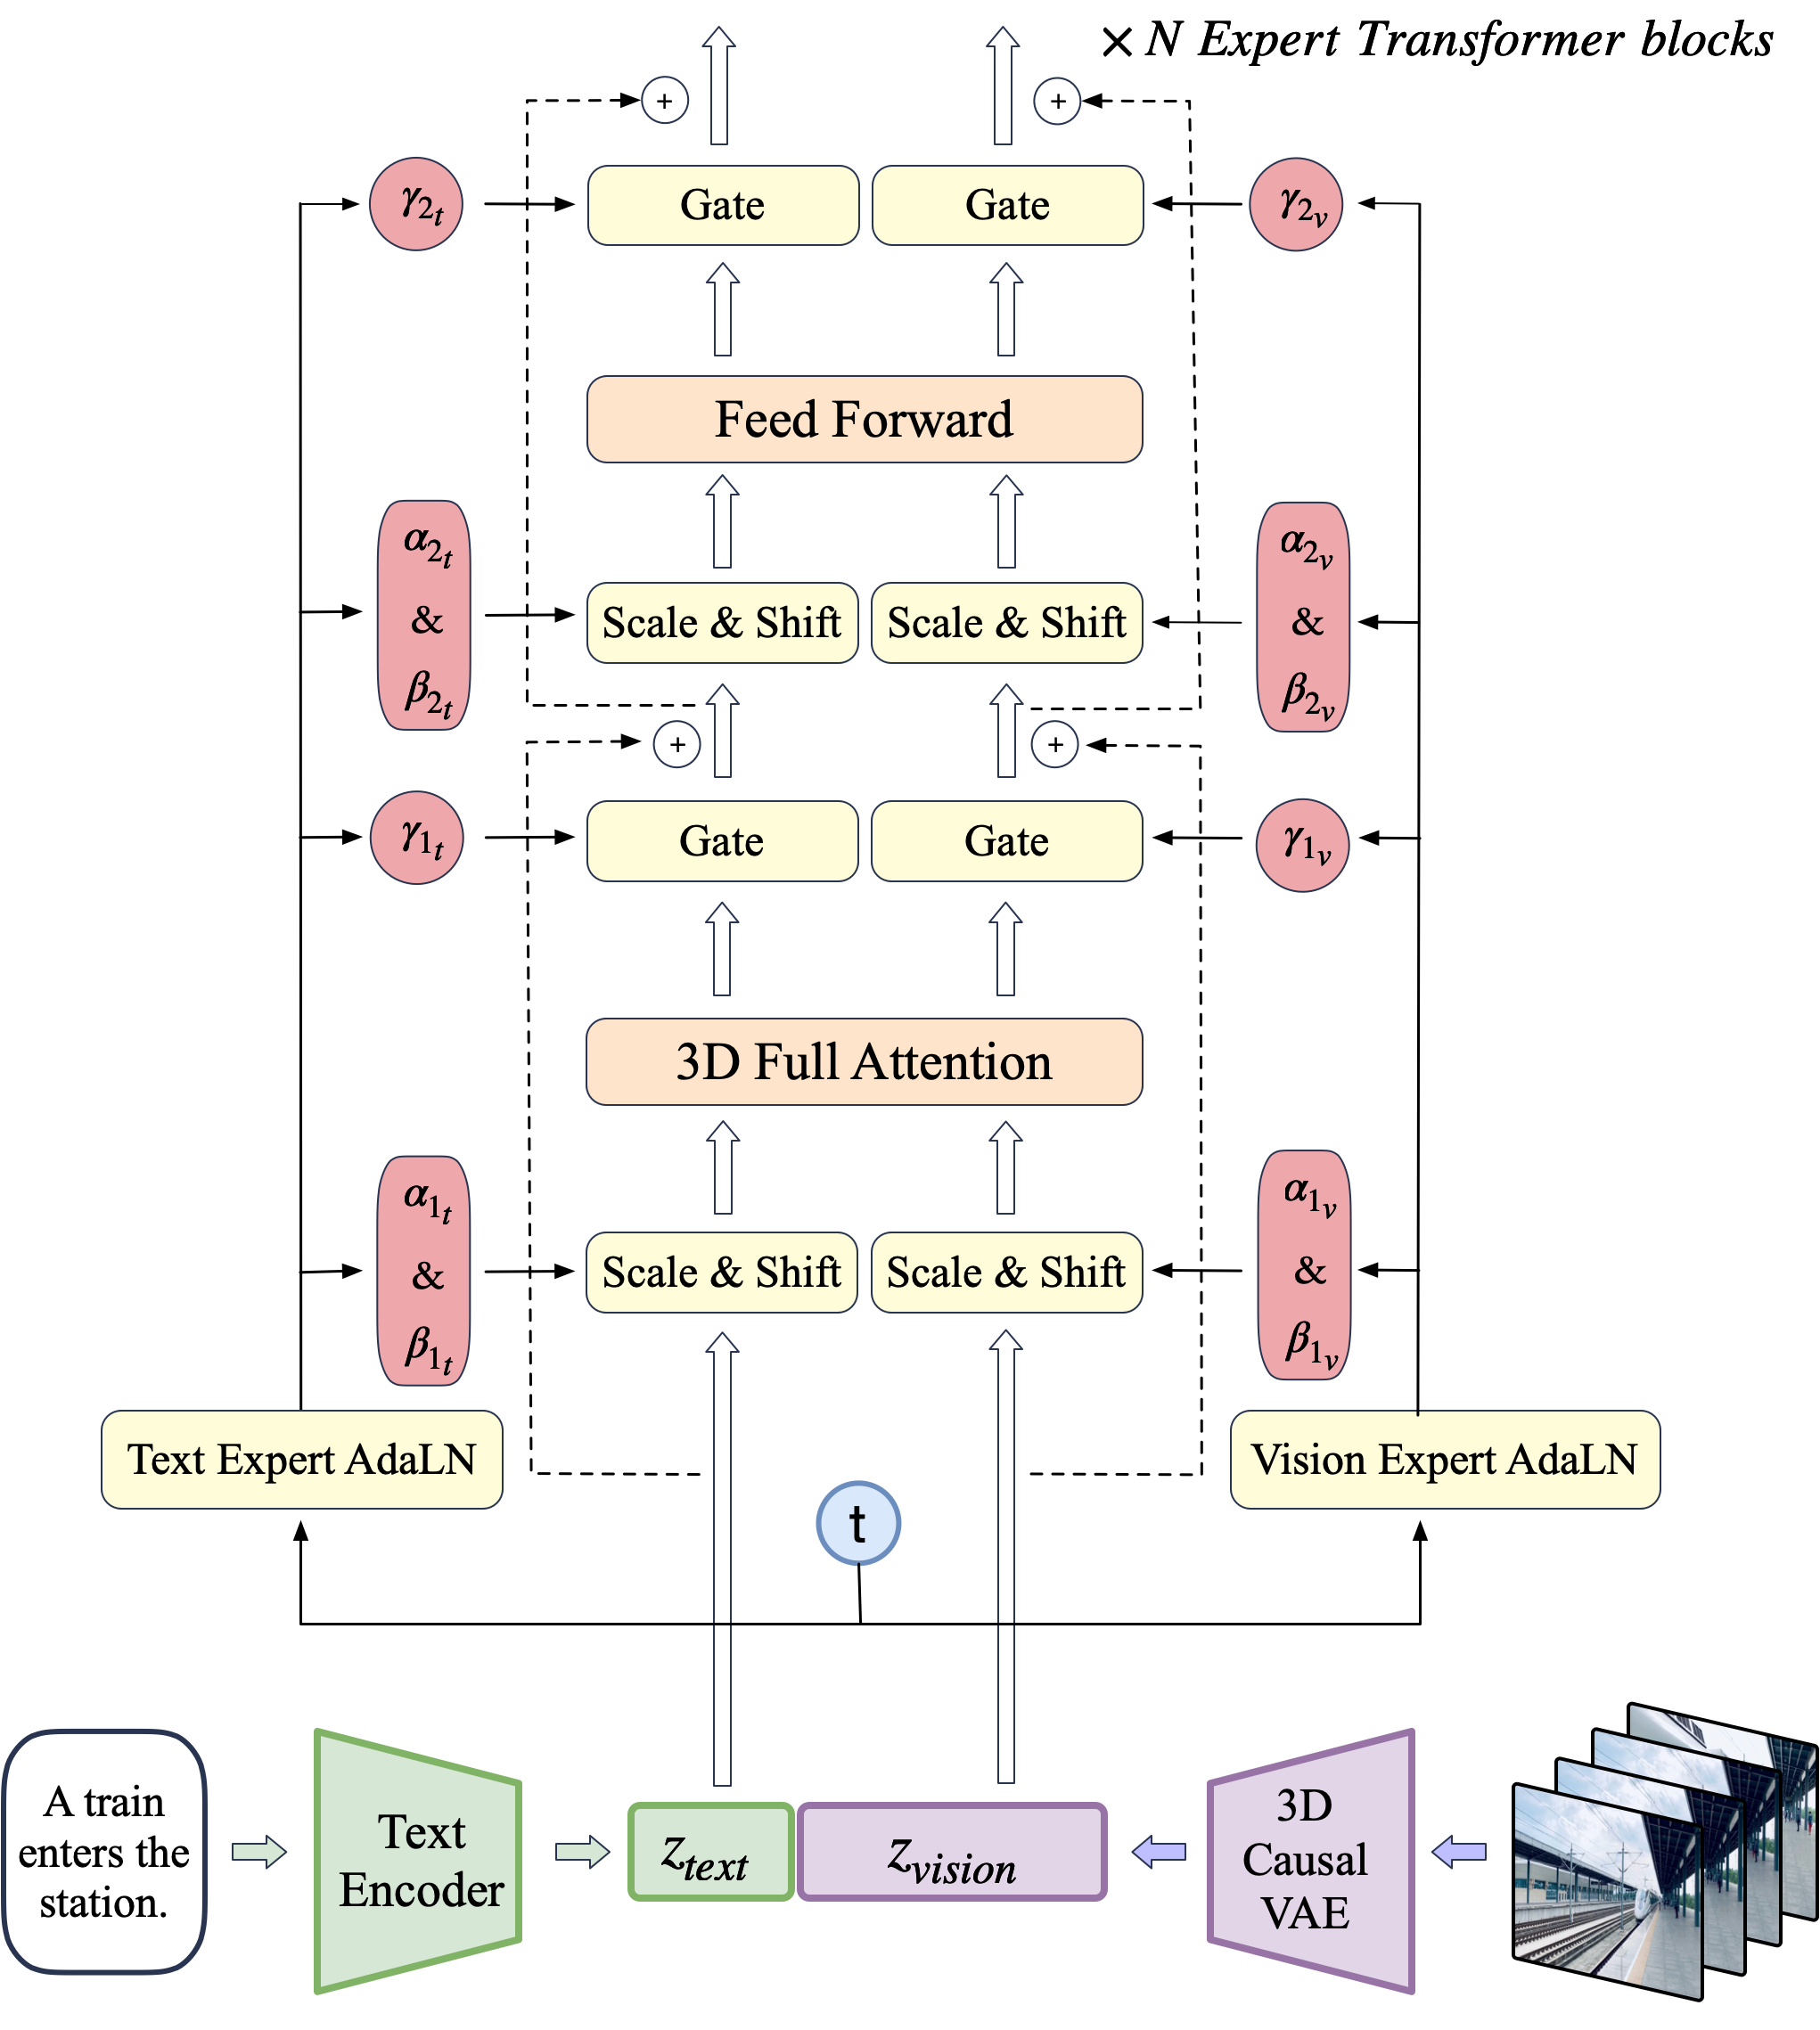
\includegraphics[width=0.7\linewidth]{images/transformer.png}
\end{center}
\caption{\textbf{Our model architecture.} }
\label{fig:model}
\end{figure}

\subsection{Expert Transformer}\label{sec:expert-transformer}

\paragraph{Patchify}
After being encoded into latent vectors of shape $T \times H \times W \times C$ by the 3D causal VAE, the video latents are patchified  along the spatial dimensions, resulting sequence $z_{\text{vision}}$ of length $T\cdot \frac{H}{p} \cdot \frac{W}{p}$. 
% VAE encodes the video into a latent vector of shape $T \times H \times W \times C$. Then we patchify the latent along the spatial dimensions, generating sequence $z_{vision}$ of length $T\cdot \frac{H}{p} \cdot \frac{W}{p}$. 
We do not patchify along the temporal dimension in order to enable joint training of images and videos.

\paragraph{3D-RoPE}
Rotary Position Embedding (RoPE)~\citep{su2024roformer} is a relative positional encoding that has been demonstrated to capture inter-token relationships effectively in LLMs, particularly excelling in modeling long sequences. To adapt to video data, we extend RoPE to 3D. 
Each latent in the video tensor can be represented by a 3D coordinate $(x, y, t)$.
We independently apply 1D-RoPE to each dimension of the coordinates, each occupies $3/8$, $3/8$, $2/8$ of the hidden states's channel. The resultsing encoding are then concatenate along the channel dimension to obtain the final 3D-RoPE encoding.

\paragraph{Expert Transformer Block}
We concatenate the embeddings of both text and video at the input stage to better align visual and semantic information. However, the feature spaces of these two modalities differ significantly, and their embeddings may even have different numerical scales. To better process them within the same sequence, we employ Expert Adaptive Layernorm to handle each modality independently.
As shown in Figure~\ref{fig:model}, following DiT~\citep{peebles2023scalable}, we use the timestep $t$ of the diffusion process as the input to the modulation module. 
Then, the Vision Expert Adaptive Layernorm and Text Expert Adaptive Layernorm independently apply this modulation mechanism to the vision hidden states and text hidden states respectively. This method promotes the alignment of feature spaces across two modalities while minimizing additional parameters.



\paragraph{3D Full Attention}
Previous works \citep{singer2022make, guo2023animatediff} often employ separated spatial and temporal attention to reduce computational complexity and facilitate fine-tuning from text-to-image models. However, as illustrated in Figure~\ref{fig:attention}, this separated attention approach requires extensive implicit transmission of visual information, significantly increasing the learning complexity and making it challenging to maintain the consistency of large-movement objects. Considering the great success of long-context training in LLMs and the efficiency of FlashAttention, we propose a 3D text-video hybrid attention mechanism. This mechanism not only achieves better results but can also be easily adapted to various parallel acceleration methods. 


\begin{wrapfigure}{r}{0.5\textwidth}
\centering
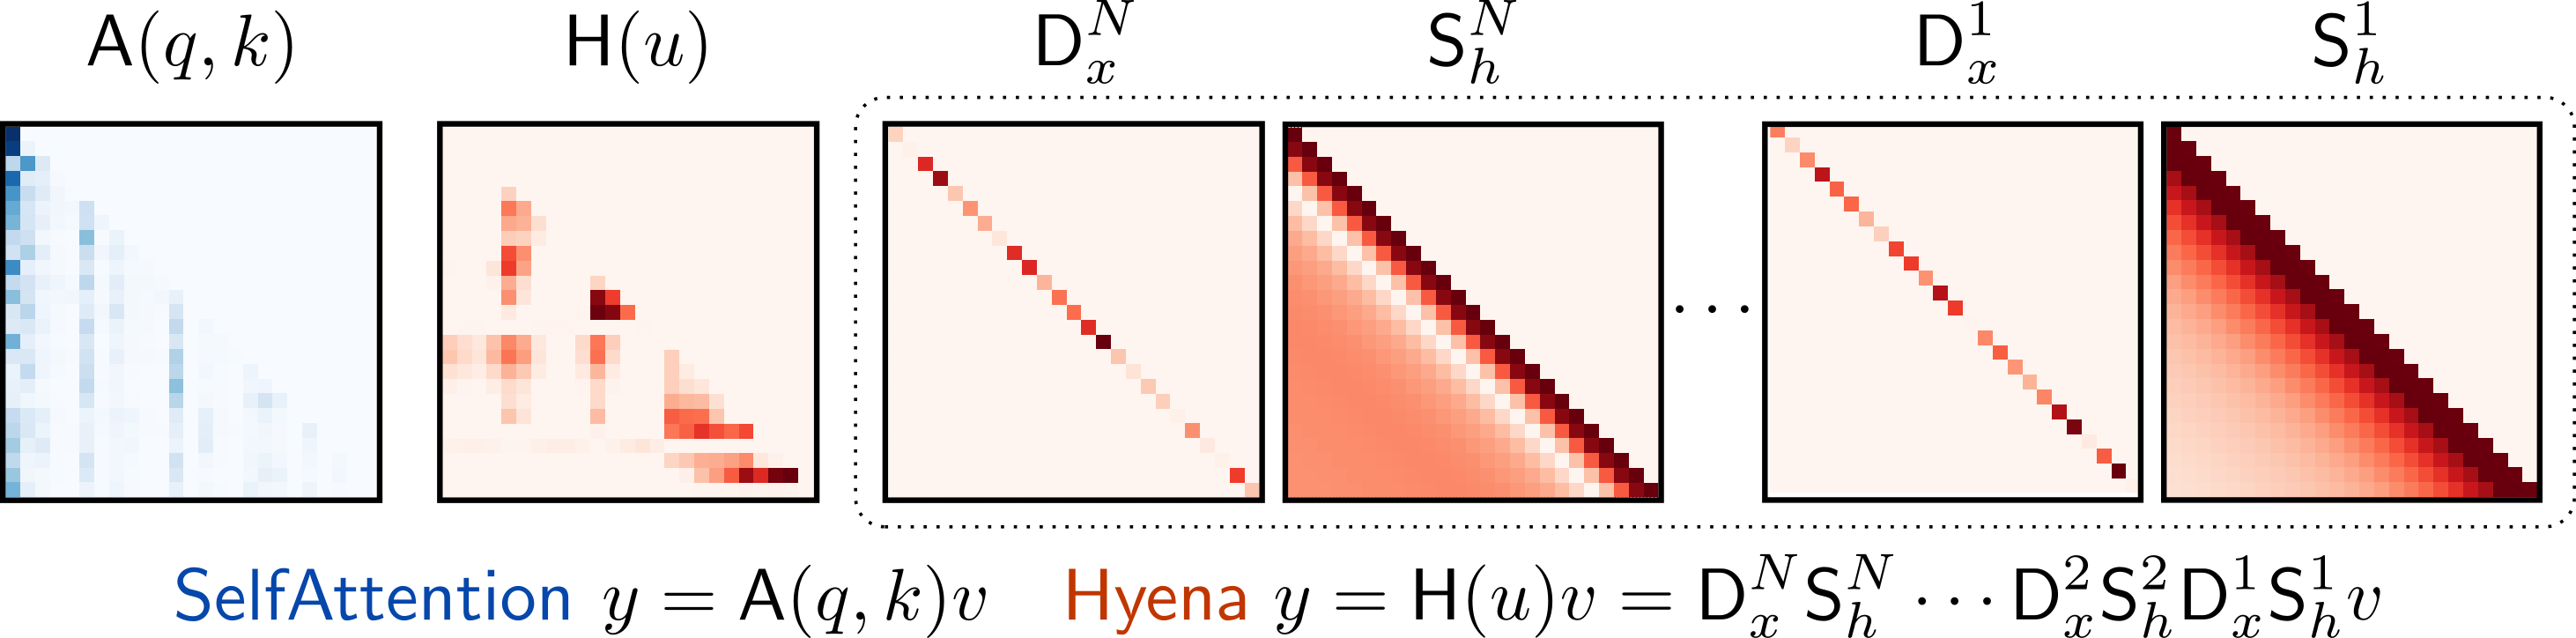
\includegraphics[width=\linewidth]{images/attention.png}
\caption{The separated spatial and temporal attention makes it challenging to  handle the large motion between adjacent frames. In the figure, the head of the person in frame $i+1$ cannot directly attend to the head in the frame $i$. Instead, visual information can only be implicitly transmitted through other background patches. This can lead to inconsistency issues in the generated videos.}
\label{fig:attention}
\vspace{-10mm}
\end{wrapfigure}




\section{Training}

\begin{figure}[ht]
\begin{center}
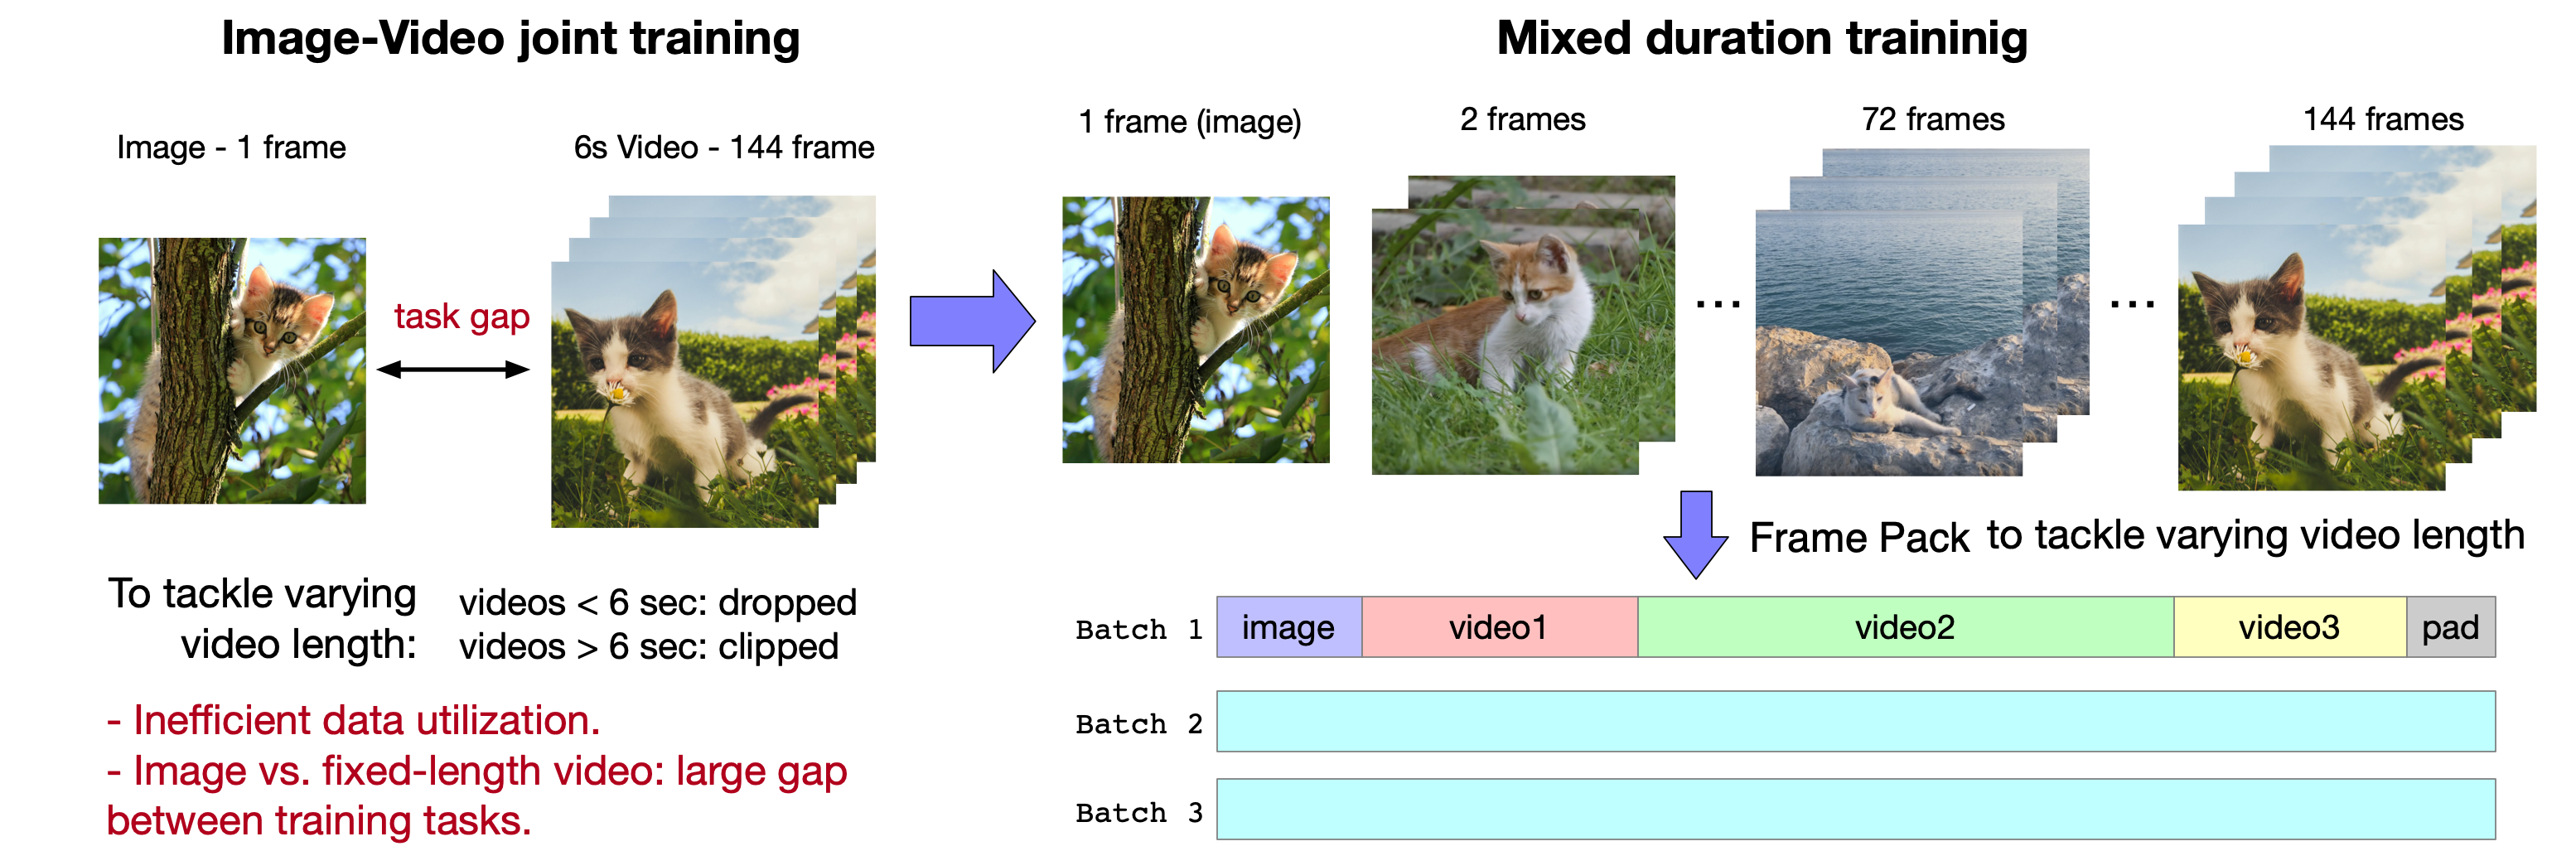
\includegraphics[width=\linewidth]{images/CogVideoX.png}
\end{center}
\caption{
The diagram of Mixed duration training and Frame Pack. To fully utilize the data and enhance the model's generalization capability, we train with videos of different durations within the same batch.}
\label{fig:framepack}
\end{figure}

\subsection{Setting}
We mixed images and videos during training, treating each image as a single-frame video. Additionally, we employed progressive training from the resolution perspective. For the diffusion setting, we adopt v-prediction~\citep{salimans2022progressive} and zero SNR~\citep{lin2024common}, following the noise schedule used in LDM~\citep{rombach2022high}.
During diffusion training for timestep sampling, we also employed an explicit uniform timestep sampling method, which benefits stable training. 

\subsection{Frame Pack}
Previous video model training methods often involved jointly training images and fixed frames videos. However, this approach led to two major problems: 1. There is a significant gap between the two input types using bidirectional attention, with images having 1 frame while videos having dozens of frames. We observed that models trained this way tend to diverge into two generative modes based on the token number and do not generalize well. 2. For training with a fixed duration, we need to discard short videos and truncate long videos, which prevents full utilization of the videos of varying frames.

To address these issues, we chose mixed-duration training, which means training videos of different lengths together. However, inconsistent data shapes within the batch make training difficult. Inspired by Patch'n Pack \citep{dehghani2024patch}, we place videos of different lengths into the same batch to ensure consistent shapes within each batch, a method we refer to as Frame Pack. 

\subsection{resolution prograssive training}
Our training pipeline is divided into three stages: low-resolution training, high-resolution training, and high-quality video fine-tuning. Similar to images, internet videos also include a significant amount of low-resolution videos. Prograssive training can effectively utilize various resolution videos. 
Moreover, training at low resolution initially can equip the model with coarse-grained modeling capabilities, followed by high-resolution training to enhance the model's ability to capture fine details. Compared to direct high-resolution training, staged training can reduce the overall training time.
\begin{figure}[h]
\begin{center}
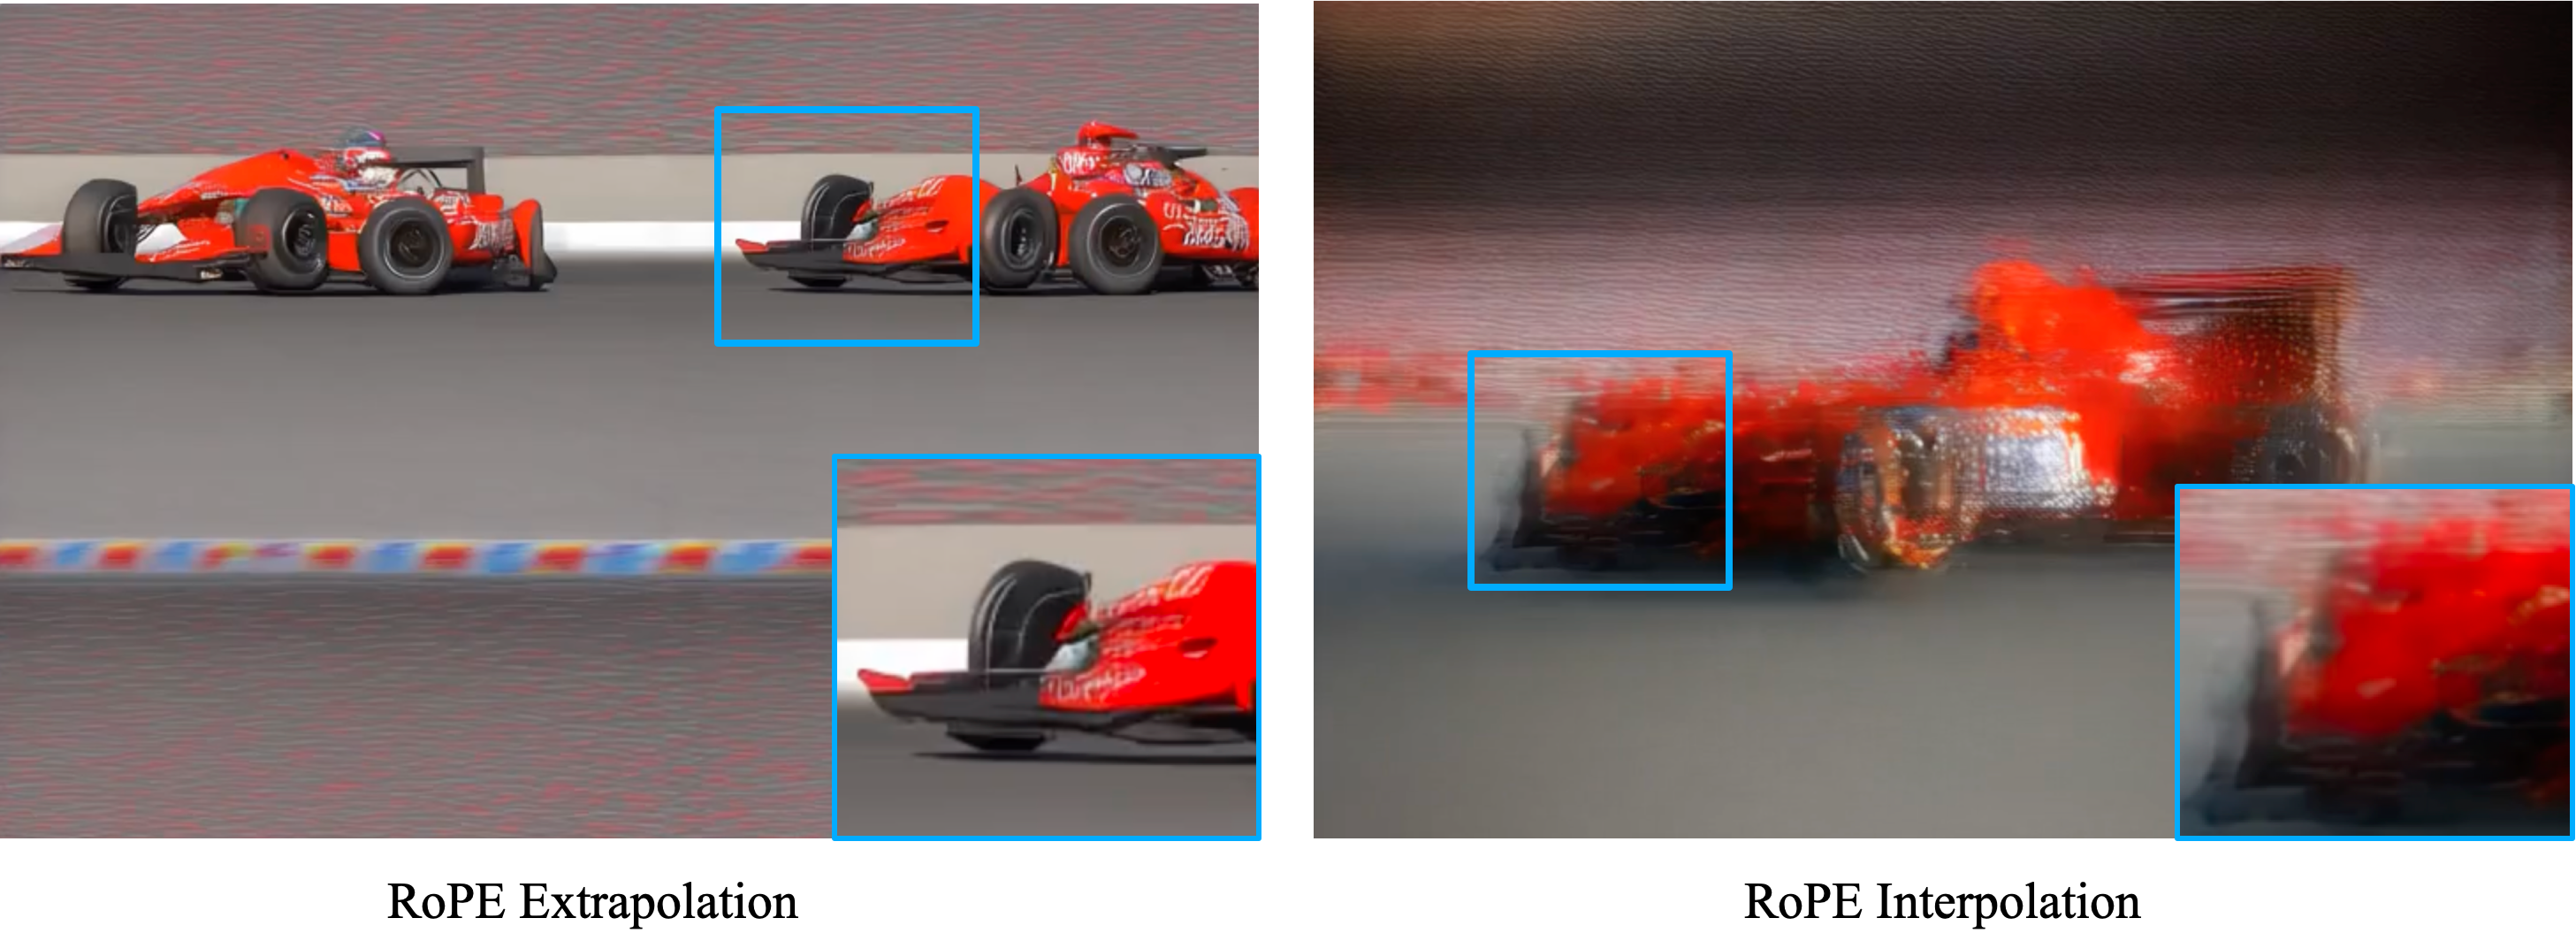
\includegraphics[width=0.9\linewidth]{images/ive.png}
\end{center}
\caption{We compared the initial generation states of extrapolation and interpolation when increasing resolution with RoPE encoding. Extrapolation tends to generate multiple small, clear, and repetitive images, while interpolation generates a blurry large image.}
\label{fig:ive}
\end{figure}

\paragraph{Extrapolation of position code}
When adapting low-resolution position encoding to high-resolution, we consider two different methods: interpolation and extrapolation. We show the effects of two methods in Figure~\ref{fig:ive}. Interpolation tens to preserve global information more effectively, whereas the extrapolation better retains local details. Given that RoPE is a relative position encoding, We chose the extrapolation to maintain the relative position between pixels. 

\paragraph{High-Quality fine-tuning}
Since the filtered pre-training data still contains a certain proportion of dirty data, such as subtitles, watermarks, and low-bitrate videos, we selected a subset of higher quality video data, accounting for 20\% of the total dataset, for fine-tuning in the final stage. This step effectively removed generated subtitles and watermarks and slightly improved the visual quality. However, we also observed a slight degradation in the model's semantic ability.


\subsection{Explicit Uniform Sampling}
~\citet{ho2020denoising} defines the training objective of diffusion as 
\begin{equation}~\label{eq:ddpm-loss}
    L_\mathrm{simple}(\theta) := \mathbf{E}_{t, x_0, \epsilon}{ \left\| \epsilon - \epsilon_\theta(\sqrt{\bar\alpha_t} x_0 + \sqrt{1-\bar\alpha_t}\epsilon, t) \right\|^2},
\end{equation}
where $t$ is uniformly distributed between 1 and T.
The common practice is for each rank in the data parallel group to uniformly sample a value between 1 and 
T. In theory, this is equivalent to Equation~\ref{eq:ddpm-loss}. However, in practice, the results obtained from such random sampling are often not sufficiently uniform, and since the magnitude of the diffusion loss is related to the timesteps, this can lead to significant fluctuations in the loss.
$Explicit\ Uniform\ Sampling$ is to divide the range from 1 to T into n intervals, where n is the number of ranks. Each rank then uniformly samples within its respective interval. This method ensures a more uniform distribution of timesteps. As shown in Figure~\ref{fig:a}, the loss curve from training with Explicit Uniform Sampling is noticeably more stable.

% \section{Center Embedding Leads to The Hierarchical Rule}
\section{Data Complexity Determines Rule Preference}
\label{sec:data_complexity}

We find that models generalize hierarchically because they are trained on data which includes center embeddings, a linguistic structure which we describe in Section \ref{sec:center_embed}. Center-embedded sentences drive hierarchical generalization in both the QF task (Section \ref{sec:qf_result}) and the TI task (Section \ref{sec:ti_result}).

\begin{figure}[t!]
    \centering
    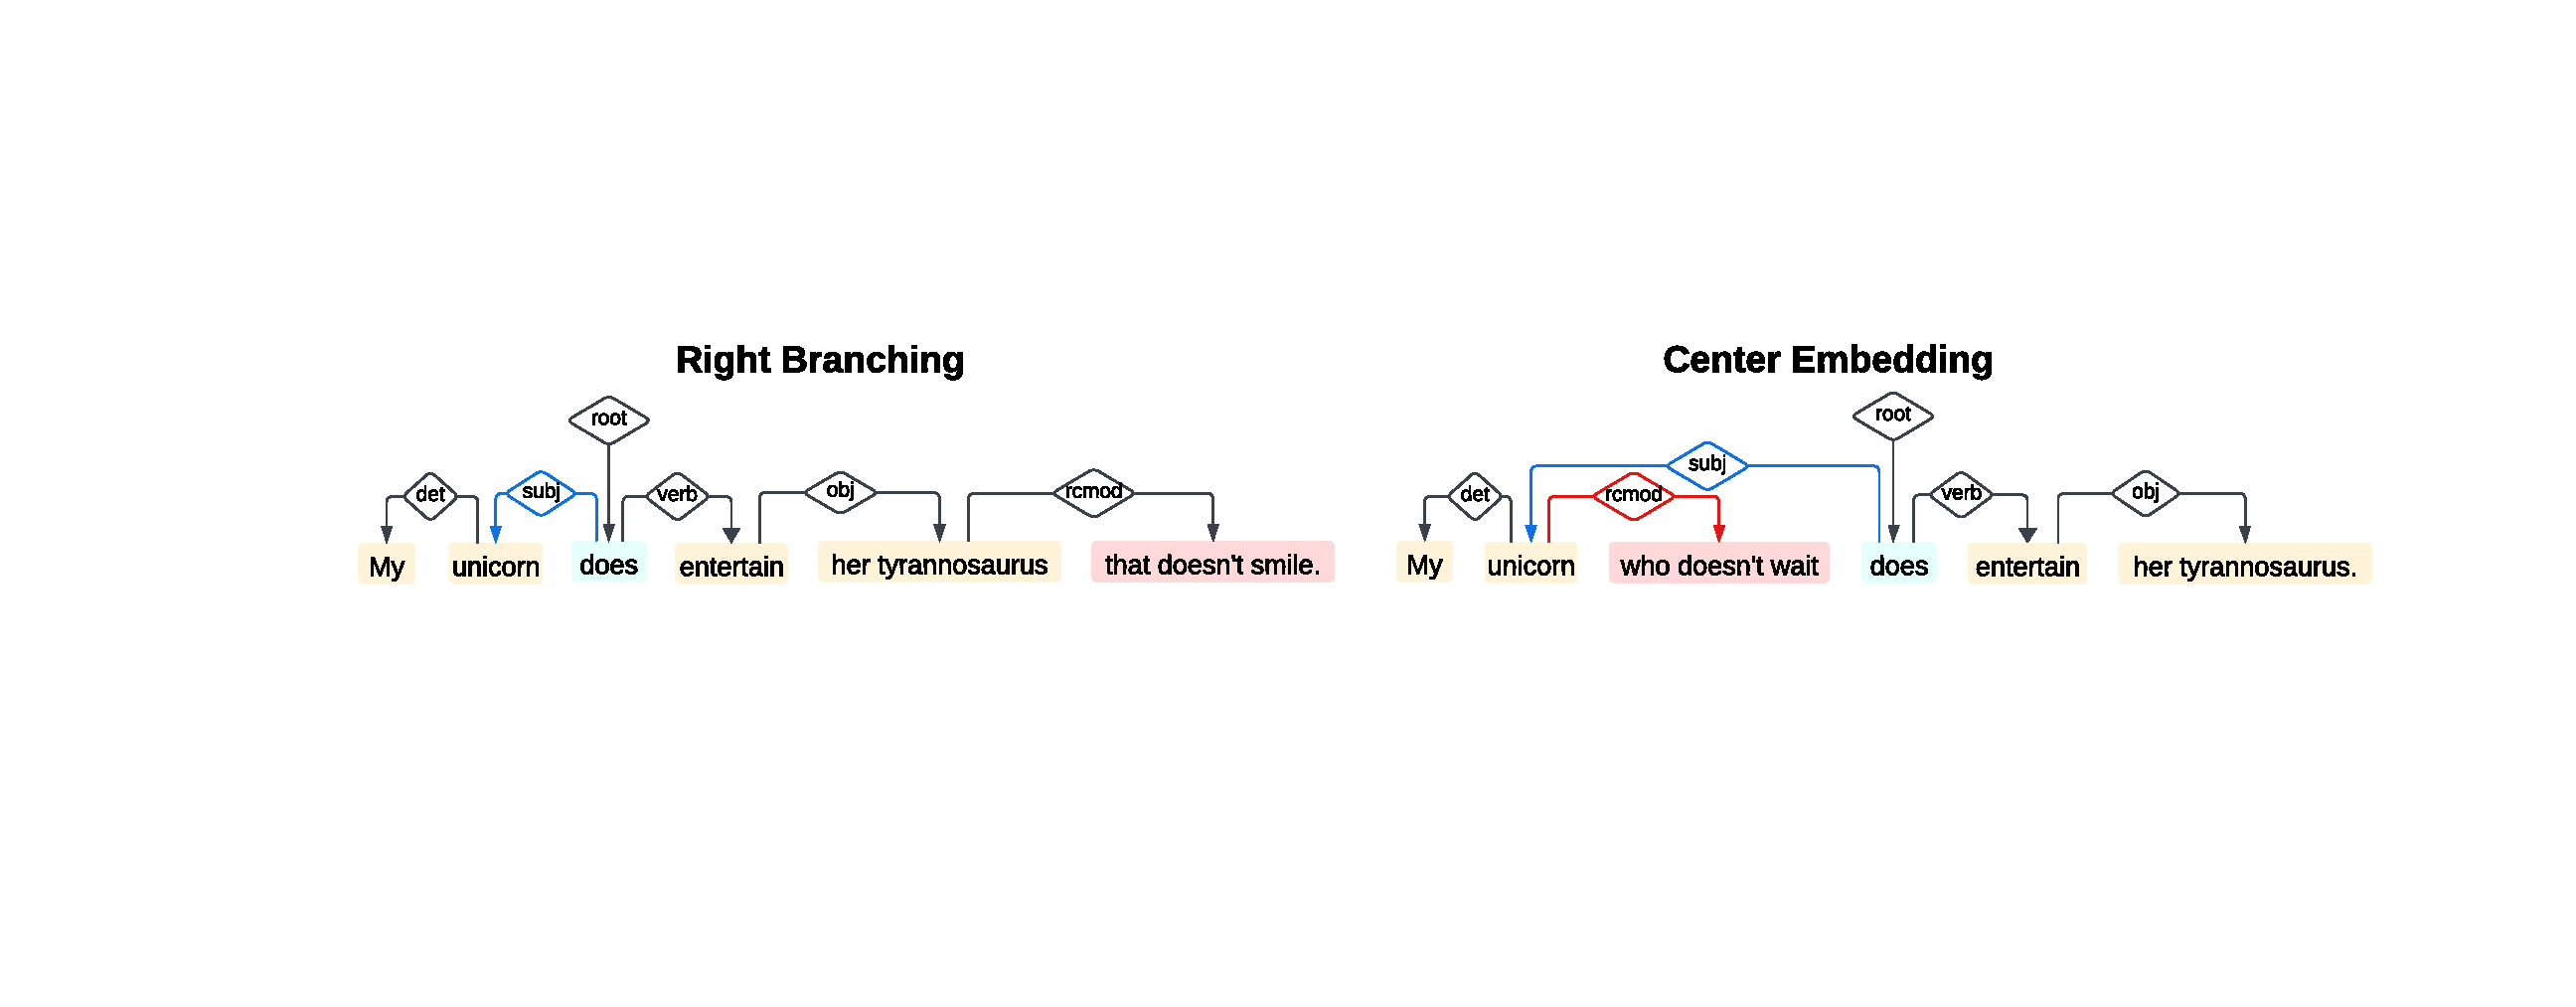
\includegraphics[width=1.0\textwidth]{figures/sentence_demo.pdf}
    \caption{\textbf{Sentence Examples.}   \textit{Left:} Right-branching sentence example. The linear progression of the main constituent is not interrupted by the relative clause. 
    \textit{Right:} Center-embedded sentence example. When the relative clause modifies the subject, it interrupts the linear progression of the main constituent. 
    }
    \label{fig:sentence_demo}
\end{figure}

\subsection{Center Embedding}
\label{sec:center_embed}
Center embedding occurs when a clause is placed recursively within another clause of the same type. Figure \ref{fig:sentence_demo} (\textit{left}) illustrates two examples of center-embedded sentences, where the embedded clause complicates syntactic parsing by placing an additional subject noun in between a verb and its own subject. Whereas center embeddings exhibit a recursive structure, sentences without center embeddings are exclusively right-branching. Right-branching structures may also include modifying clauses, but these clauses can only be appended at the end of the main clause, maintaining its linear flow (see Figure \ref{fig:sentence_demo}, \textit{right}). Linguists have long argued that center embeddings play a crucial role in grammar acquisition \citep{wexler1980formal} and give rise to tree-like syntactic structures \citep{Chomsky2015-bg}. 


We find that center embeddings, which are crucial for human language acquisition, also lead an LM to acquire hierarchical grammar rules. To correctly predict the next token, LMs must track syntactic connections between words in the context. In right-branching sentences, LMs can rely on linear proximity to identify these connections; as shown in Figure \ref{fig:sentence_demo}, a simple bigram model suffices to capture the subject-verb relationship for such sentences. In contrast, center embeddings introduce relative clauses of various lengths, making linear n-gram models inefficient for capturing subject-verb relationships. The recursive nature of the center embedding requires the model to track multiple subject-verb relationships: one for the main clause and a separate one for the embedded relative clause. In these cases, a tree structure is more efficient to model subject-verb relationships. 


\subsection{Question Formation Results}
\label{sec:qf_result}
As specified in Section \ref{sec:qf_task}, the training data for QF is ambiguous between the linear rule (i.e., moving the first auxiliary) and the hierarchical rule (i.e., moving the main auxiliary). Center-embedded sentences do not meet this ambiguity requirement and, therefore, cannot appear in question formation training samples. To ensure the model is exposed to diverse sentence types, \citet{McCoy2018-uv} introduced a secondary task to the QF training dataset: declaration copying. Like question formation, the declaration-copying example starts with a declarative sentence, but instead of transforming it, the model simply repeats it. Since the ambiguity requirement only applies to the primary question formation task, declaration-copying examples can include center embeddings. Concrete examples of both tasks can be found in Appendix \ref{appdx:data_sample}.


We train models on three modifications of the original training data, varying the composition of the declaration-copying subset. 
In \textit{Quest Only}, we remove all declaration-copying examples.
In \textit{Center embed}, we only keep center-embedded examples. In \textit{Right branch}, we only keep right-branching examples. 
Every modified training sets retains all examples of the primary task, question formation.
Every model trained, regardless of its training set composition, reaches 100\% in-distribution validation accuracy; however, the OOD generalization performance, shown in Figure \ref{fig:grokking_selection} (\textit{left}), differs significantly across the modified training sets. 

Our results confirm that declaration copying examples, specifically center embeddings, are essential for inducing hierarchical generalization.
Models trained without any declaration-copying examples fail to achieve an OOD accuracy above 75\%; so do models trained \textit{only} on right-branching  declaration-copying examples. When trained instead \textit{only} on center-embedded declaration-copying examples, models exhibit a strong preference for the hierarchical rule. This evidence suggests that center-embedded sentences direct a model towards the hierarchical rule. 

\begin{figure}[t!]
    \centering
    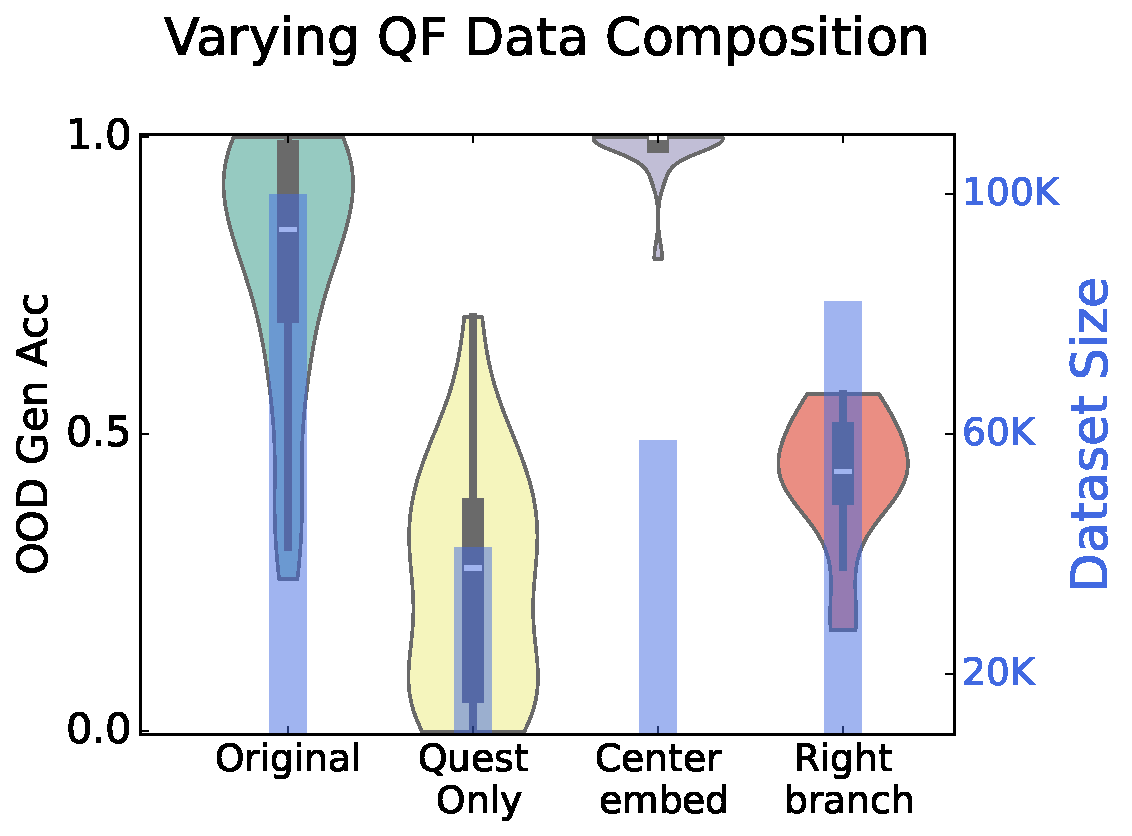
\includegraphics[width=0.41\linewidth]{figures/no_curriculum_main.pdf}
    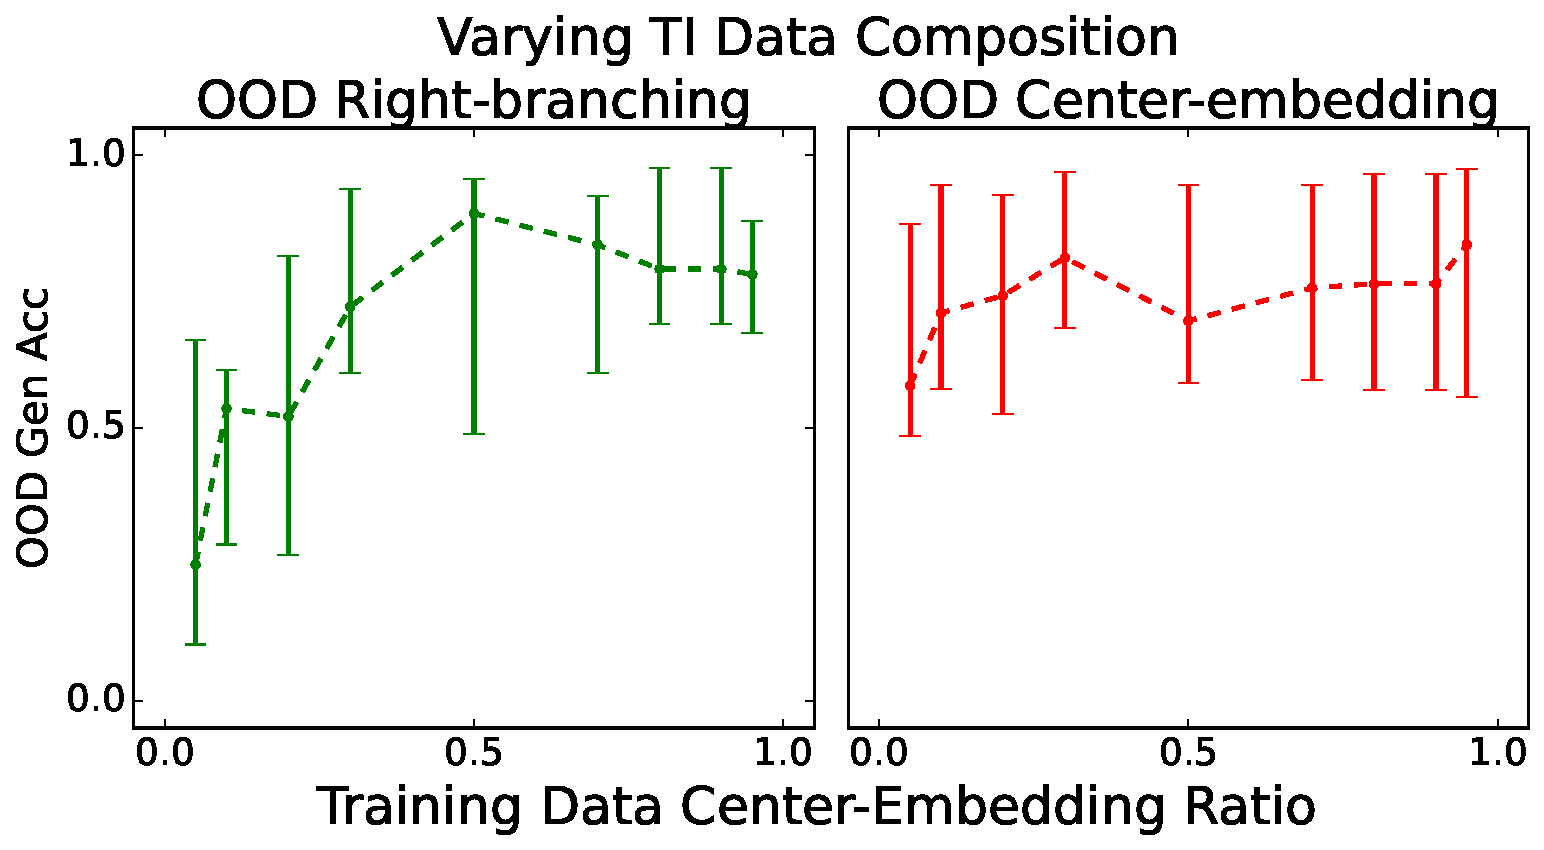
\includegraphics[width=0.55\linewidth]{figures/ti_simplicity_contamination.pdf}
    \caption{
    \textbf{Components of training data drive different generalization behaviors.} 
    \textit{Left:} Center-embedded sentences, which in the QF training data only appear in declaration copying examples, induce hierarchical generalization.
    \textit{Right:} Models are trained on different TI training data mixes and evaluated on two OOD sets: unambiguous right-branching sentences (\textit{green}) and unambiguous center-embedded sentences (\textit{red}). For center-embedded sentences, the hierarchical rule is preferred regardless of data mixes. For right-branching sentences, the model's preference for the hierarchical rule is exclusively driven by having a large mix of center-embedded sentences in the TI training data.}
    \label{fig:grokking_selection}
\end{figure}



\subsection{Tense Inflection Results}
\label{sec:ti_result}

In the TI training data, both right-branching and center-embedded sentences are made ambiguous by ensuring the distractor noun (i.e., a noun that appears between the main subject and the main verb) shares the same plurality as the main subject. For right-branching sentences, the distractor noun occurs in a prepositional phrase. For center-embedded sentences, the distractor noun occurs in a relative clause; either the subject or the object of the modifying clause can act as the distractor noun. We list examples below: 

\begin{enumerate}[itemsep=2pt,labelindent=10pt,topsep=0pt,parsep=0pt,partopsep=1pt, align=left, leftmargin=*]
    \item \textbf{Right Branching}: The noun in the prepositional phrase (e.g., `` \textit{to the cabinet}") acts as the distractor in the TI task.
    
    Example A (ID): \textit{The keys to the \textbf{cabinets} are on the table.}

    Example B (OOD): \textit{The keys to the \textbf{cabinet} are on the table.}
    
    \item \textbf{Center Embedding}: Either the subject or the object inside the relative clause acts as the distractor in the TI task.

    Example C (ID): \textit{The keys that unlock the \textbf{cabinets} are on the table.}

    Example D (OOD): \textit{The keys that unlock the \textbf{cabinet} are on the table.}
    
    
\end{enumerate}
We create variations of the TI training data by adjusting the ratio of right-branching to center-embedded samples while keeping the total training size constant.\footnote{The original training dataset contains a secondary past-tense copying task, to parallel the declaration-copying secondary task in QF. We show in Appendix \ref{appdx:ti_secondary} that the secondary task is not necessary, and we do not include it in our modified training sets.} A model's generalization behavior is tested on two OOD sets: one containing unambiguous right-branching sentences (e.g., Example B) and the other containing unambiguous center-embedded sentences (e.g., Example D). 

Generalization accuracies are shown in Figure \ref{fig:grokking_selection} (\textit{right}). When the training data is dominated by ambiguous right-branching sentences, the model fails to learn the hierarchical rule, as indicated by low OOD accuracy. However, when trained on a greater proportion of center-embedded sentences, the model systematically applies the hierarchical rule to both right-branching and center-embedded OOD sentences. As shown in Figure \ref{fig:grokking_selection} (\textit{right}), regardless of its training data mix, the model  generalizes hierarchically to OOD \textit{center embeddings}. In contrast, the model only generalizes hierarchically to \textit{right-branching sentences} after being exposed to a sufficient quantity of center-embedded sentences during training. In other words, the model eventually learns to treat non-recursive sequences as hierarchical through exposure to recursive center embeddings. These observations suggest that center embeddings drive the model's overall preference for tree structures. For further analysis of which center embedding structures induce this bias most efficiently, see Appendix \ref{appdx:obj_sbj_ctr_breakdown}.

% %%%%%%%%%%%%%%%%Previous version to preserve comments %%%%%%%%%%%%%%%%%%%%%%%%%%%%%%%%%%%%%%%%
% \iffalse
% \subsection{Tense Inflection} 
% \label{sec:ti_result}
% We now analyze hierarchical generalization in the tense inflection task, demonstrating the generality of our findings across grammatical rules. 
% The tense inflection setting from \citet{Linzen2016-vx} uses the same generation process as the question formation task, changing only the task itself.  
% This generation process leads to three types of sentences:

% \begin{enumerate}[itemsep=2pt,labelindent=10pt,topsep=0pt,parsep=0pt,partopsep=1pt, align=left, leftmargin=*]
%     \item The main verb immediately follows the subject noun.

%     Example: \textit{The keys are on the table.}
%     \item The main verb and the subject noun are separated by a prepositional phrase (e.g., `` \textit{to the cabinet}"). In all sentence examples, the prepositional phrase consistently follows the same syntactical structure and length (i.e., ``preposition $+$ determiner $+$ noun"). 

%     Example: \textit{The keys to the cabinet are on the table.}
%     \item The main verb and subject noun are separated by a relative clause, which can vary in syntactic composition and length.

%     Example: \textit{The keys that I used to unlock the cabinet are on the table.}
% \end{enumerate}


% By definition, both the first and second sentence types are right branching. In the second type, although a prepositional phrase is inserted within the main clause, it differs syntactically from a relative clause modifier. Unlike relative clause modifiers, prepositional phrases lack syntactic diversity, whereas relative clauses can exhibit the same of diversity as an entire sentence. In QF and TI data generated by CFG rules, a 4-gram model suffices to capture the subject-verb agreement. In contrast, relative clause modifiers (i.e., the third type) vary in both length and syntactic structure. All three sentence types are present in the original training data. Since sentences of the first type lack a distractor noun, they cannot be used to probe the model’s generalization, so the generalization set includes only the second and third types. As specified in Section \ref{sec:ti_task}, the TI training data only requires that the subject and distractor have the same plurality. Thus, center-embedded sentences can be included in the TI training data without violating the ambiguity requirement, and a secondary task is not necessary for TI.\footnote{In Appendix \ref{appdx:tense_tv}, we show that we can again leverage a secondary task such that a model trained on center-embedded tense inflection examples can generalize to right-branching sentences without having seen any examples of tense inflection on the sentence type, but not vice versa. }


% Our goal is to verify that center embeddings also drive OOD generalization in tense inflection. We create variations of the TI training data by adjusting the ratio of right-branching to center-embedded sentences, keeping the total training size constant. In Figure \ref{fig:ti_selection}, we report the model's OOD behavior across two data partitions. Figure \ref{fig:ti_selection} (\textit{left}) shows the model's generalization accuracy on unambiguous right-branching sentences when trained on different data mixes. When training data is dominated by ambiguous right-branching sentences, the model fails to learn the hierarchical rule, as indicated by low OOD generalization accuracy. However, as we increase the proportion of center-embedded sentences, these sentences---despite being ambiguous---bias the model towards the hierarchical rule, reflected by improved generalization accuracy.

% Figure \ref{fig:ti_selection} (\textit{right}) shows that the model consistently prefers the hierarchical rule for center-embedded sentences, regardless of data composition. These results indicate that the model’s preference for the hierarchical rule is primarily driven by center-embedded sentences. Moreover, with a high proportion of center-embedded sentences in the training data, this hierarchical rule preference extends to right-branching sentences as well.


% \fi

%%%%%

We conducted ablation studies on some of the designs mentioned in Section~\ref{sec:model} to verify their effectiveness.


\subsection{Position Embedding}
First, we compared 3D RoPE with sinusoidal absolute position encoding. As shown in Figure~\ref{fig:d}, the loss curve using 3D RoPE converges significantly faster than that with sinusoidal encoding.
Then we compared the use of 3D RoPE alone with the combination of 3D RoPE and learnable absolute position embedding. As shown in Figure~\ref{fig:c}, the loss curves of both methods converge almost identically. For simplicity, we chose to use 3D RoPE alone.

\subsection{Expert Adaptive Layernorm}
We experimented with different ways of incorporating experts: expert LayerNorm and MLP, and expert Layernorm only. Our experiments found that adding expert MLP does not effectively accelerate the model's convergence (Figure~\ref{fig:b}). To reduce the model parameters, we only chose to use expert adaptive Layernorm.

\section{Empirical Evaluation}
We trained a series of models of various sizes. For all subsequent evaluations, we will use the largest model (referred to as CogVideoX).
In this section, we present the experimental validation of CogVideoX through two primary methods: automated metric evaluation and human assessment, providing a thorough analysis of the performance and quality of the generated videos. 
We trained a series of models with different parameter sizes. The following evaluation defaults to using our largest model.

\subsection{Results of Automated Metric Evaluation} 

\paragraph{Baselines.} We chose several top-performing text-to-video models as our baselines for comparison, including T2V-Turbo~\citep{li2024t2v}, AnimateDiff~\citep{guo2023animatediff}, VideoCrafter2~\citep{chen2024videocrafter2}, OpenSora~\citep{opensora}, Show-1~\citep{zhang2023show}, Gen-2~\citep{gen2}, Pika~\citep{pika} and LaVie-2~\citep{wang2023lavie}.


% \begin{figure}[h]
% \begin{center}
% \includegraphics[width=0.9\linewidth]{images/bench_eval.png}
% \end{center}
% \caption{The radar chart comparing the performance of different models.}
% \label{fig:radar}
% \end{figure}

\hide{
%\begin{wrapfigure}{r}{0.5\textwidth}
\begin{figure}
\centering
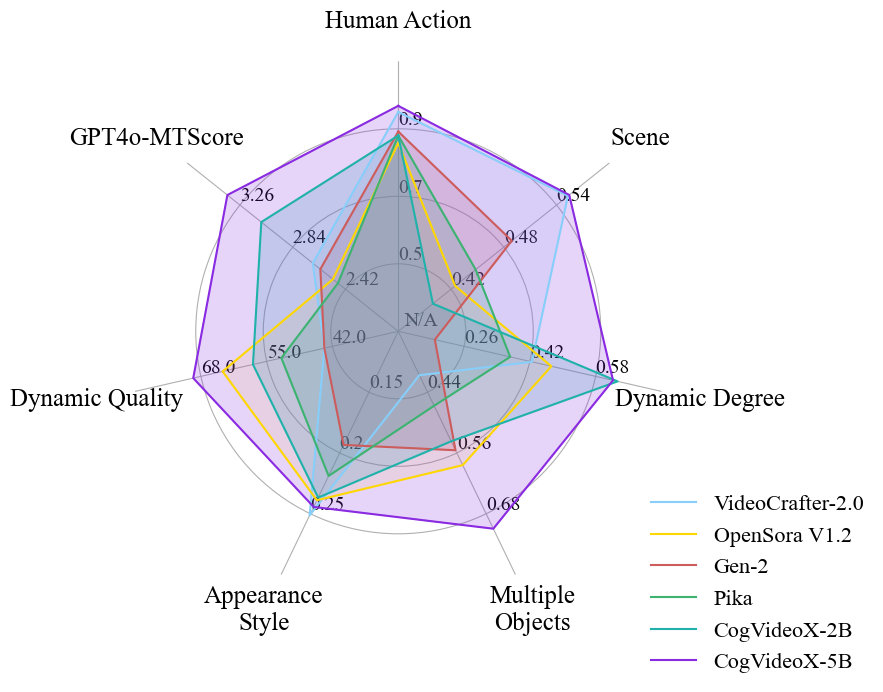
\includegraphics[width=0.7\linewidth]{images/bench_eval9.png}
\caption{The radar chart comparing the performance of different models. CogVideoX represents the largest one. It is clear that CogVideoX outperforms its competitors in the vast majority of metrics, and it is very close to the leading models in the remaining indicator.
}
\label{fig:radar}
% \vspace{-10mm}
%\end{wrapfigure}

\end{figure}

}%end ofhide
\paragraph{Evaluation Metrics.} To evaluate the text-to-video generation, we employed several metrics from VBench~\citep{huang2023vbench}: \emph{Human Action}, \emph{Scene}, \emph{Dynamic Degree}, \emph{Multiple Objects}, and \emph{Appearance Style}. VBench is a suite of tools designed to automatically assess the quality of generated videos. We have selected certain metrics from VBench, excluding others that do not align with our evaluation needs. For example, the color metric, intended to measure the presence of objects corresponding to specific colors across frames in the generated video, assesses the model's quality by calculating the probability. However, this metric may mislead video generation models that exhibit greater variation, thus we chose not to include it in our evaluation. For longer-generated videos, some models might produce videos with minimal changes between frames to obtain higher scores, but these videos lack rich content. Therefore, a metric for evaluating the dynamism of the video becomes more important. To address this, we employed two video evaluation tools, We also employed the \emph{Dynamic Quality} from Devil~\citep{liao2024evaluationtexttovideogenerationmodels} and \emph{GPT4o-MTScore} from ChronoMagic~\citep{yuan2024chronomagic}, which focus more on the dynamic characteristics of videos. \emph{Dynamic Quality} is defined by the integration of various quality metrics with dynamic scores. This approach mitigates biases arising from negative correlations between video dynamics and video quality, leading to a more thorough assessment of video quality. ChronoMagic, for instance, introduces the \emph{GPT4o-MTScore}, a metric designed to measure the metamorphic amplitude of time-lapse videos, such as those depicting physical, biological, and meteorological changes. This metric is obtained by extracting frames from the generated videos at regular intervals and using GPT-4o~\citep{gpt4o} to score the degree of change, providing a fine-grained assessment of video dynamism. This method ensures a more accurate evaluation of the content's variability over time, countering the potential bias of static frame sequences in scoring.



\paragraph{Results.} Table~\ref{table:results} provides a detailed comparison of the performance of our CogVideoX model with other models. Our model achieved the best performance in 5 out of the 7 metrics and showed competitive results in the remaining 2 metrics. These results demonstrate that our model not only excels in video generation quality but also outperforms previous models in handling various complex dynamic scenes. Additionally, Figure~\ref{fig:radar} presents a radar chart comparing the performance of different models.


\begin{figure}[ht]
\begin{center}
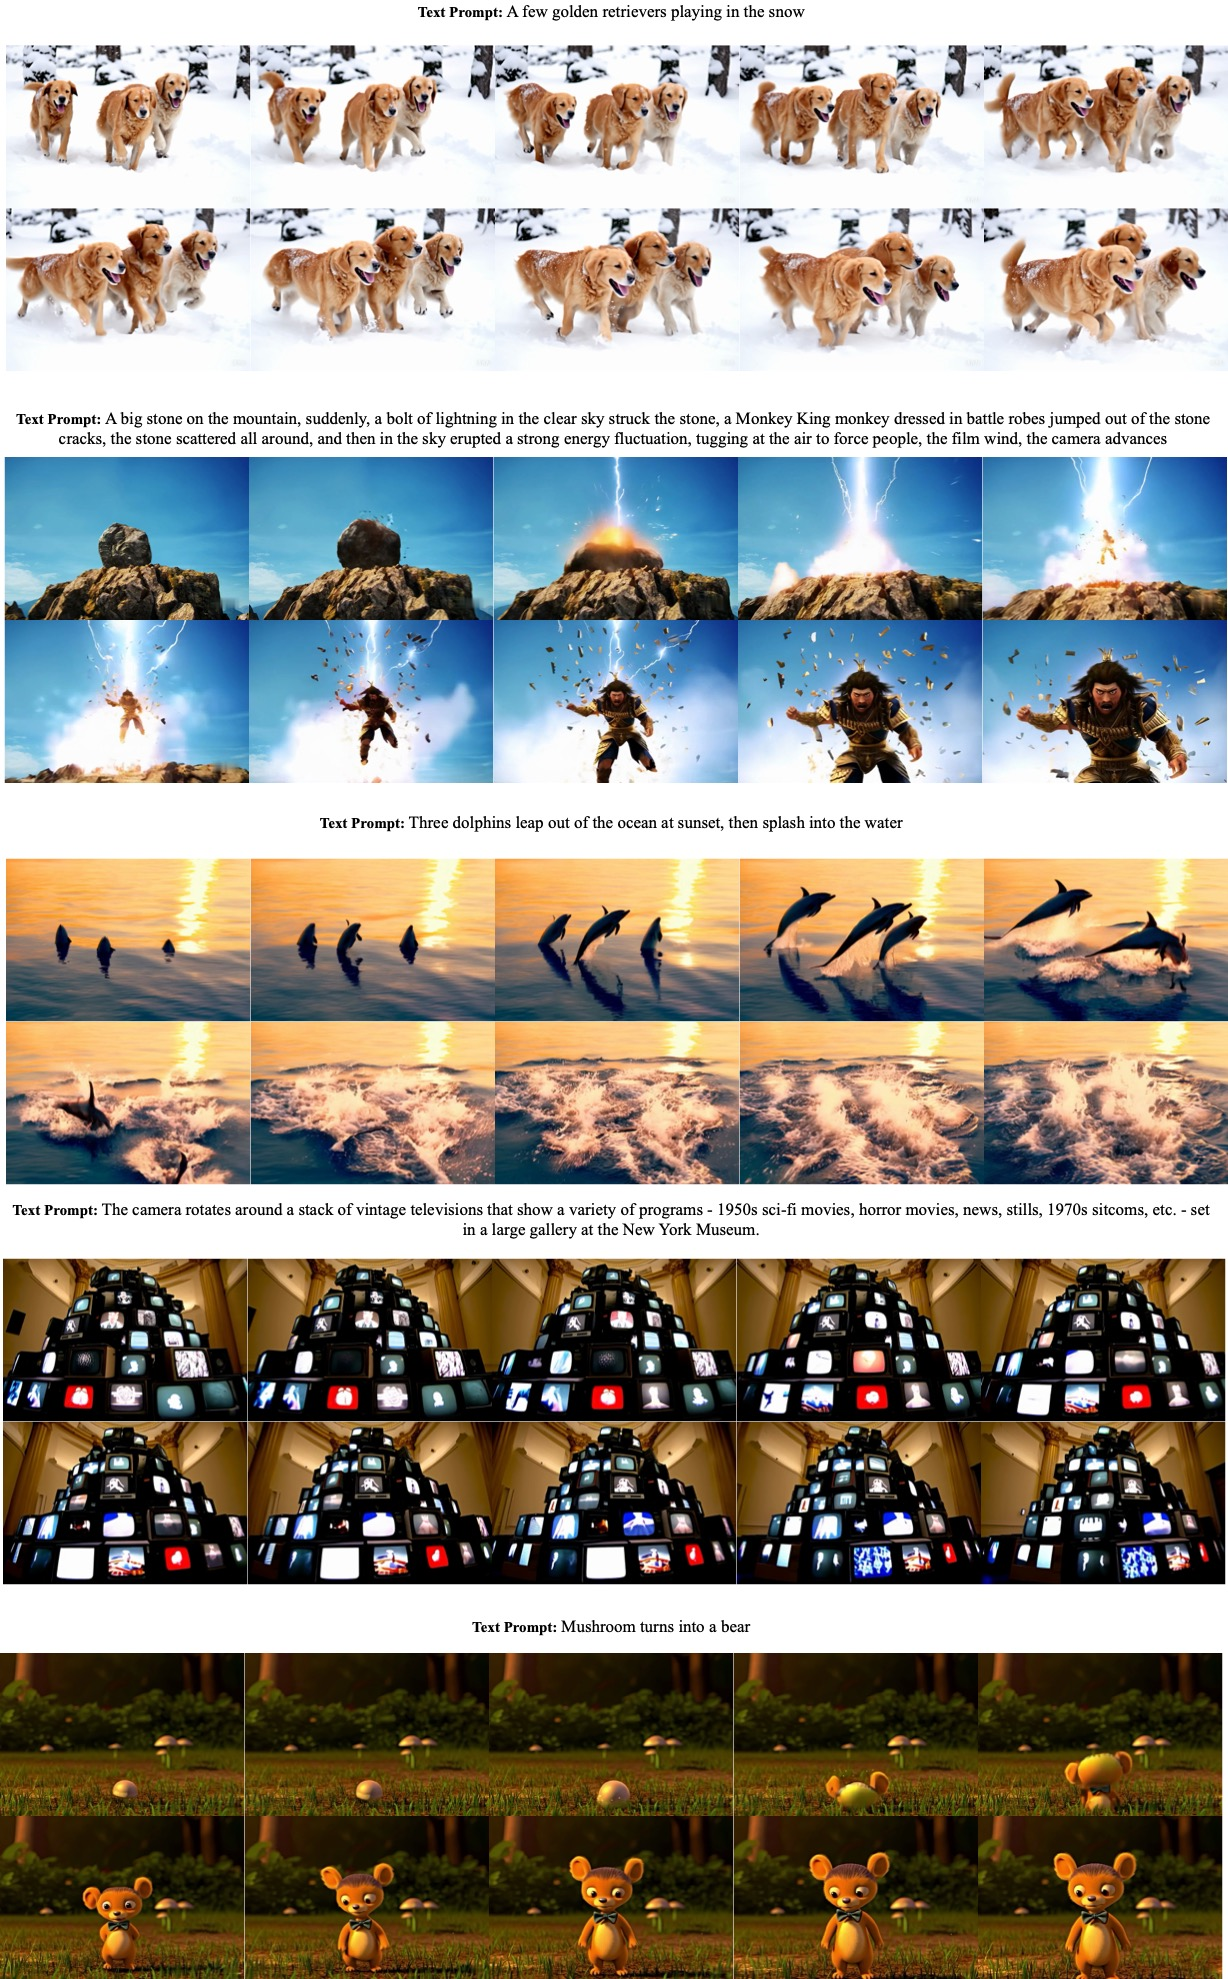
\includegraphics[width=\linewidth]{images/t2v/goodcase1.jpg}
\end{center}
\caption{Text to video showcases. The displayed prompt will be upsampled before being fed into the model. The generated videos contain large motion and can produce various video styles.}
\label{fig:t2vgood1}
\end{figure}

\begin{figure}[ht]
\begin{center}
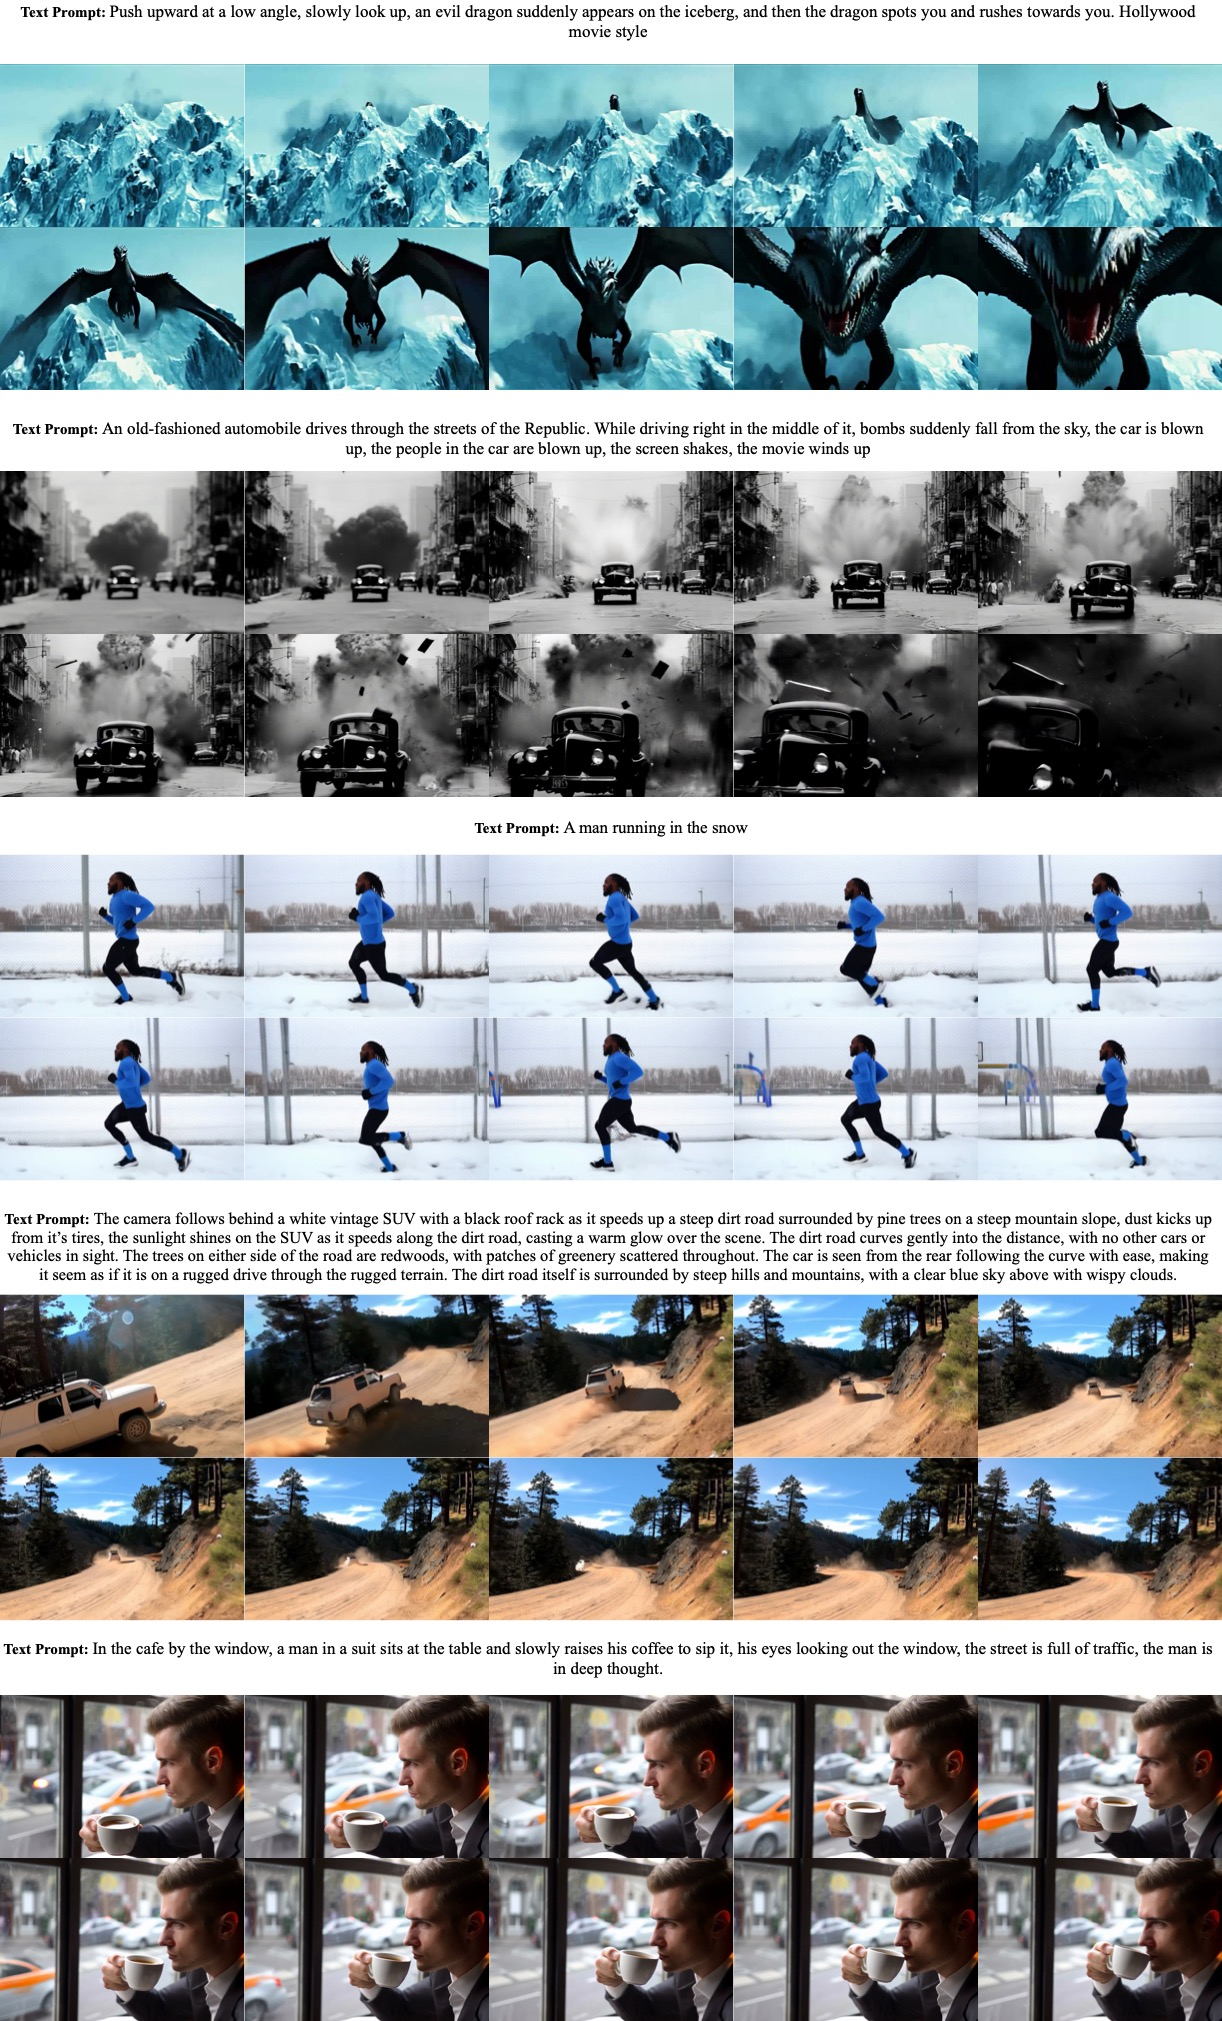
\includegraphics[width=0.98\linewidth]{images/t2v/goodcase2.jpg}
\end{center}
\caption{Text to video showcases.}
\label{fig:t2vgood2}
\end{figure}


% Please add the following required packages to your document preamble:
% \usepackage[table,xcdraw]{xcolor}
% Beamer presentation requires \usepackage{colortbl} instead of \usepackage[table,xcdraw]{xcolor}
% \usepackage[normalem]{ulem}
% \useunder{\uline}{\ul}{}




% \begin{table}[]

% \centering
% \setlength\tabcolsep{3pt}

% \label{sample-table}
% \small
% \vspace{-10pt}
% \caption{\textbf{Automatic Evaluation Results per Dimension.}The table presents a comparative analysis of various video models across different dimensions. It is evident from the table that, in terms of both human motion and background effects as well as the accuracy and distinctiveness of objects, CogVideoX has achieved the current SOTA level. Furthermore, CogVideoX has garnered a commendable score in the expression of dynamic qualities, a capability that serves as a more precise indicator of the intrinsic properties of video media, distinct from the static nature of photographic images.}

% \vspace{6pt}

% \begin{tabular}{cccccccc}
% \toprule
% \multirow{2}{*}{\textbf{Models} }  & \textbf{human}  & \textbf{object} &\multirow{2}{*}{\textbf{scene}}&\textbf{dynamic} &\textbf{multiple} &\textbf{spatial} &\textbf{appearance} \\
%     & \textbf{action}& \textbf{class}& & \textbf{degree} &\textbf{objects}& \textbf{relationship}&\textbf{style}  
% \\
% \midrule
% CogVideoX & 96.80\% &93.70\% & 55.44\% & 62.22\% & 70.95\% & 61.29\% & 24.44\% \\
% {LaVie-2} & 96.40\% & 97.52\%  & 49.59\% & 31.11\% & 64.88\%  & 38.68\% & 25.09\%  \\
% {T2V-Turbo}  & 95.20\%  & 93.96\%& 55.58\% & 49.17\% & 54.65\%    & 38.67\%  & 24.42\%   \\
% {Gen-2}  & 89.20\%& 90.92\%  & 48.91\%  & 18.89\% & 55.47\%    & 66.91\%   & 19.34\%  \\
% {VideoCrafter-2.0\citep{chen2024videocrafter2}} & 95.00\% & 92.55\% & 55.29\%               & 42.50\% & 40.66\% & 35.86\% & 25.13\%  \\
% {Pika Beta} & 88.00\% & 87.45\%  & 44.80\% & 37.22\% & 46.69\% & 65.65\% & 21.89\%   \\
% AnimateDiff-V2 & 92.60\% & 90.90\%  & 50.19\% & 40.83\%        & 36.88\% & 34.60\%  & 22.42\%\\
% {OpenSora V1.2}   & 85.80\% & 83.37\%& 42.47\%   & 47.22\%    & 58.41\% & 67.51\%  & 23.89\%  \\
% {Show-1} & 95.60\%  & 93.07\%  & 47.03\% & 44.44\% & 45.47\% & 53.50\%  & 23.06\%  \\
% {HiGen}  & 86.20\%  & 86.06\%  & 44.88\% & 99.17\% & 22.39\%  & 22.43\% & 24.54\% \\  
% \bottomrule
% \end{tabular}
% \end{table}



% \iffalse



% \begin{table}[ht!]
% \centering
% \caption{Evaluation results.}
% \setlength\tabcolsep{3pt}
% \label{sample-table}
% \begin{center}
% \small
% \resizebox{0.9\linewidth}{!}{
% \begin{tabular}{ccccccccc}

% \multirow{2}{*}{\textbf{Models} }  & \textbf{subject}  & \textbf{background} &\textbf{temporal} &\textbf{motion} &\textbf{dynamic} &\textbf{aesthetic} &\textbf{imaging} &\textbf{object} \\
%     & \textbf{consistency}& \textbf{consistency}& \textbf{flickering}& \textbf{smoothness} &\textbf{degree}& \textbf{quality}&\textbf{quality} & \textbf{class}
% \\ \hline 
%         CogVideoX & 94.66\% & 95.92\% & 97.47\% & 98.10\% & 62.22\% & 55.14\% & 63.62\% & 93.70\%  \\
%         LaVie-2 & 97.90\% & 98.45\% & 98.76\% & 98.42\% & 31.11\% & 67.62\% & 70.39\% & 97.52\%  \\ 
%         T2V-Turbo (VC2) & 96.28\% & 97.02\% & 97.48\% & 97.34\% & 49.17\% & 63.04\% & 72.49\% & 93.96\%  \\ 
%         Gen-2 (2023-06) & 97.61\% & 97.61\% & 99.56\% & 99.58\% & 18.89\% & 66.96\% & 67.42\% & 90.92\%  \\ 
%         VideoCrafter-2.0\citep{chen2024videocrafter2} & 96.85\% & 98.22\% & 98.41\% & 97.73\% & 42.50\% & 63.13\% & 67.22\% & 92.55\%  \\ 
%         Pika Beta (2023-06) & 96.76\% & 98.95\% & 99.77\% & 99.51\% & 37.22\% & 63.15\% & 62.33\% & 87.45\%  \\ 
%         AnimateDiff-V2 & 95.30\% & 97.68\% & 98.75\% & 97.76\% & 40.83\% & 67.16\% & 70.10\% & 90.90\%  \\ 
%         OpenSora V1.2 & 94.45\% & 97.90\% & 99.47\% & 98.20\% & 47.22\% & 56.18\% & 60.94\% & 83.37\%  \\ 
%         Show-1 & 95.53\% & 98.02\% & 99.12\% & 98.24\% & 44.44\% & 57.35\% & 58.66\% & 93.07\%  \\ 
%         HiGen & 90.07\% & 93.99\% & 93.24\% & 96.69\% & 99.17\% & 57.30\% & 63.92\% & 86.06\% \\ 
% \hline \\

% \multirow{2}{*}{\textbf{Models} }  & \textbf{multiple}  & \textbf{human} &\multirow{2}{*}{\textbf{color}} &\textbf{spatial} &\multirow{2}{*}{\textbf{scene}} &\textbf{appearance} &\textbf{temporal} &\textbf{overall} \\
%     & \textbf{objects}& \textbf{action}& & \textbf{relation} & & \textbf{style}&\textbf{style} & \textbf{consistency}
% \\ \hline 
%         CogVideoX & 70.95\% & 96.80\% & 79.75\% & 61.29\% & 55.44\% & 24.44\% & 23.69\% & 26.73\%  \\ 
%         LaVie-2 & 64.88\% & 96.40\% & 91.65\% & 38.68\% & 49.59\% & 25.09\% & 25.24\% & 27.39\%  \\ 
%         T2V-Turbo (VC2) & 54.65\% & 95.20\% & 89.90\% & 38.67\% & 55.58\% & 24.42\% & 25.51\% & 28.16\%  \\
%         Gen-2 (2023-06) & 55.47\% & 89.20\% & 89.49\% & 66.91\% & 48.91\% & 19.34\% & 24.12\% & 26.17\%  \\ 
%         VideoCrafter-2.0 & 40.66\% & 95.00\% & 92.92\% & 35.86\% & 55.29\% & 25.13\% & 25.84\% & 28.23\%  \\
%         Pika Beta (2023-06) & 46.69\% & 88.00\% & 85.31\% & 65.65\% & 44.80\% & 21.89\% & 24.44\% & 25.47\%  \\ 
%         AnimateDiff-V2 & 36.88\% & 92.60\% & 87.47\% & 34.60\% & 50.19\% & 22.42\% & 26.03\% & 27.04\%  \\ 
%         OpenSora V1.2 & 58.41\% & 85.80\% & 87.49\% & 67.51\% & 42.47\% & 23.89\% & 24.55\% & 27.07\%  \\ 
%         Show-1 & 45.47\% & 95.60\% & 86.35\% & 53.50\% & 47.03\% & 23.06\% & 25.28\% & 27.46\%  \\ 
%         HiGen & 22.39\% & 86.20\% & 86.22\% & 22.43\% & 44.88\% & 24.54\% & 25.14\% & 27.14\% \\ \hline

% \hline \\
% \end{tabular}

% }
% \end{center}
% \end{table}

% \fi






% \begin{table}[!ht]
% \centering

% \label{sample-table}
% \small
% \vspace{-10pt}
% \caption{\textbf{Automatic Evaluation Results per Dimension.}}

% \vspace{6pt}

% \resizebox{0.8\linewidth}{!}{
%     \begin{tabular}{cccc}
%         \textbf{Models} & \textbf{\Centerstack{Dynamics Range}} & \textbf{\Centerstack{Dynamics Controllability}} & \textbf{\Centerstack{Dynamics-based Quality}} \\ \hline
%         CogVideoX       & 55.7 & 71.8 & \textbf{69.5} \\ 
%         Gen-2           & 30.8 & \textbf{82.5} & 43.6 \\ 
%         Pika            & 43.2 & 72.0 & 52.1 \\ 
%         VideoCrafter2   & 34.1 & 57.0 & 43.6 \\ 
%         OpenSora        & \textbf{61.2} & 62.4 & 63.7 \\ 
%         Show-1          & 45.1 & 73.9 & 57.7 \\ 
%     \end{tabular}
% }
% \end{table}


% \begin{figure}[h]
% \begin{center}
% \includegraphics[width=0.9\linewidth]{images/bench_eval.png}
% \end{center}
% \caption{The radar chart comparing the performance of different models.}
% \label{fig:radar}
% \end{figure}

\hide{
%\begin{wrapfigure}{r}{0.5\textwidth}
\begin{figure}
\centering
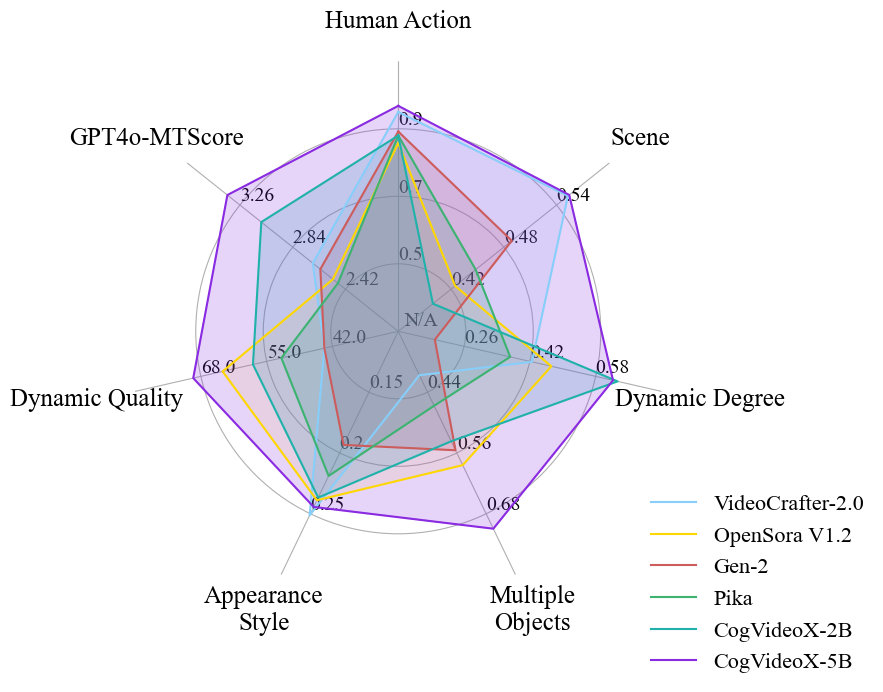
\includegraphics[width=0.7\linewidth]{images/bench_eval9.png}
\caption{The radar chart comparing the performance of different models. CogVideoX represents the largest one. It is clear that CogVideoX outperforms its competitors in the vast majority of metrics, and it is very close to the leading models in the remaining indicator.
}
\label{fig:radar}
% \vspace{-10mm}
%\end{wrapfigure}

\end{figure}

}%end ofhide


\subsection{Human Evaluation}
In addition to automated scoring mechanisms, a comparative analysis between the Kling~\citep{kling} and CogVideoX was conducted using a manual scoring system. One hundred meticulously crafted prompts were used, characterized by their broad distribution, clear articulation, and well-defined conceptual scope. We randomize videos for blind evalution. A panel of evaluators assigned scores for each detail on a scale from zero to one, with the overall total score rated on a scale from zero to five, where higher scores reflect better video quality. Reasons for any score deductions were also carefully documented. The results shown in Table~\ref{table:human_eva} indicate that our model outperforms Kling in all aspects. More details are shown in \ref{sec:human_evalution}.

\begin{table}[!ht]
\centering
\label{sample-table}
\small
\vspace{-5pt}
\caption{Human evaluation between CogVideoX and Kling.}
\label{table:human_eva}
\resizebox{0.75\linewidth}{!}{
    \begin{tabular}{cccccc}
    \toprule
        Model & \Centerstack{Sensory\\Quality} & \Centerstack{Instruction\\Following}&\Centerstack{Physics\\Simulation} & \Centerstack{Cover\\Quality} & 
        \Centerstack{Total\\Score} \\ 
        \midrule
        Kling & 0.638 & 0.367 & 0.561 & 0.668 & 2.17 \\
        \midrule
         {\bf CogVideoX-5B} & {\bf 0.722} & {\bf 0.495} & {\bf 0.667} & {\bf 0.712} & {\bf 2.74}  \\
        \bottomrule
    \end{tabular}
}
\vspace{-3mm}
\end{table}



% \begin{table}[!ht]
% \centering

% \label{sample-table}
% \small
% \vspace{-10pt}
% \caption{\textbf{Automatic Evaluation Results per Dimension.}}

% \vspace{6pt}

% \resizebox{0.8\linewidth}{!}{
%     \begin{tabular}{cccc}
%         \textbf{Models} & \textbf{\Centerstack{Dynamics Range}} & \textbf{\Centerstack{Dynamics Controllability}} & \textbf{\Centerstack{Dynamics-based Quality}} \\ \hline
%         CogVideoX       & 55.7 & 71.8 & \textbf{69.5} \\ 
%         Gen-2           & 30.8 & \textbf{82.5} & 43.6 \\ 
%         Pika            & 43.2 & 72.0 & 52.1 \\ 
%         VideoCrafter2   & 34.1 & 57.0 & 43.6 \\ 
%         OpenSora        & \textbf{61.2} & 62.4 & 63.7 \\ 
%         Show-1          & 45.1 & 73.9 & 57.7 \\ 
%     \end{tabular}
% }
% \end{table}





Hyperbolic embeddings embed hierarchical information with high
fidelity and few dimensions. We explored the limits of this approach
by describing scalable, high quality algorithms. We hope the
techniques here encourage more follow-on work on the exciting
techniques of \citet{fb, ucl}. As future work, we hope to explore how
hyperbolic embeddings can be most effectively incorporated into downstream
tasks and applications.



% \begin{comment}
\subsubsection*{Acknowledgments}
%This research was supported by Zhipu AI. Thanks to BiliBili for data support. Thanks to all our collaborators and partners from Knowledge Engineering Group (KEG) and Zhipu AI.

% We would like to thank Xiaohan Zhang, Da Yin, Guanyu Feng, Ting Liu, Wei Jia, Jiajun Xu and all the data annotators, infra-operating staff, collaborators, and partners as well as everyone at Zhipu AI and Tsinghua University not explicitly mentioned in the report who have provided support, feedback, and contributed to the \model.
We would like to thank all the data annotators, infrastructure operators, collaborators, and partners. We also extend our gratitude to everyone at Zhipu AI and Tsinghua University who have provided support, feedback, or contributed to the \model, even if not explicitly mentioned in this report.
We would also like to greatly thank BiliBili for technical discussions. 
% We would also like to greatly thank BiliBili for data support. 
% We would also like to thank Yuxuan Zhang and Wei Jia from Zhipu AI as well as the teams at Hugging Face, ModelScope, WiseModel, and others for their help on the open-sourcing efforts of the GLM family of models.

% \end{comment}

% \section*{References}
\bibliography{reference}
\bibliographystyle{iclr2025_conference}


%%%%%%%%%%%%%%%%%%%%%%%%%%%%%%%%%%%%%%%%%%%%%%%%%%%%%%%%%%%%

\clearpage
% \mtcaddchapter  % 告诉 minitoc 开始新的章节目录



\appendix

\section*{Appendix Contents}  % 手写附录的目录
\begin{itemize}
    \item \textbf{Appendix A:} Training Details
    \item \textbf{Appendix B:} Loss Curve
    \item \textbf{Appendix C:} More Examples
    \item \textbf{Appendix D:} Image To Video Model
    \item \textbf{Appendix E:} Caption Upsampler
    \item \textbf{Appendix F:} Dense Video Caption Data Generation
    \item \textbf{Appendix G:} Video Caption Example
    \item \textbf{Appendix H:} Video to Video via CogVideoX and CogVLM2-Caption
    \item \textbf{Appendix I:} Human Evaluation Details
    \item \textbf{Appendix J:} Data Filtering Details
    
\end{itemize}

\begin{algorithm}[H]
\footnotesize
\caption{\algo{} Training}
\label{alg:diffusion_forcing_training}
\begin{algorithmic}[1]
\LOOP
    \STATE Sample tajectory of observations $(\bx_1, ..., \bx_T)$.
    \FOR{$t = 1, ..., T$}
        \STATE Sample independent noise level $k_t \in \{0,1, ... ,K\}$
        \STATE $\xtk=\ $ForwardDiffuse$(\bx_t, k_t)$
        \STATE Define $\epsilon_t = \frac{\xtk-\sqrt{\bar{\alpha}_{k_t}} \bx_t}{\sqrt{1-\bar{\alpha}_{k_t}}}$ 
         \STATE Update $\bz_t \sim p_\theta(\bz_t|\bz_{t-1}, \xtk, k_t)$.
        \STATE Set $\hat{\epsilon}_t = \epsilon_\theta(\bz_{t-1},\xtk,k_t)$
    \ENDFOR
    \STATE $L=$MSELoss$(\left[\hat{\epsilon}_1, ..., \hat{\epsilon}_n\right], \left[\epsilon_1, ..., \epsilon_n\right])$ 
    \STATE Backprop with $L$ and update $\theta$
\ENDLOOP
\end{algorithmic}
\end{algorithm}

\begin{figure}[!t]
% \vspace{-0.8cm}
\centering
\small
\begin{tikzpicture}
\begin{axis}[
at={(0em,0)},
width=.4\textwidth, height=.3\textwidth ,
xtick={1,5,...,25},
ytick={2.75, 3.0, ..., 4.5},
grid style=dashed,
ylabel={Validation\ \ Loss},
xlabel={{Training Tokens (B)}},
xlabel style={align=center,yshift=0em},
ylabel style={yshift=0},
y tick style={opacity=0},
ymajorgrids=true,
xmajorgrids=true,
tick align=inside,
legend pos=outer north east,
yticklabel style={/pgf/number format/precision=2,/pgf/number format/fixed zerofill},
legend style={yshift=-0.5em,xshift=-9.7em,legend cell align=left,legend plot pos=right,draw=none},
xmin=-1,
xmax=26,
ymin=2.7,
ymax=4.0]
    \addplot[
        red!60,mark=pentagon*,mark size=1.2pt,thick,mark options={fill=white,draw=red,line width=0.5pt}
        ]
        coordinates {
(1, 3.820050001)
% (2, 3.563014746)
(3, 3.443202972)
% (4, 3.371057034)
(5, 3.316340208)
% (6, 3.273290396)
(7, 3.238892794)
% (8, 3.210097551)
(9, 3.184519053)
% (10, 3.161157131)
(11, 3.141363859)
% (12, 3.121436596)
(13, 3.104880571)
% (14, 3.088854313)
(15, 3.072213173)
% (16, 3.058333397)
(17, 3.04462266)
% (18, 3.032625914)
(19, 3.021899939)
% (20, 3.012994051)
(21, 3.00503087)
% (22, 2.999095917)
(23, 2.994301796)
% (24, 2.991042376)
(25, 2.989006996)
        };
      \addplot[
        blue!60,mark=square*,mark size=1.2pt,thick,mark options={fill=white,draw=blue,line width=0.5pt}
        ]
        coordinates {
(1, 3.564236641)
% (2, 3.318056822)
(3, 3.212352514)
% (4, 3.141084194)
(5, 3.092962027)
% (6, 3.051904917)
(7, 3.025346518)
% (8, 2.99630475)
(9, 2.975091696)
% (10, 2.951140165)
(11, 2.93320632)
% (12, 2.914949179)
(13, 2.89994359)
% (14, 2.884443521)
(15, 2.869195461)
% (16, 2.857667685)
(17, 2.844691038)
% (18, 2.833688259)
(19, 2.824284554)
% (20, 2.815539598)
(21, 2.808733463)
% (22, 2.803073645)
(23, 2.798743486)
% (24, 2.795792103)
(25, 2.793961763)
        };
      \addplot[
        orange!60,mark=triangle*,mark size=1.2pt,thick,mark options={fill=white,draw=orange,line width=0.5pt}
        ]
        coordinates {
(1, 3.575109243)
% (2, 3.322744131)
(3, 3.201750994)
% (4, 3.126943827)
(5, 3.07610321)
% (6, 3.03995347)
(7, 3.006507158)
% (8, 2.976192474)
(9, 2.955598593)
% (10, 2.932467222)
(11, 2.911984682)
% (12, 2.894156218)
(13, 2.876117468)
% (14, 2.859216928)
(15, 2.846674204)
% (16, 2.832516909)
(17, 2.820066452)
% (18, 2.809194803)
(19, 2.798643112)
% (20, 2.789196491)
(21, 2.782349825)
% (22, 2.776001453)
(23, 2.771711111)
% (24, 2.76859498)
(25, 2.76705265)
        };
        % \legend{\tiny{Human},\tiny{DoreMi},\tiny{\ourmethod}}
\end{axis}
\begin{axis}[
at={(20em,0)},
width=.4\textwidth, height=.3\textwidth ,
xtick={1,5,...,25},
ytick={2.75, 3.0, ..., 4.5},
grid style=dashed,
ylabel={Validation\ \ Loss},
xlabel={{Training Tokens (B)}},
xlabel style={align=center,yshift=0em},
ylabel style={yshift=0},
y tick style={opacity=0},
ymajorgrids=true,
xmajorgrids=true,
tick align=inside,
legend pos=outer north east,
yticklabel style={/pgf/number format/precision=2,/pgf/number format/fixed zerofill},
legend style={yshift=-2em,xshift=0.5em,legend cell align=left,legend plot pos=right,draw=none},
xmin=-1,
xmax=26,
ymin=3.0,
ymax=4.50]
    \addplot[
        red!60,mark=pentagon*,mark size=1.2pt,thick,mark options={fill=white,draw=red,line width=0.5pt}
        ]
        coordinates {
(1, 4.305472374)
% (2, 3.856157064)
(3, 3.702566862)
% (4, 3.607195139)
(5, 3.542406321)
% (6, 3.499405861)
(7, 3.463979483)
% (8, 3.427306652)
(9, 3.402868032)
% (10, 3.375495434)
(11, 3.355190039)
% (12, 3.334785461)
(13, 3.315196753)
% (14, 3.296992064)
(15, 3.28206563)
% (16, 3.267296791)
(17, 3.254812002)
% (18, 3.240809202)
(19, 3.230043173)
% (20, 3.220910549)
(21, 3.213106632)
% (22, 3.206263304)
(23, 3.201158285)
% (24, 3.197825193)
(25, 3.196551085)
        };
      \addplot[
        blue!60,mark=square*,mark size=1.2pt,thick,mark options={fill=white,draw=blue,line width=0.5pt}
        ]
        coordinates {
(1, 4.17596674)
% (2, 3.736148596)
(3, 3.586002111)
% (4, 3.499732018)
(5, 3.438609838)
% (6, 3.398218393)
(7, 3.364253044)
% (8, 3.333914757)
(9, 3.311367512)
% (10, 3.291027069)
(11, 3.271058083)
% (12, 3.253663778)
(13, 3.238744497)
% (14, 3.22495842)
(15, 3.212095261)
% (16, 3.199076176)
(17, 3.186464071)
% (18, 3.176945448)
(19, 3.167378426)
% (20, 3.159505844)
(21, 3.153804779)
% (22, 3.148664713)
(23, 3.14490509)
% (24, 3.142236948)
(25, 3.140860558)
        };
      \addplot[
        orange!60,mark=triangle*,mark size=1.2pt,thick,mark options={fill=white,draw=orange,line width=0.5pt}
        ]
        coordinates {
(1, 4.119034767)
% (2, 3.685588598)
(3, 3.535004854)
% (4, 3.449685335)
(5, 3.393175602)
% (6, 3.349918127)
(7, 3.316093445)
% (8, 3.289763212)
(9, 3.265641689)
% (10, 3.245405912)
(11, 3.225485563)
% (12, 3.210350275)
(13, 3.195032358)
% (14, 3.17729187)
(15, 3.166511536)
% (16, 3.15453434)
(17, 3.141429901)
% (18, 3.133812904)
(19, 3.121953964)
% (20, 3.114748478)
(21, 3.107906342)
% (22, 3.103094816)
(23, 3.099808216)
% (24, 3.097485781)
(25, 3.095982313)
        };
        \legend{{Human},{DoReMi},{\ourmethod}}
\end{axis}
\end{tikzpicture}
\vspace{-5mm}
\caption{\textbf{Left}: The validation loss on Pile-CC of different methods with Pile-CC in the pre-training corpus. \textbf{Right}: The validation loss on Pile-CC excluding Pile-CC in the pre-training.}
\label{fig:loss_curve}
\vspace{-1mm}
\end{figure}

\section{More Examples}
More text-to-video examples are shown in Figure~\ref{fig:t2vgood1} and Figure~\ref{fig:t2vgood2}.

\begin{figure}[ht]
\vspace{-1em}
\begin{center}
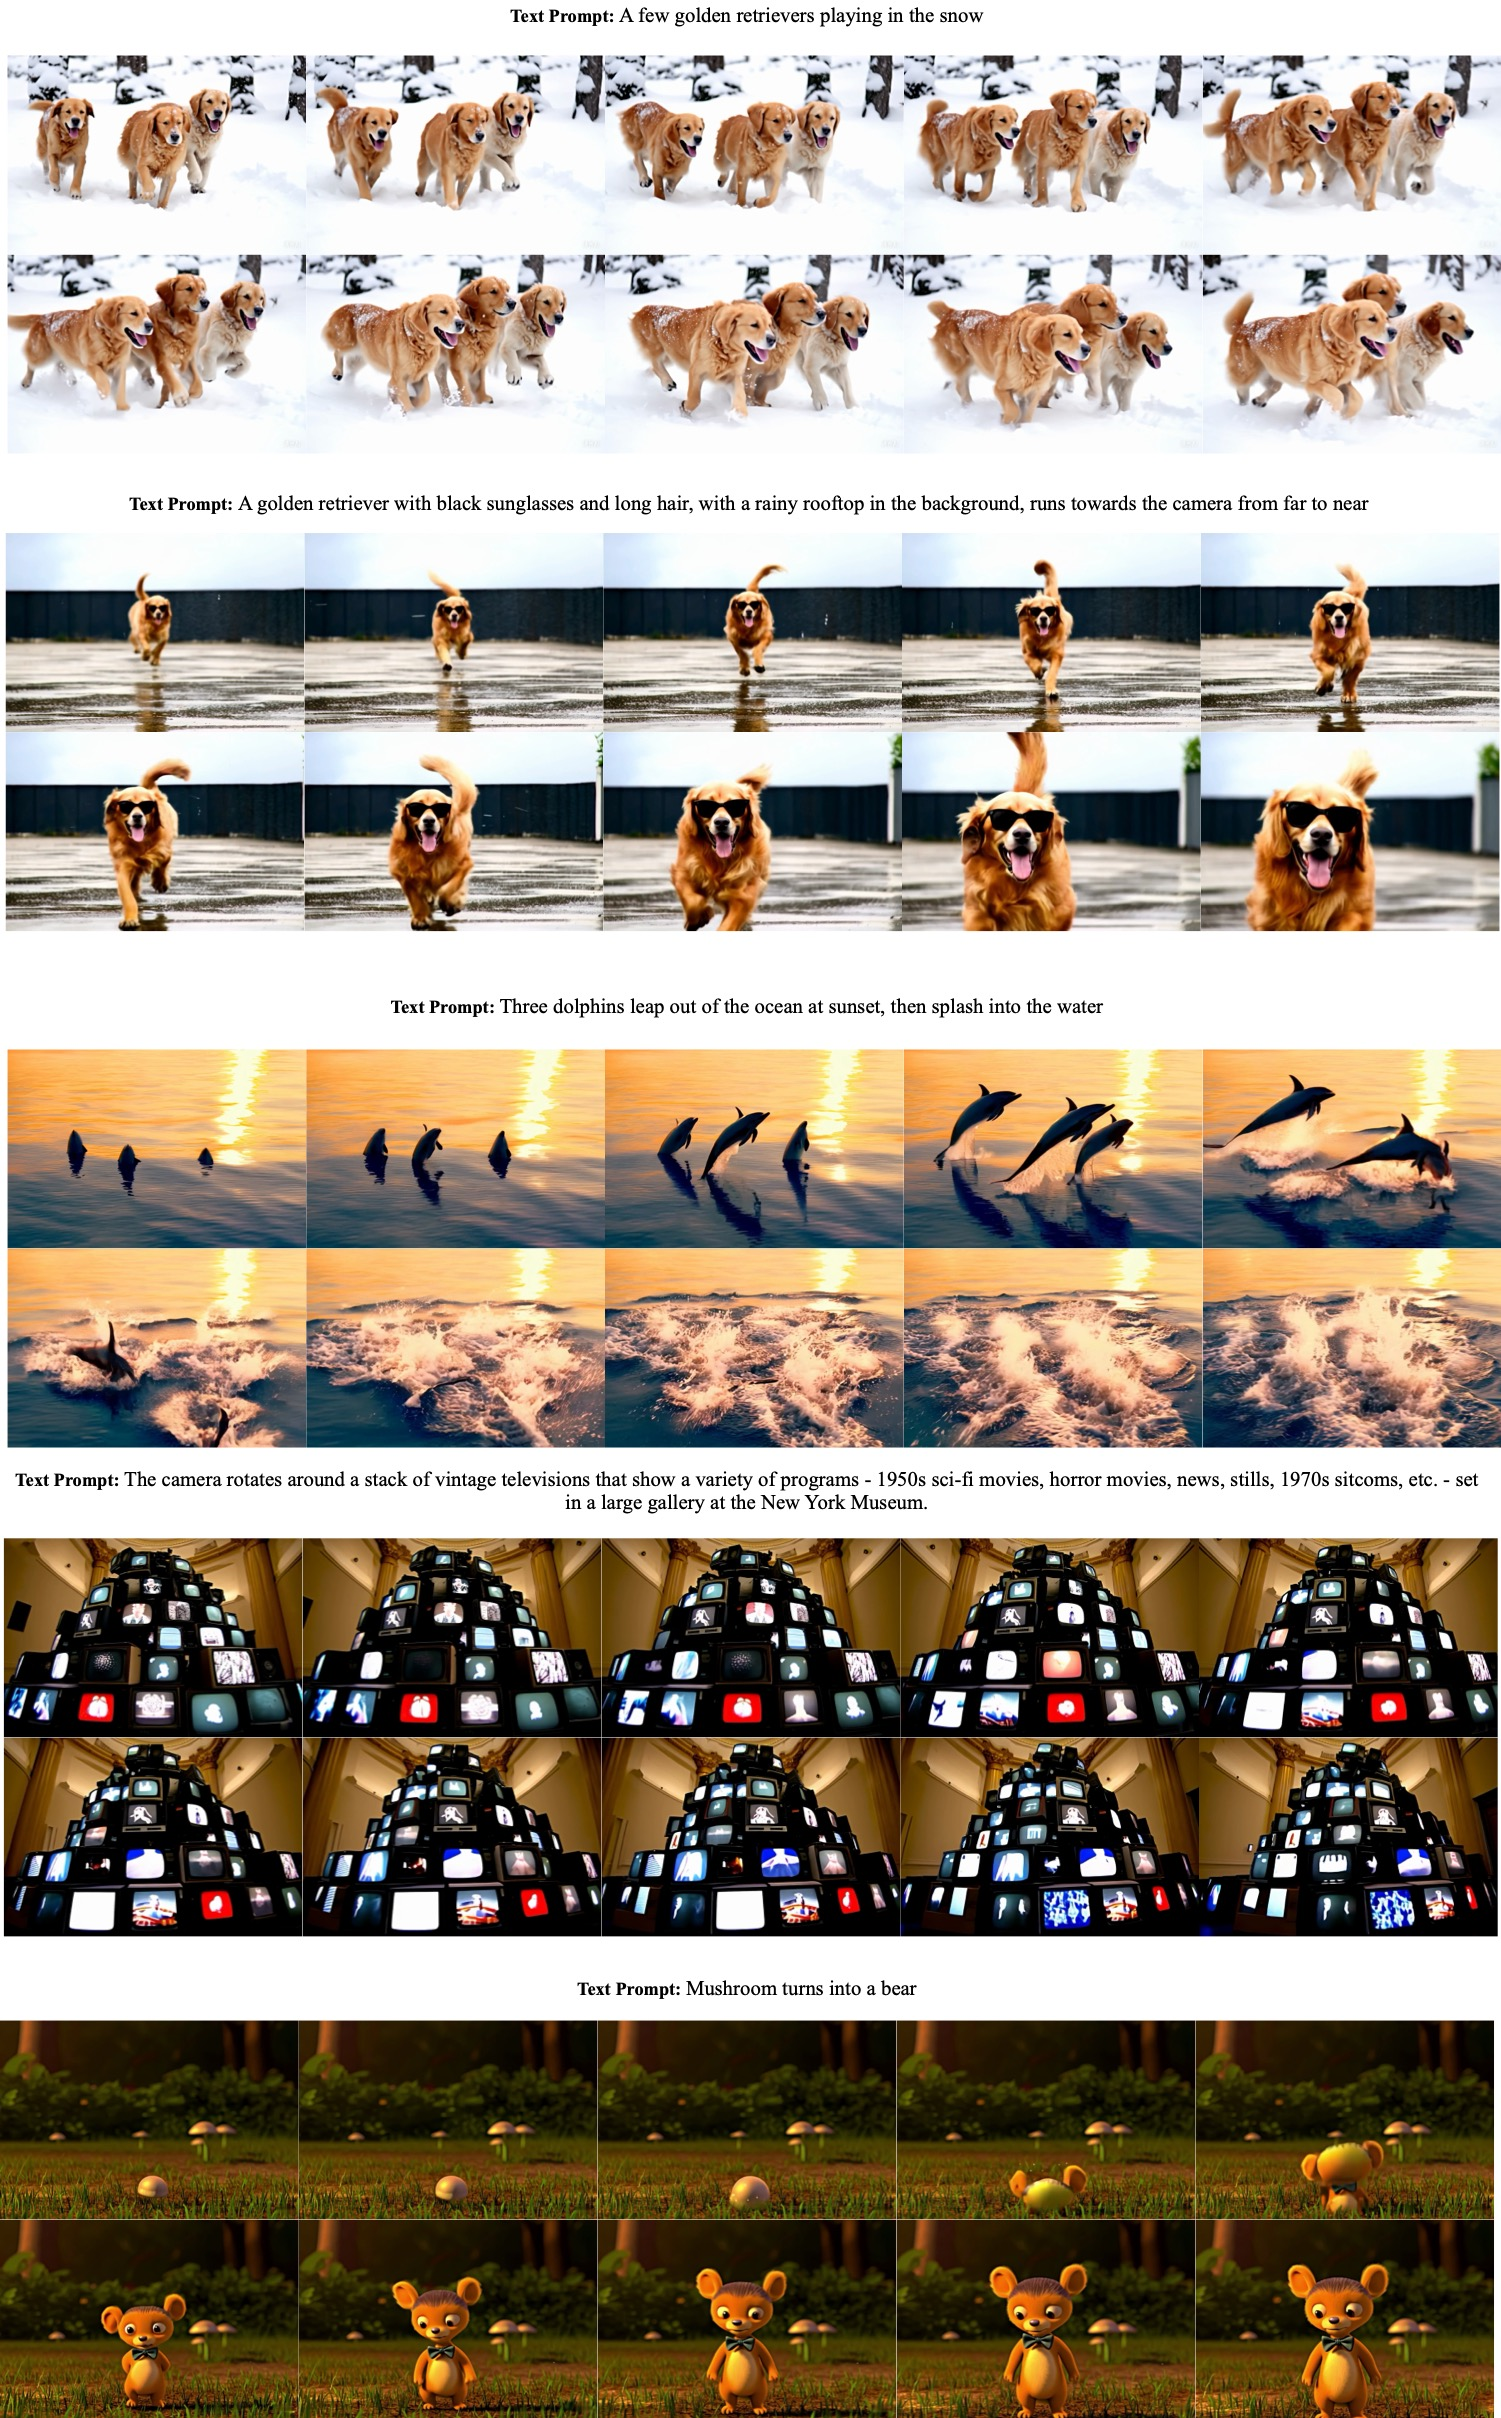
\includegraphics[width=\linewidth]{images/goodcase3.jpg}
\end{center}
\caption{Text to video showcases. The displayed prompt will be upsampled before being fed into the model. The generated videos contain large motion and various styles.}
\label{fig:t2vgood1}
\end{figure}

\begin{figure}[ht]
\vspace{-0.5em}
\begin{center}
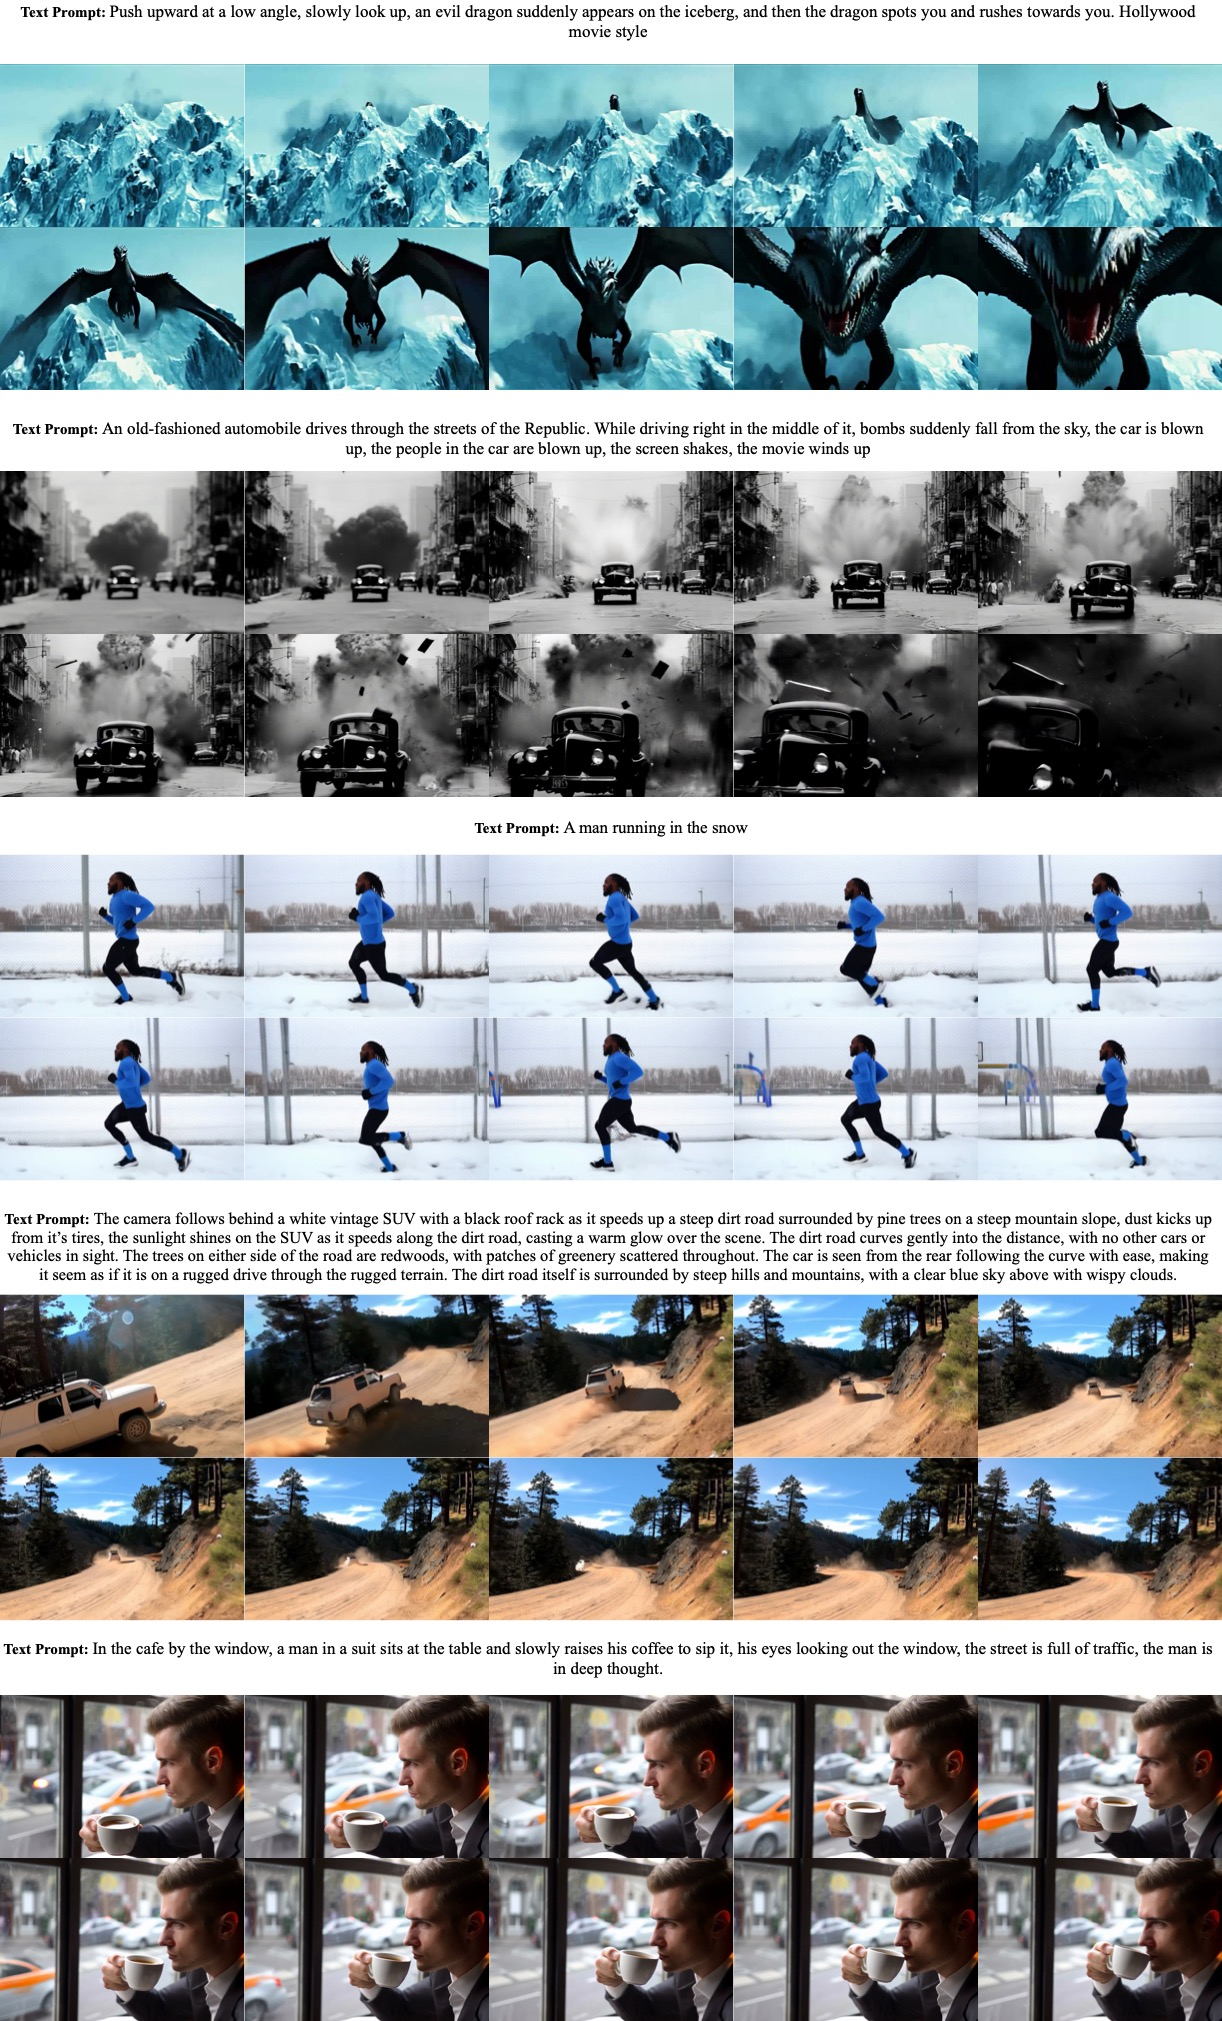
\includegraphics[width=0.98\linewidth]{images/t2v/goodcase2.jpg}
\end{center}
\vspace{-0.5em}
\caption{Text to video showcases.}
\label{fig:t2vgood2}
\end{figure}

\section{Image To Video Model} \label{app:i2v}
We finetune an image-to-video model from the text-to-video model. Drawing from the \citep{blattmann2023stable}, we add an image as an additional condition alongside the text. The image is passed through 3D VAE and concatenated with the noised input in the channel dimension. Similar to super-resolution tasks, there is a significant distribution gap between training and inference (the first frame of videos vs. real-world images). To enhance the model's robustness, we add large noise to the image condition during training. Some examples are shown in Figure~\ref{fig:i2vgood1}, Figure~\ref{fig:i2vgood2}. CogVideoX can handle different styles of image input.

\begin{figure}[ht]
\begin{center}
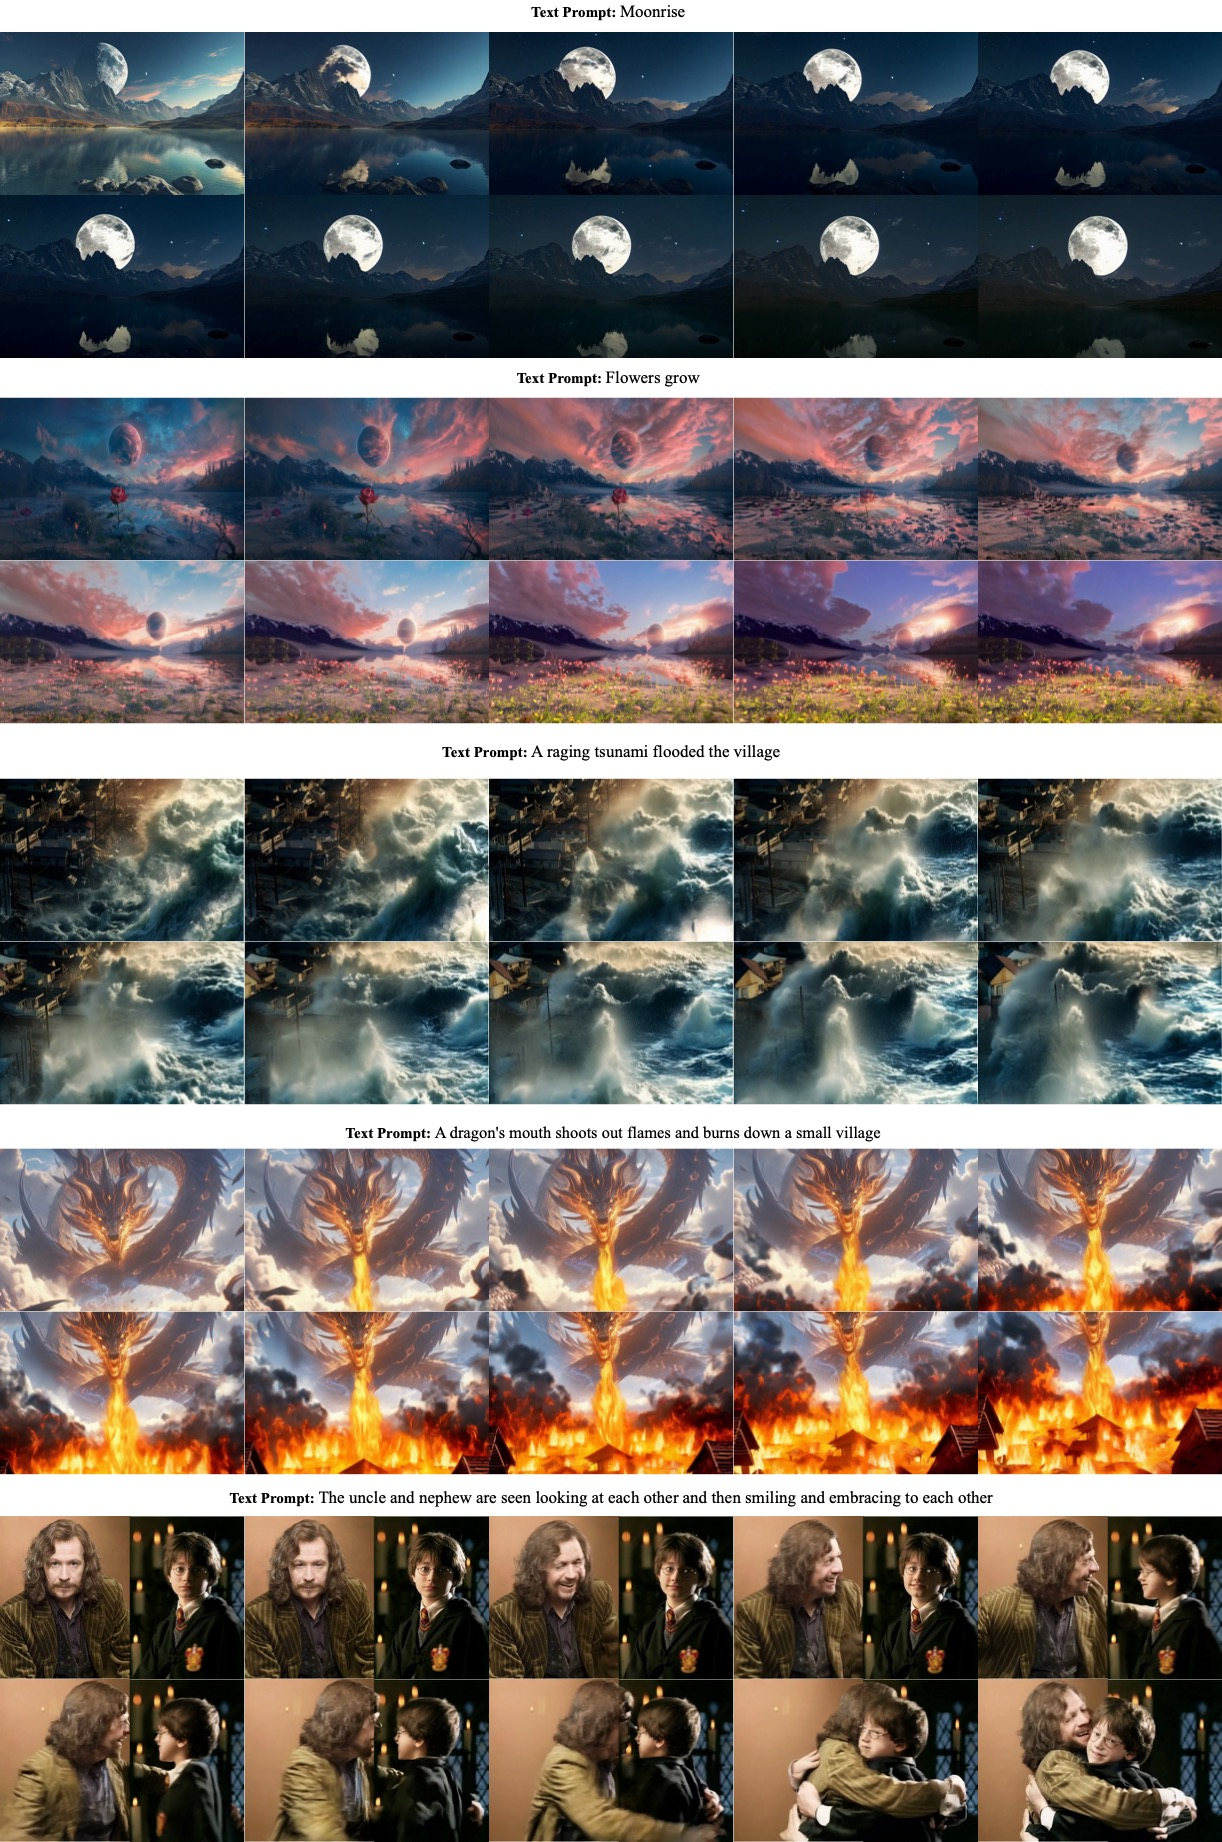
\includegraphics[width=\linewidth]{images/t2v/i2vgood1.jpg}
\end{center}
\caption{Image to video showcases. The displayed prompt will be upsampled before being fed into the model.}
\label{fig:i2vgood1}
\end{figure}

\begin{figure}[ht]
\begin{center}
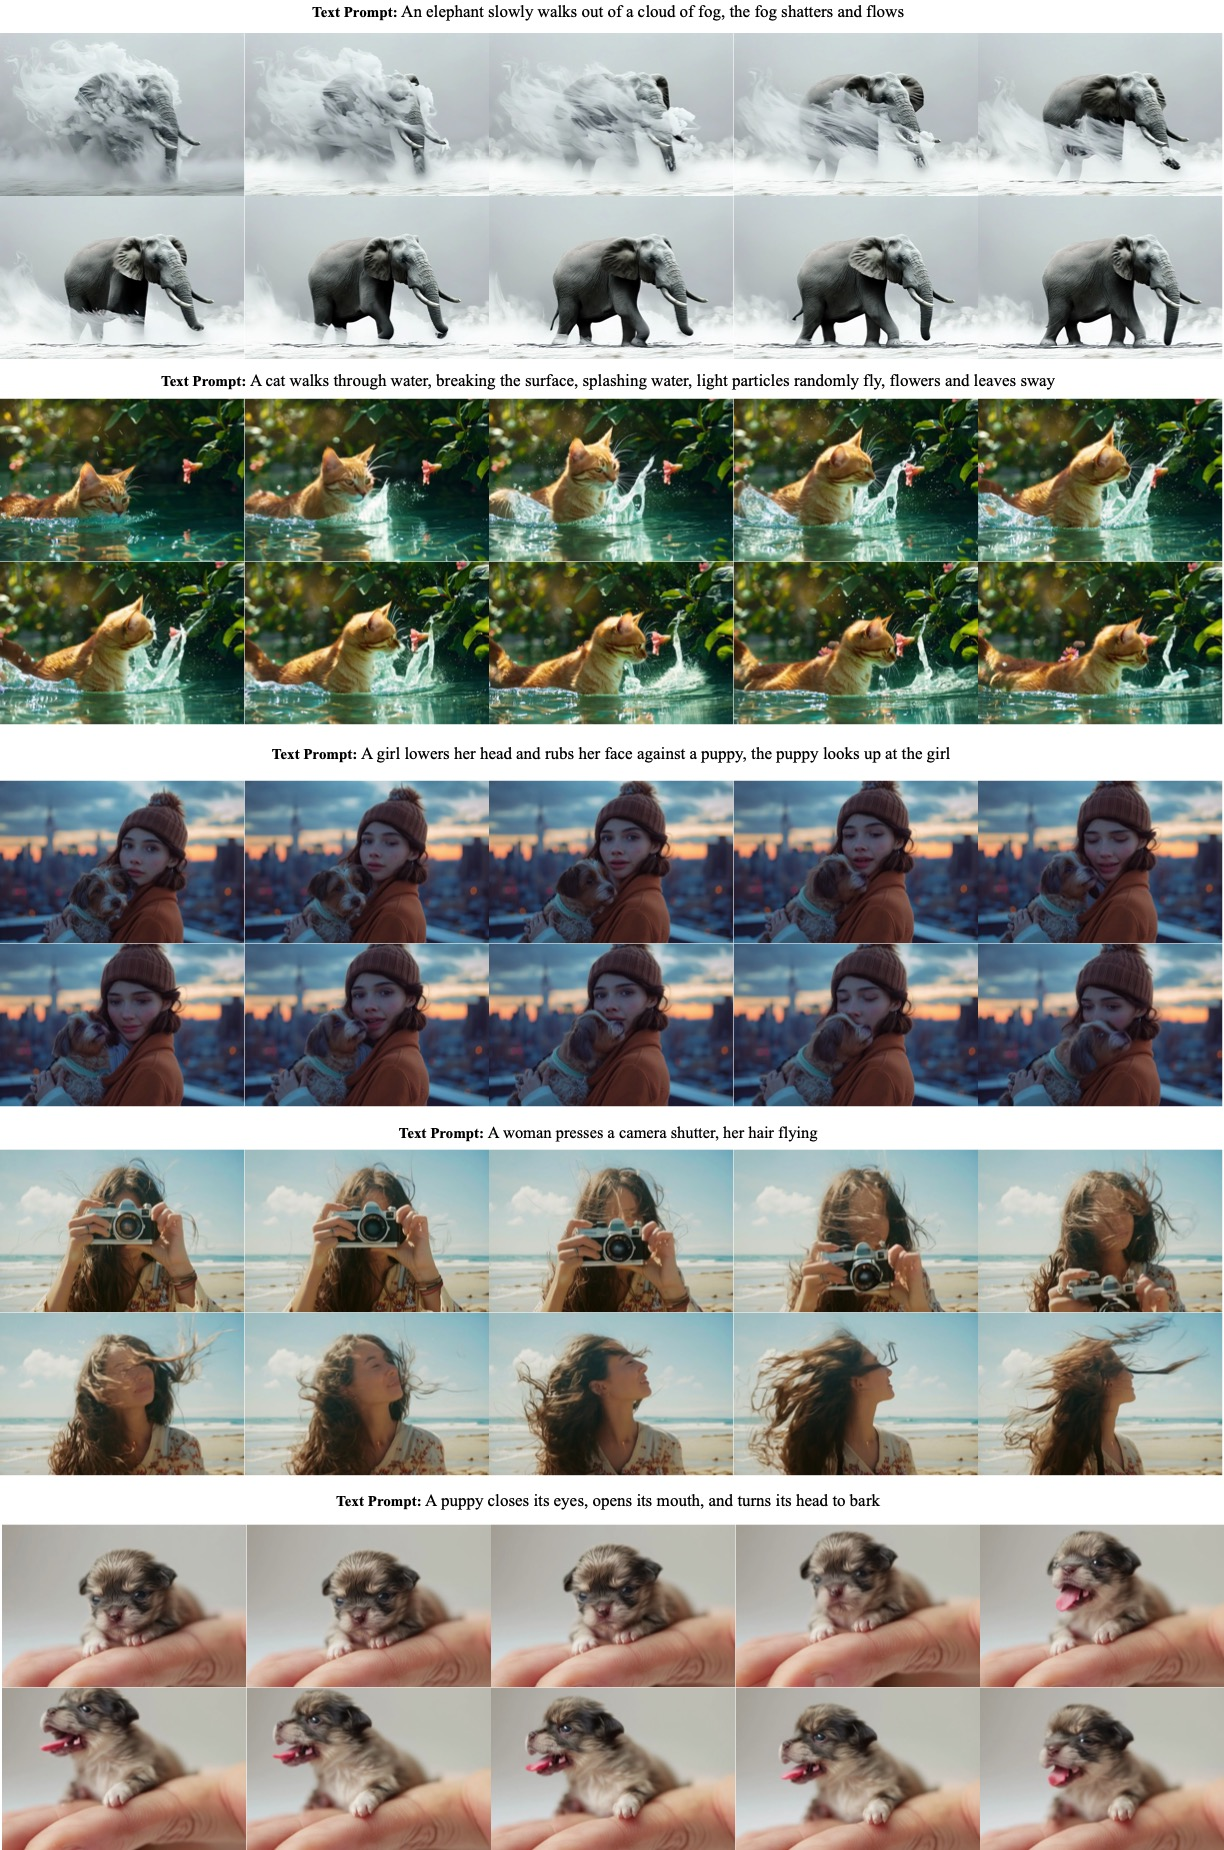
\includegraphics[width=\linewidth]{images/t2v/i2vgood2.jpg}
\end{center}
\caption{Image to video showcases.}
\label{fig:i2vgood2}
\end{figure}
\clearpage
\section{Caption Upsampler}
\label{ap:caption_upsampler}
To ensure that text input distribution during inference is as close as possible to the distribution during training, similar to \citep{betker2023improving}, we use a large language model to upsample the user's input during inference, making it more detailed and precise. Finetuned LLM can generate better prompts than zero/few-shot.

For image-to-video, we use the vision language model to upsample the prompt, such as GPT4V, CogVLM\citep{wang2023cogvlm}. 
\begin{promptbox}[Zero-shot prompt for Text Upsampler]
\noindent
\begin{verbatim}
You are part of a team of bots that create videos. You work 
with an assistant bot that will draw anything you say in 
square brackets. For example, outputting \" a beautiful 
morning in the woods with the sun peaking through the 
trees \" will trigger your partner bot to output a video
of a forest morning, as described. You will be prompted 
by people looking to create detailed, amazing videos. 
The way to accomplish this is to take their short prompts
and make them extremely detailed and descriptive.
There are a few rules to follow :
You will only ever output a single video description 
per user request.
When modifications are requested, you should not simply
make the description longer. You should refactor the
entire description to integrate the suggestions.

\end{verbatim}
\end{promptbox}


\section{Dense Video Caption Data Generation}
\label{ap:video_caption_gen}

In the pipeline for generating video captions, we extract one frame every two seconds for image captioning. Ultimately, we collected 50,000 data points to fine-tune the summary model. Below is the prompt we used for summarization with GPT-4:
\begin{promptbox}[Prompt for GPT-4 Summary]
\noindent
\begin{verbatim}
We extracted several frames from this video and described 
each frame using an image understanding model,  stored 
in the dictionary variable `image_captions: Dict[str: str]`.  
In `image_captions`,  the key is the second at which the image 
appears in the  video,  and the value is a detailed description 
of the image at that moment. Please describe the content of 
this video  in as much detail as possible,  based on the 
information  provided by `image_captions`,  including 
the objects, scenery, animals, characters, and camera 
movements within the video. \n image_captions={new_captions}\n 
You should output your summary directly,  and not mention
variables like `image_captions` in your response. 
Do not include `\\n' and the word 'video' in your response.  
Do not use introductory phrases such as: \"The video 
presents\", \"The video depicts\", \"This video showcases\", 
\"The video captures\" and so on.\n Please start the 
description with the video content directly, such as \"A man
first sits in a chair, then stands up and walks to the 
kitchen....\"\n Do not use phrases like: \"as the video 
progressed\" and \"Throughout the video\".\n Please describe 
the content of the video and the changes that occur, in 
chronological order.\n Please keep the description of this 
video within 100 English words.
\end{verbatim}
\end{promptbox}


\section{Video Caption Example}
\label{ap:video_caption_example}


Below we present more examples to compare the performance of the Panda-70M video captioning model and our CogVLM2-Caption model:

\begin{figure}[h]
\begin{center}
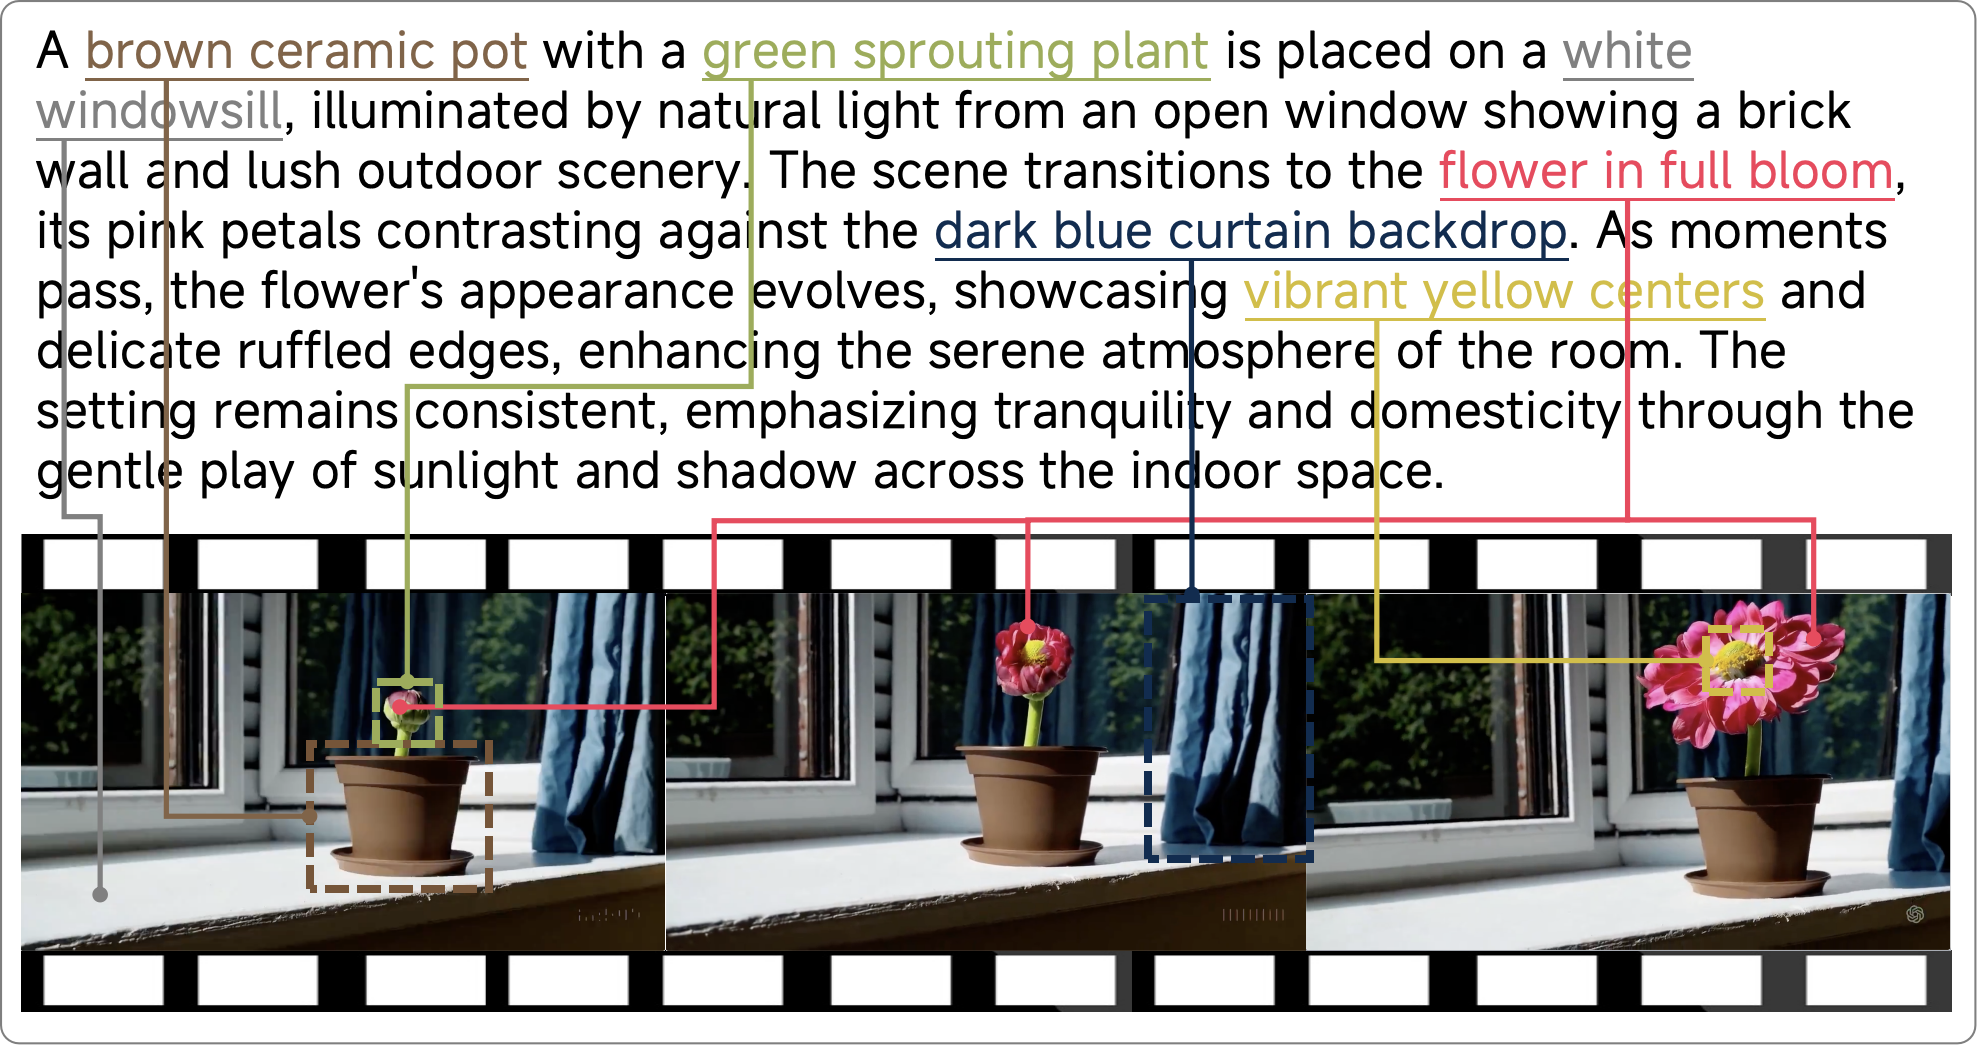
\includegraphics[width=0.9\linewidth]{images/v2t/detail_example.png}
\end{center}
\caption{An example from CogVLM2-Caption provides a detailed description of all specific objects and movements.}
\label{fig:v2t}
\end{figure}

% \begin{figure}[h]
\begin{center}
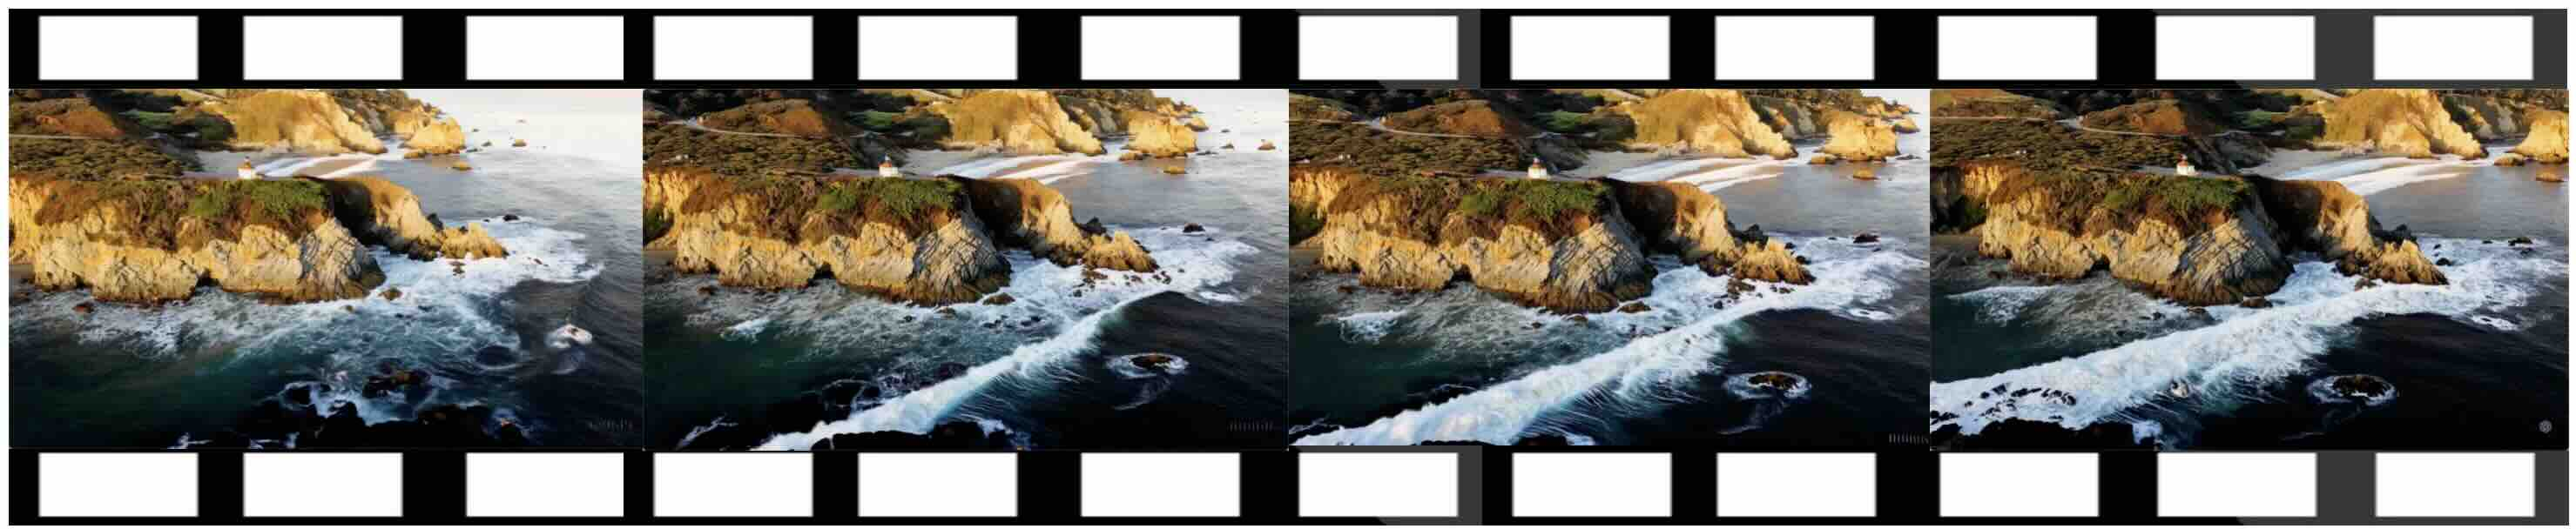
\includegraphics[width=0.9\linewidth]{images/caption_example1.jpg}
\end{center}
\end{figure}
% \begin{promptbox}[Caption Generated by Panda-70M]
% \begin{verbatim}
% There is an aerial view of a rocky coastline with waves 
% crashing against the shore, and a lighthouse on a cliff.
% \end{verbatim}
% \end{promptbox}
% \begin{promptbox}[Caption Generated by CogVLM2-Caption]
% \begin{verbatim}
% The video features a rugged coastline with cliffs descending 
% into the sea, where waves crash against rocks. A lighthouse 
% stands on a promontory, surrounded by greenery and bathed in
% sunlight that casts long shadows. The scene is tranquil yet 
% dynamic, with no human presence initially. As time passes, a 
% solitary house appears atop an elevated cliff, overlooking the 
% ocean. The landscape's colors transition from deep blues to 
% golden hues, suggesting dawn or dusk. Eventually, a road winds
% along the coast, leading to the secluded beach and lighthouse, 
% emphasizing the area's serene isolation amidst nature's 
% grandeur.
% \end{verbatim}
% \end{promptbox}


% \begin{figure}[h]
\begin{center}
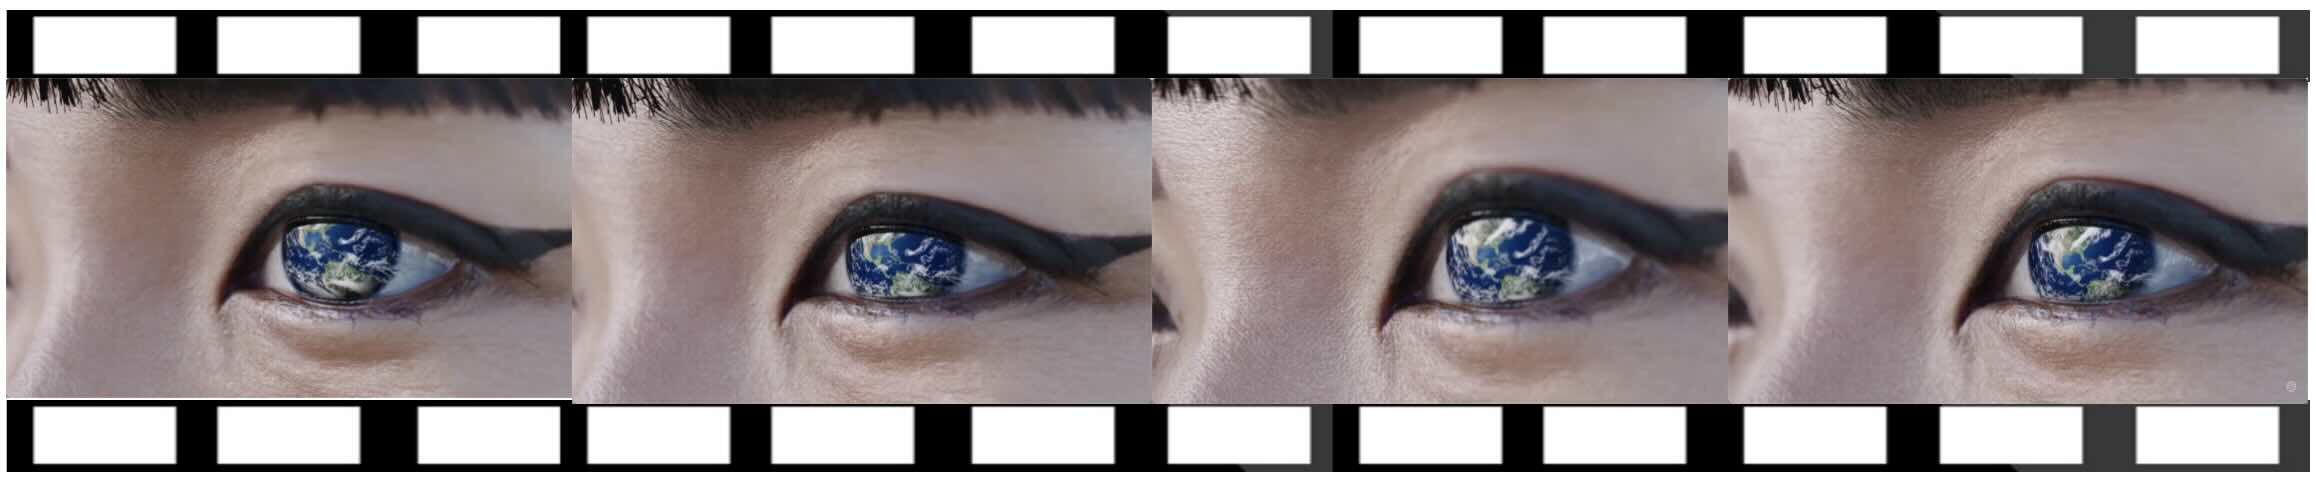
\includegraphics[width=0.9\linewidth]{images/caption_example2.jpg}
\end{center}
\end{figure}
% \begin{promptbox}[Caption Generated by Panda-70M]
% \begin{verbatim}
% A close up of a woman's eye with the earth in it.
% \end{verbatim}
% \end{promptbox}
% \begin{promptbox}[Caption Generated by CogVLM2-Caption]
% \begin{verbatim}
% A woman's eye, in sharp focus and detailed with a bold black
% eyeliner, reflects the Earth. The vivid colors of blue oceans
% and green continents stand out against her clear iris,
% symbolizing a deep connection between humanity and our planet.
% Her expression remains neutral throughout, emphasizing 
% introspection or awareness. As time passes, the reflection
% subtly shifts to include parts of Africa and Europe, suggesting
% a global perspective. The contrast between her dark eyelashes
% and light skin accentuates the visual metaphor for unity and 
% interconnectedness, while her gaze suggests contemplation on
% environmental issues or a profound sense of responsibility
% towards the world.
% \end{verbatim}
% \end{promptbox}


\begin{figure}[h]
\begin{center}
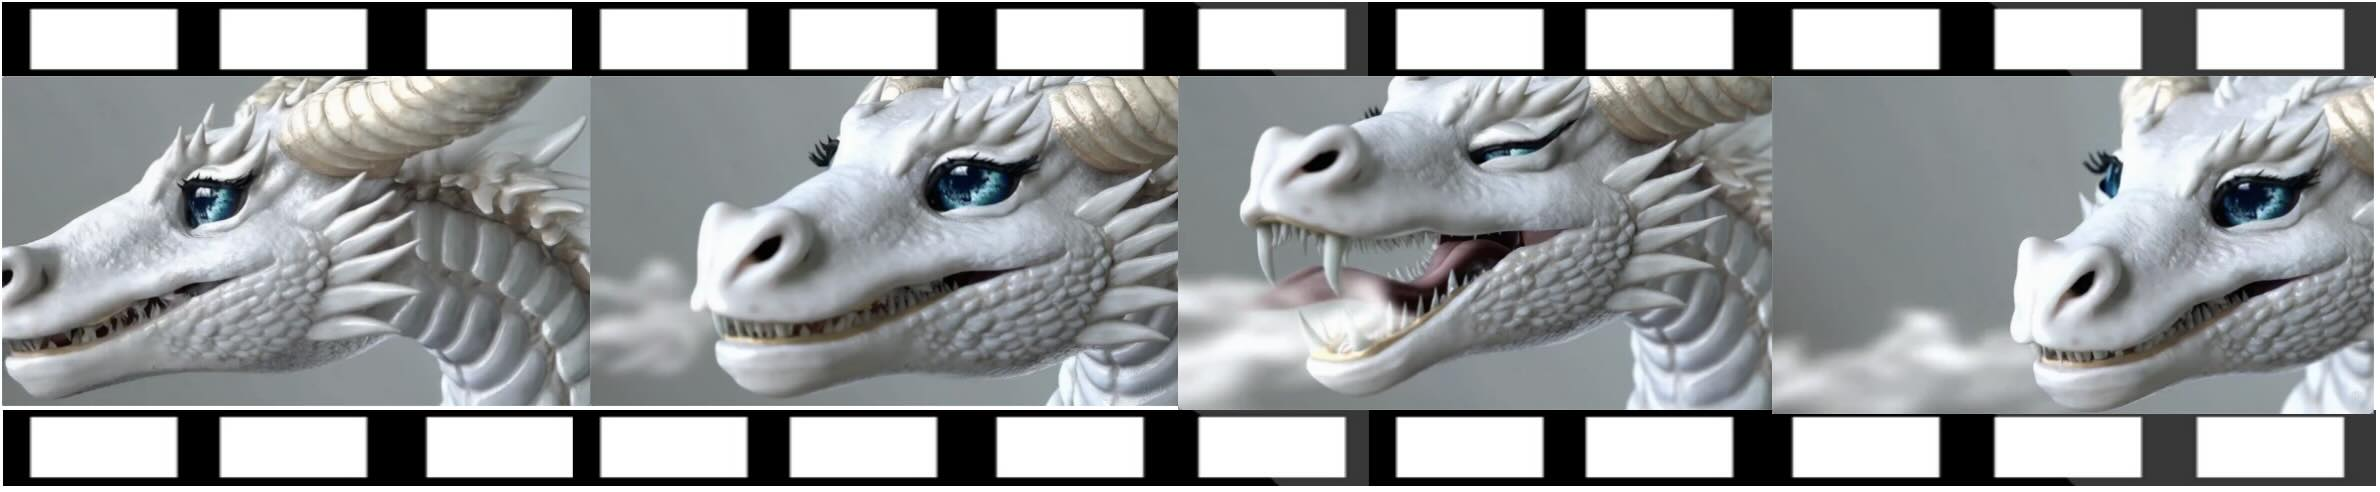
\includegraphics[width=0.9\linewidth]{images/caption_example3.jpg}
\end{center}
\end{figure}
\begin{promptbox}[Caption Generated by Panda-70M]
\begin{verbatim}
A close up of a white dragon with blue eyes.
\end{verbatim}
\end{promptbox}
\begin{promptbox}[Caption Generated by CogVLM2-Caption]
\begin{verbatim}
A meticulously crafted white dragon with a serene expression 
and piercing blue eyes is showcased in various close-ups, its 
scales detailed with golden highlights. Initially, the dragon's
horns are curved back, but as time passes, they change to 
spiraling gold, adding elegance. The creature's demeanor shifts 
from tranquil majesty to a more formidable presence, with its 
mouth agape revealing sharp teeth at times. Its expressions 
alternate between calmness and fierce determination, 
maintaining an air of mythical serenity throughout. The 
consistent neutral background focuses attention on the dragon's
textured features and expressive eyes.
\end{verbatim}
\end{promptbox}


\begin{figure}[h]
\begin{center}
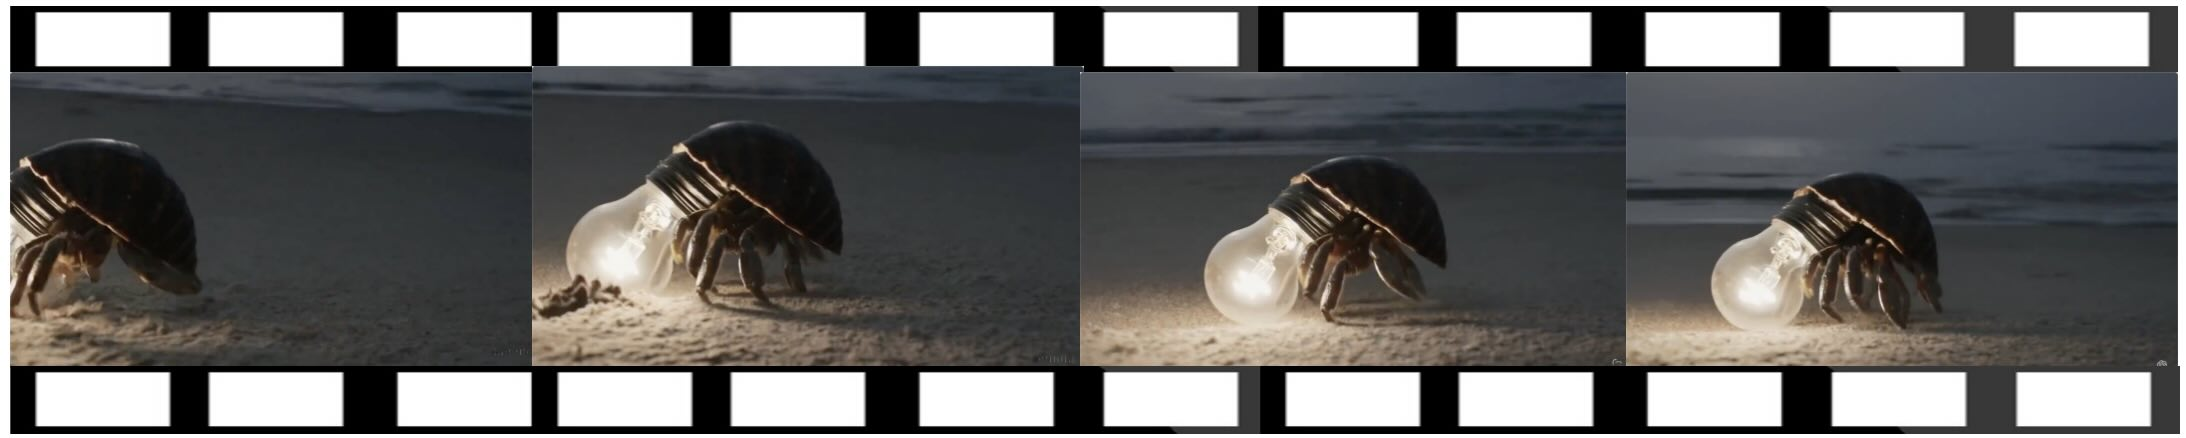
\includegraphics[width=0.9\linewidth]{images/caption_example4.jpg}
\end{center}
\end{figure}
\begin{promptbox}[Caption Generated by Panda-70M]
\begin{verbatim}
A crab is walking on the beach with a light bulb on its back.
\end{verbatim}
\end{promptbox}
\begin{promptbox}[Caption Generated by CogVLM2-Caption]
\begin{verbatim}
A hermit crab with a dark, glossy shell and reddish-brown legs
is seen carrying an illuminated light bulb on its back across 
the sandy terrain of a beach at night. The scene transitions 
from a soft glow to a more pronounced illumination as the crab
moves, highlighting its delicate limbs against the smooth sand
and tranquil sea backdrop. This surreal tableau blends natural
beauty with human ingenuity, creating a serene yet whimsical 
atmosphere that emphasizes the crab's unique adaptation and the
contrast between nature and technology in this quiet nocturnal
setting.
\end{verbatim}
\end{promptbox}


\begin{figure}[h]
\begin{center}
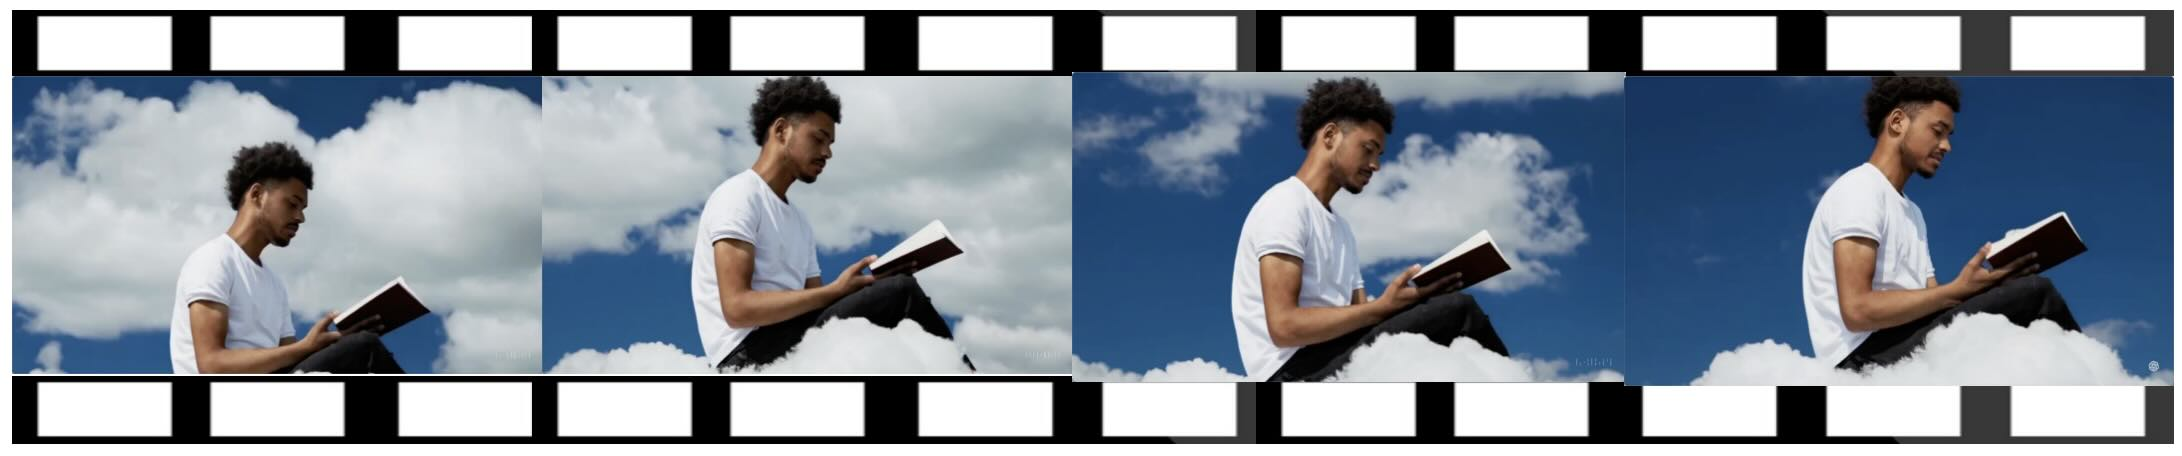
\includegraphics[width=0.9\linewidth]{images/caption_example5.jpg}
\end{center}
\end{figure}
\begin{promptbox}[Caption Generated by Panda-70M]
\begin{verbatim}
A young black man is sitting on a cloud and reading a book 
with a blue sky in the background.
\end{verbatim}
\end{promptbox}
\begin{promptbox}[Caption Generated by CogVLM2-Caption]
\begin{verbatim}
A young Black man with an afro hairstyle and a neatly trimmed 
beard is seen sitting cross-legged on fluffy white clouds, 
deeply engrossed in reading a book with a red cover. He wears 
a plain white T-shirt and dark pants against a vivid blue sky 
dotted with cumulus clouds. Throughout the scenes, his 
expression remains one of deep concentration and peaceful 
contemplation, highlighting a moment of intellectual pursuit 
amidst nature's grandeur. The imagery suggests a serene 
atmosphere that emphasizes solitude and introspection, with no 
other people or objects around him.
\end{verbatim}
\end{promptbox}


% \begin{figure}[h]
\begin{center}
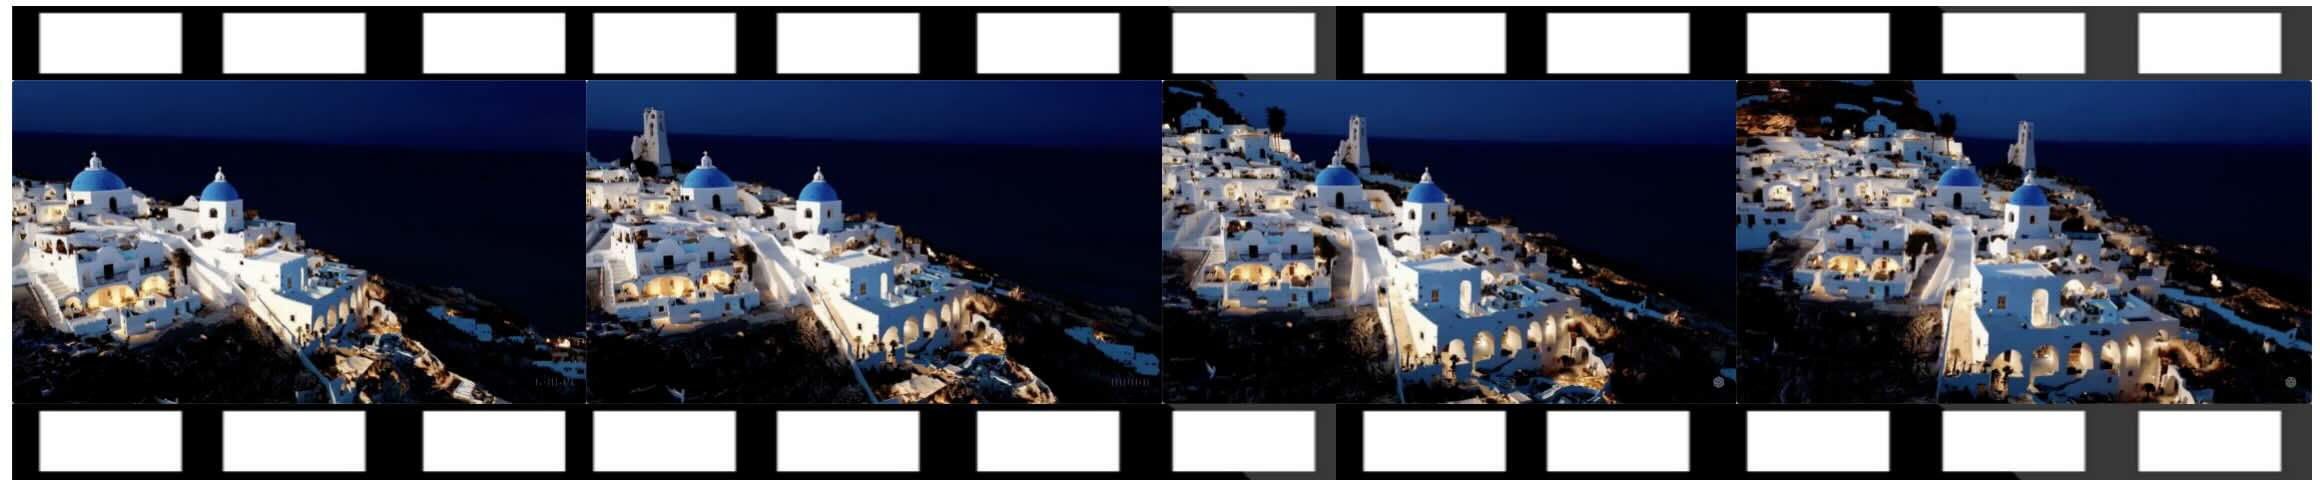
\includegraphics[width=0.9\linewidth]{images/caption_example6.jpg}
\end{center}
\end{figure}
% \begin{promptbox}[Caption Generated by Panda-70M]
% \begin{verbatim}
% A white church on a cliff overlooking the ocean at night.
% \end{verbatim}
% \end{promptbox}
% \begin{promptbox}[Caption Generated by CogVLM2-Caption]
% \begin{verbatim}
% A picturesque evening descends on a cliffside village, 
% showcasing whitewashed buildings with blue domes that glow 
% against the darkening sky. The Aegean Sea mirrors this 
% celestial hue, creating a serene tableau devoid of people and 
% vehicles. As time passes, the scene remains tranquil, 
% illuminated by golden lights from within homes and lit 
% pathways weaving between structures. A solitary windmill 
% stands out, symbolizing local culture amidst the peaceful 
% setting. The absence of visible human activity emphasizes the 
% stillness and beauty of the coastal hamlet, inviting 
% contemplation in its embrace.
% \end{verbatim}
% \end{promptbox}


% \begin{figure}[h]
\begin{center}
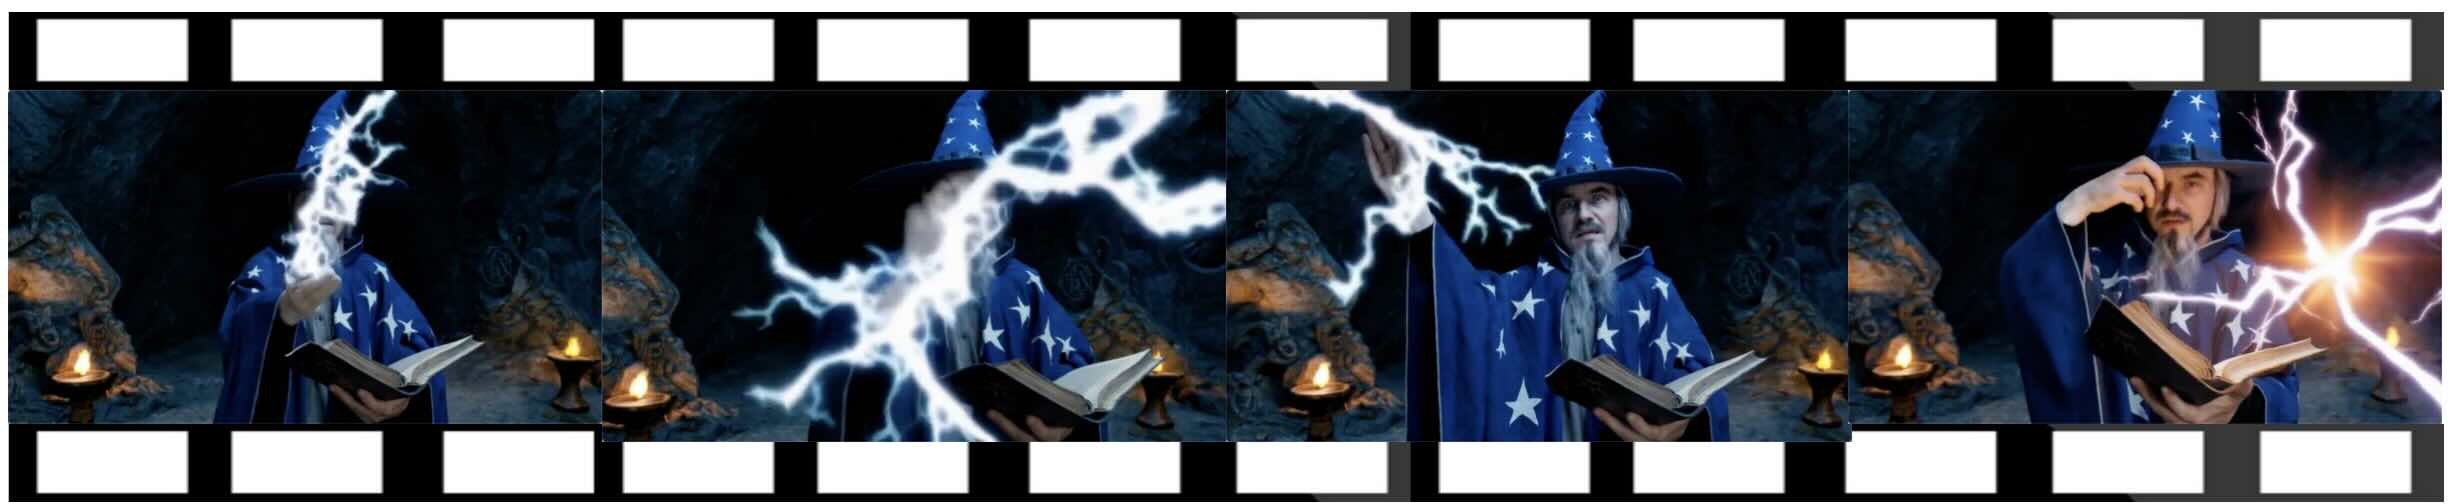
\includegraphics[width=0.9\linewidth]{images/caption_example7.jpg}
\end{center}
\end{figure}
% \begin{promptbox}[Caption Generated by Panda-70M]
% \begin{verbatim}
% A man dressed as a wizard is holding a book and a lightning
% bolt is coming out of it.
% \end{verbatim}
% \end{promptbox}
% \begin{promptbox}[Caption Generated by CogVLM2-Caption]
% \begin{verbatim}
% A man dressed as a wizard, with a blue robe adorned with white
% stars and a matching pointed hat, stands in a dark cave. He is 
% engaged in casting spells from an open book, surrounded by 
% mystical flames that illuminate the scene. Throughout the 
% sequence, his right hand is raised to channel bright lightning
% bolts towards unseen targets, while his left hand holds the
% book firmly. His expression remains focused and serious, 
% suggesting deep concentration on his magical endeavors. The 
% atmosphere of mystery and ancient magic is enhanced by the 
% surrounding darkness and the vivid display of light and shadow.
% \end{verbatim}
% \end{promptbox}
\clearpage
\section{Video to Video via CogVideoX and CogVLM2-Caption}
\label{ap:v2v}

In this section, we present several examples of video-to-video generation using CogVideoX and CogVLM2-Caption. Specifically, we first input the original video into CogVLM2-Caption to obtain the video's caption, and then feed this caption into the CogVideoX model to generate a new video. From the examples below, it can be seen that our pipeline achieves a high degree of fidelity to the original video, showing that CogVLM2-Caption can capture almost all the details in the video.

\begin{figure}[h]
\begin{center}
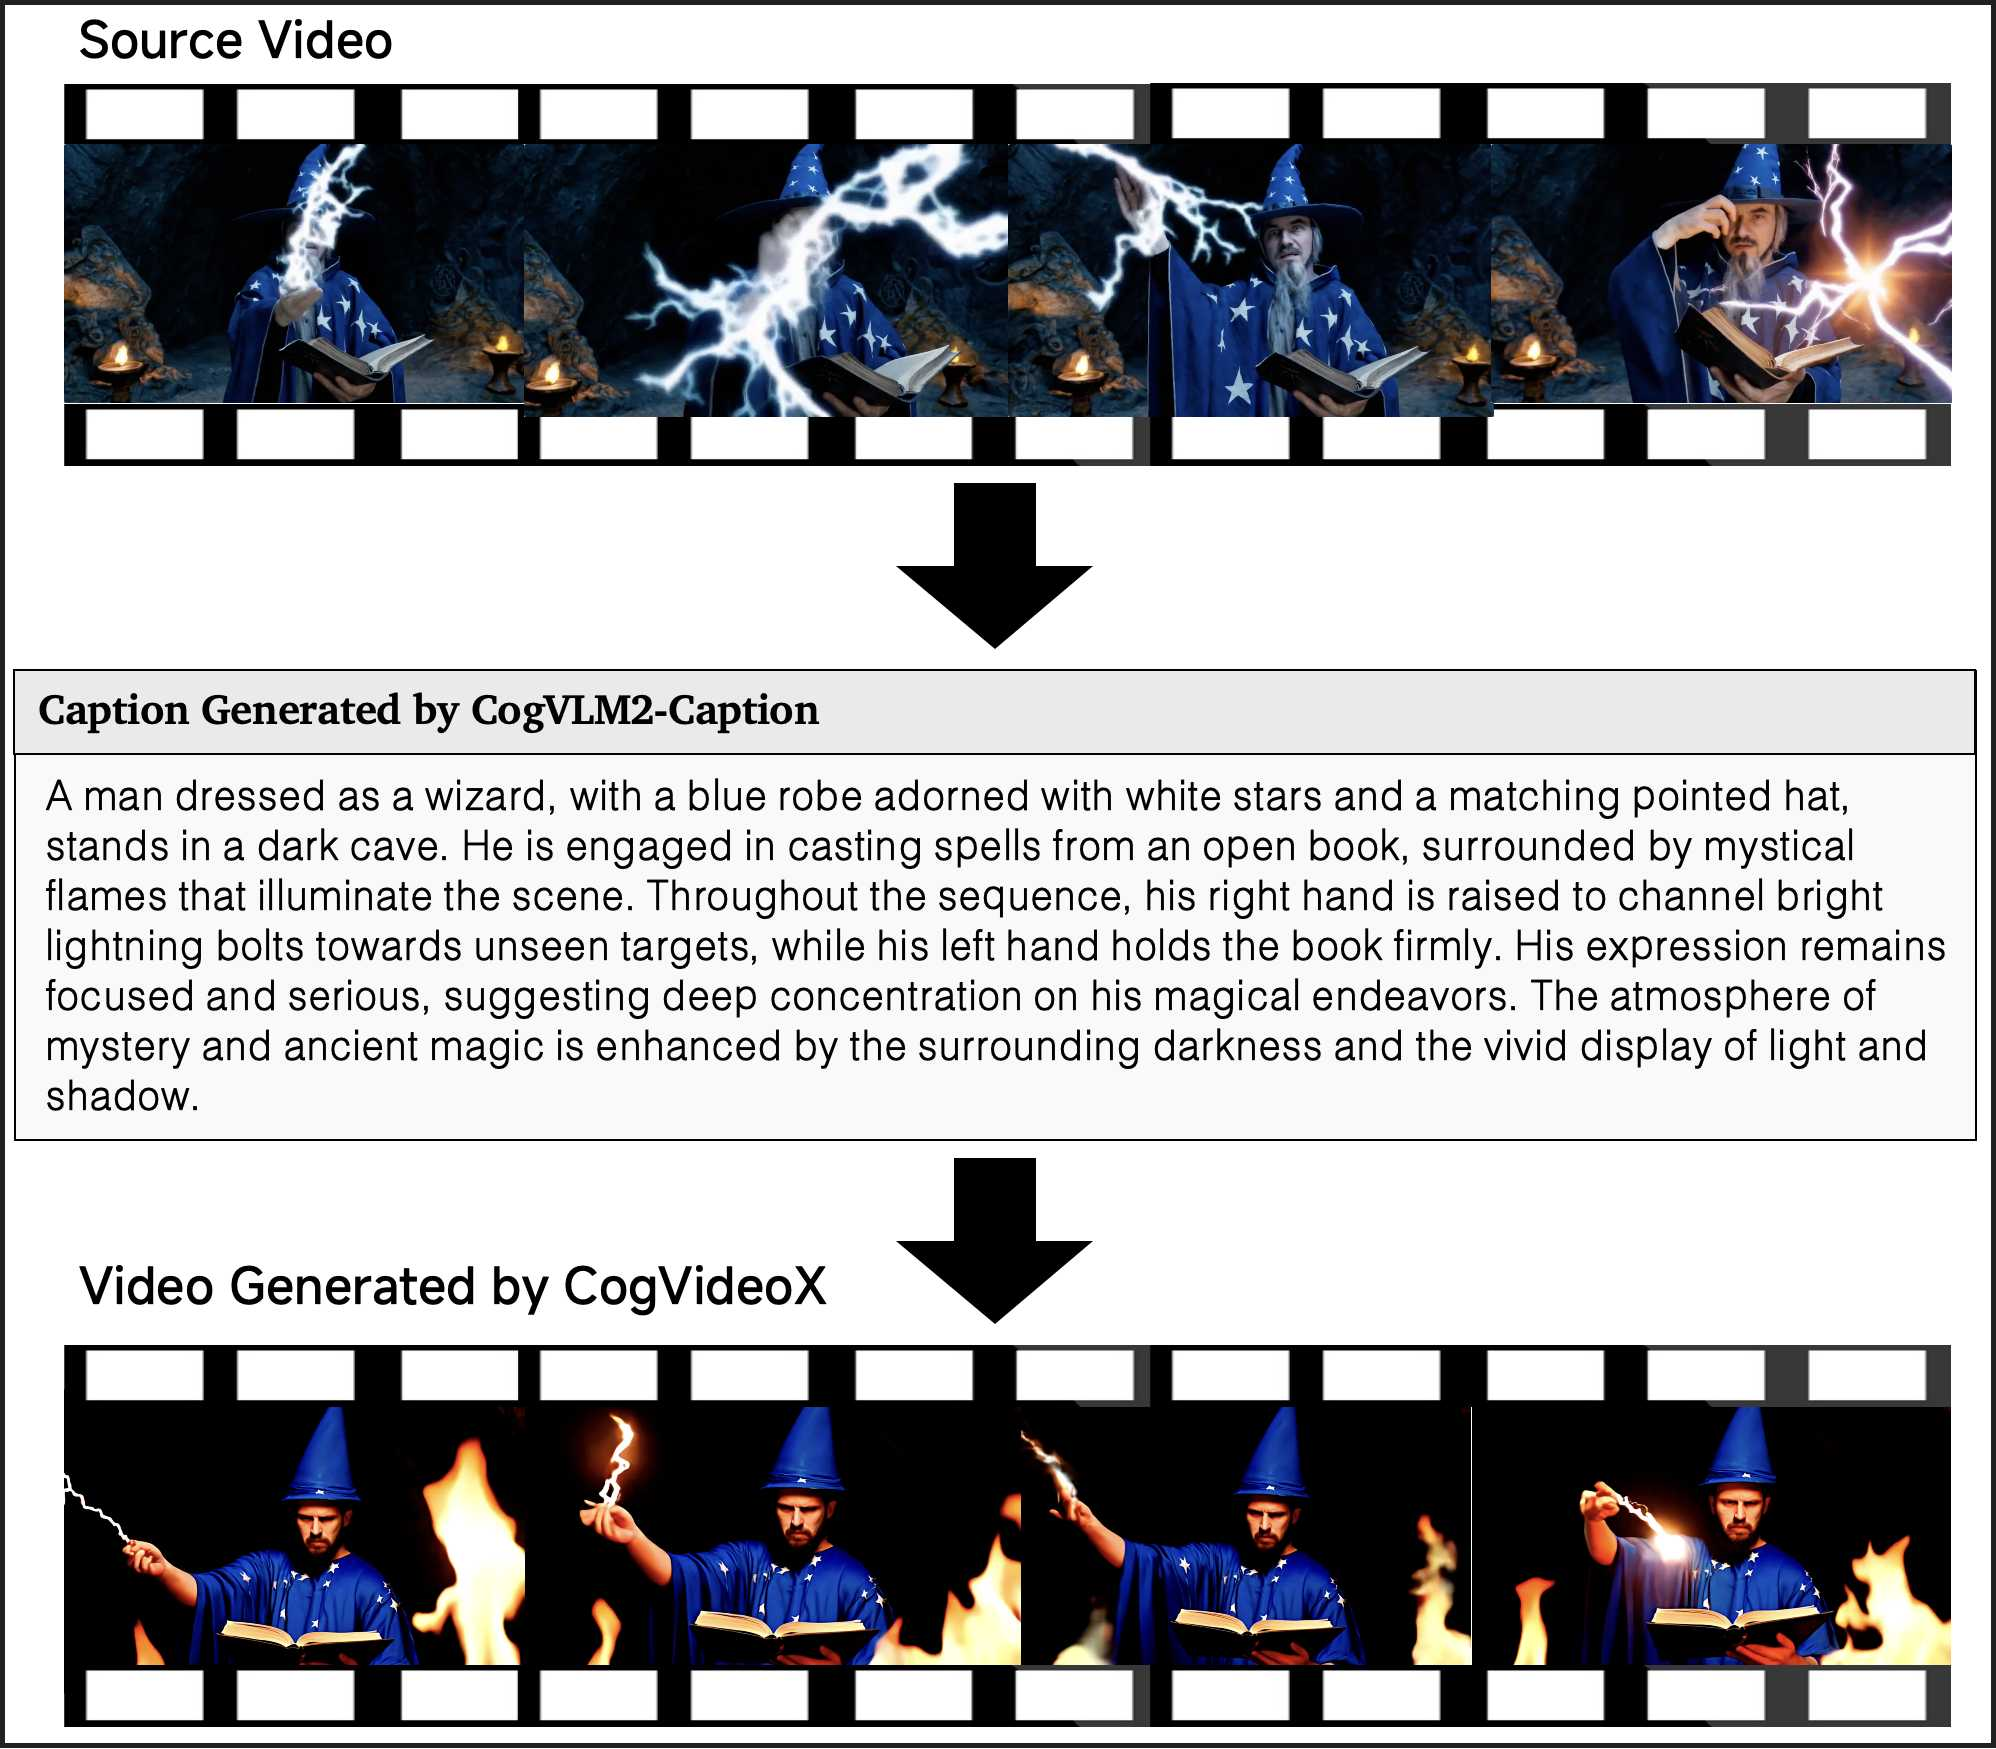
\includegraphics[width=0.9\linewidth]{images/v2v/v2v_1.jpg}
\end{center}
\end{figure}

\begin{figure}[h]
\begin{center}
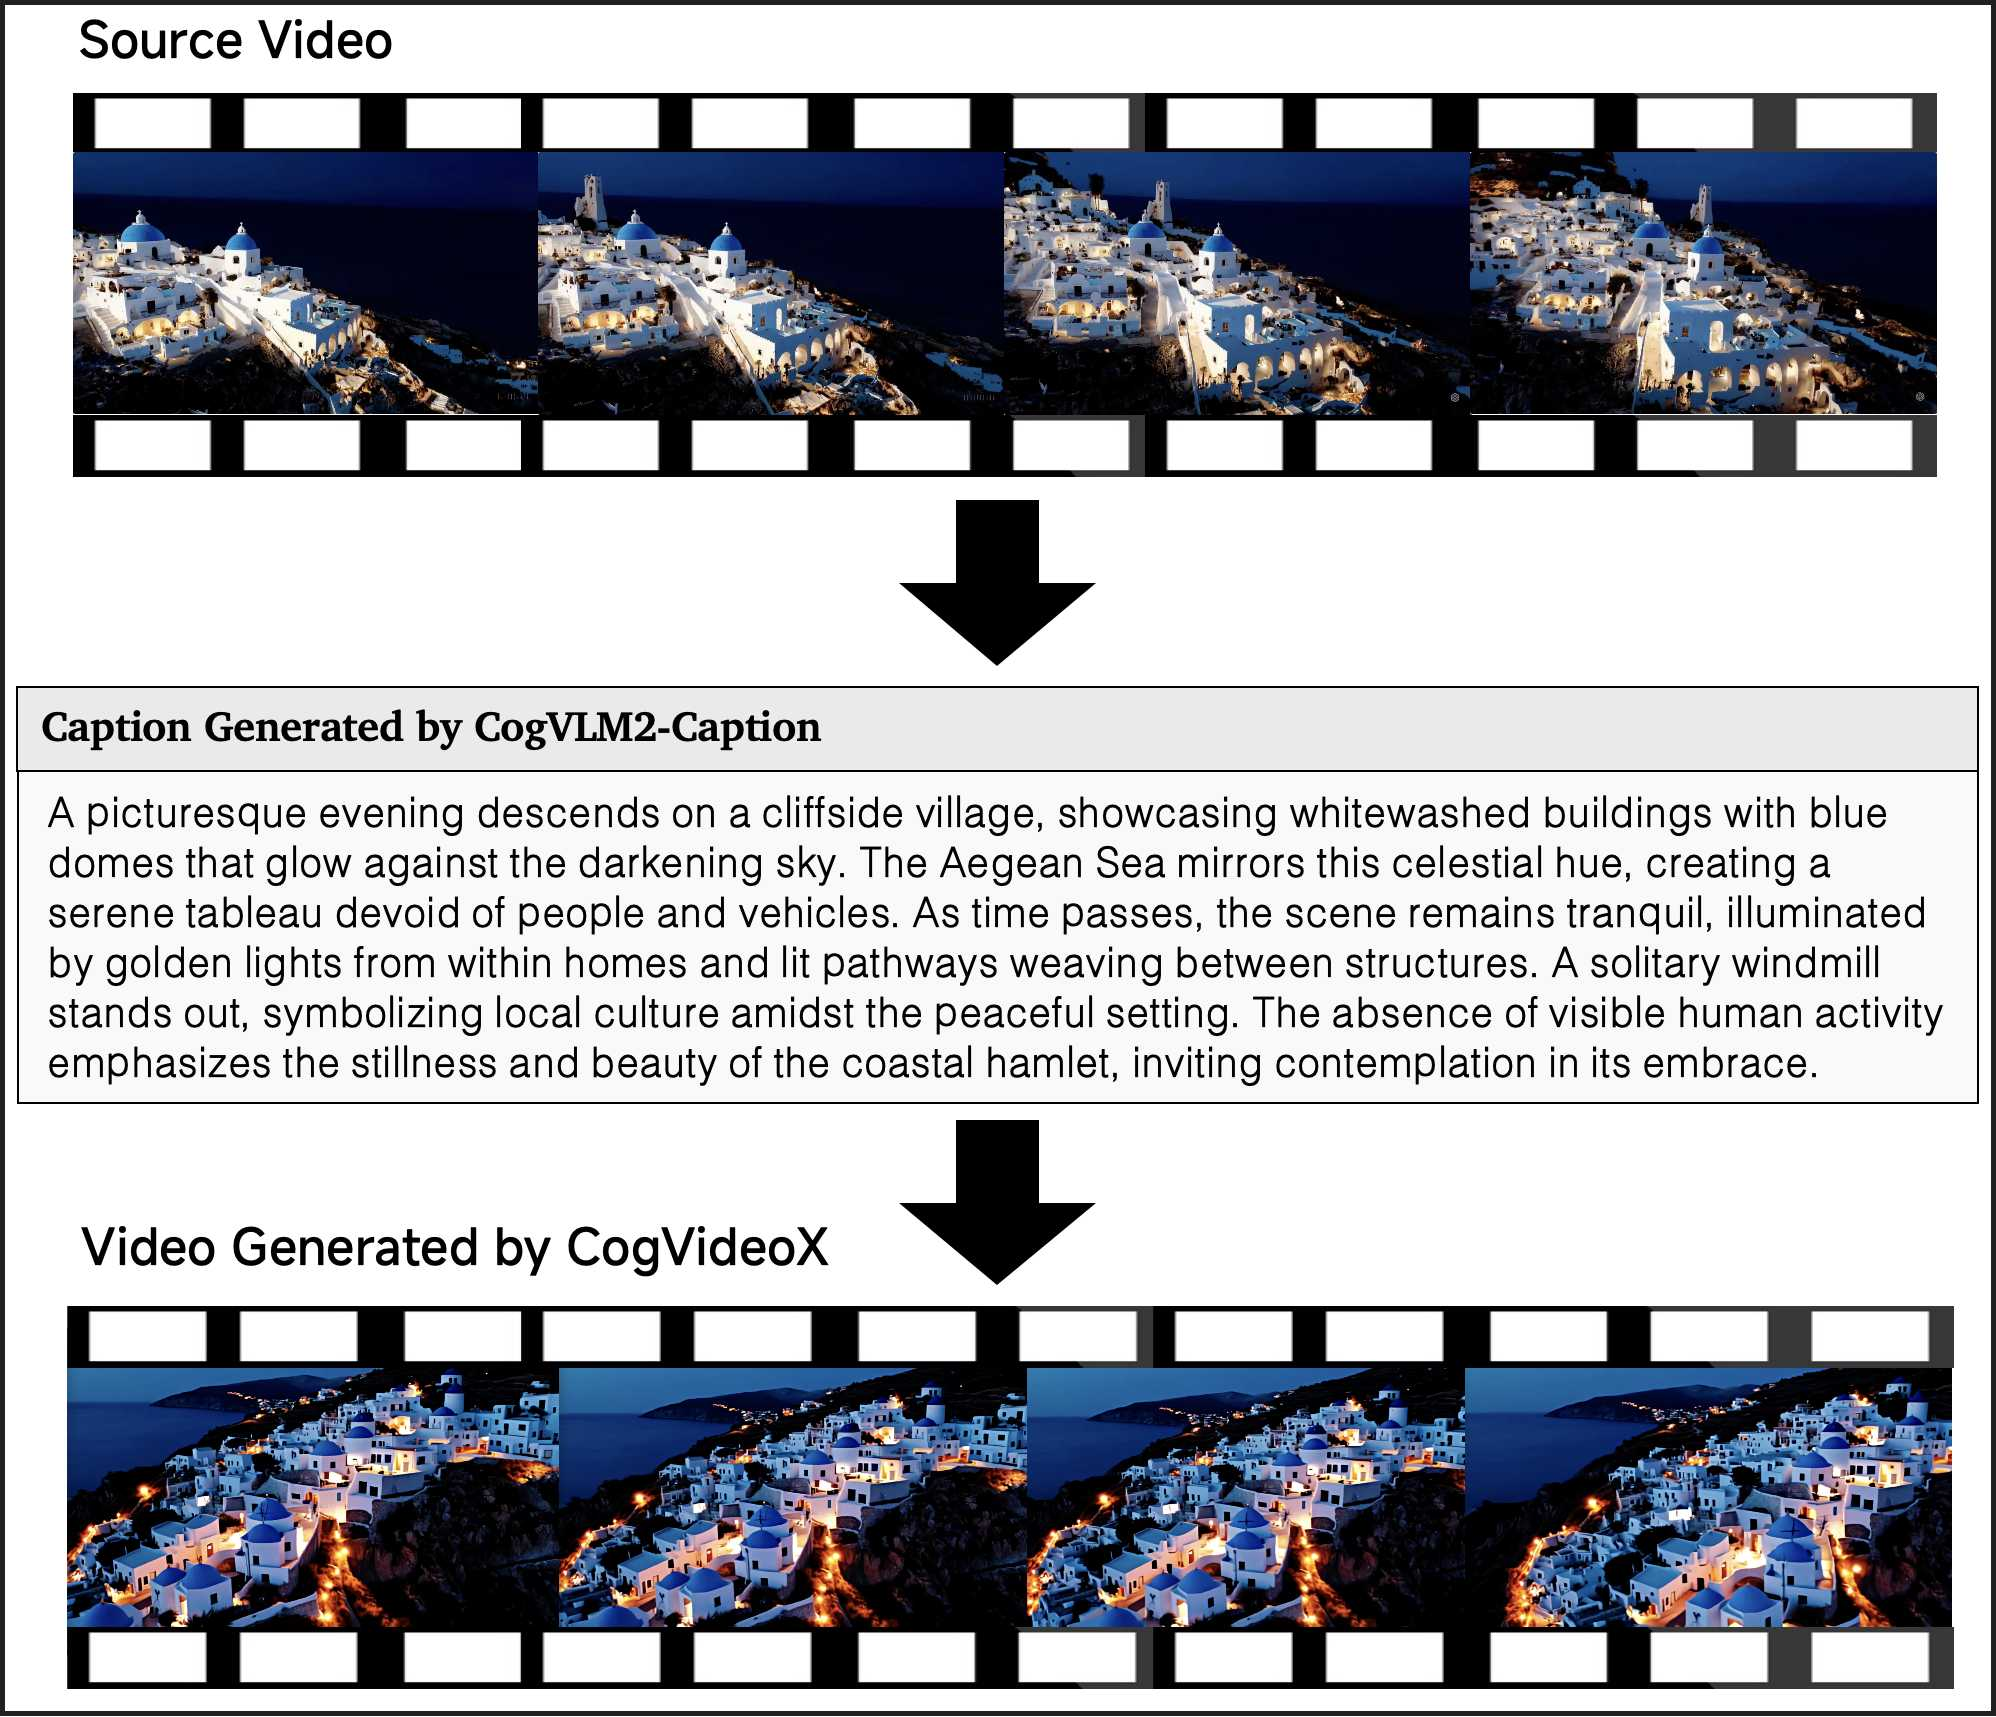
\includegraphics[width=0.9\linewidth]{images/v2v/v2v_2.jpg}
\end{center}
\end{figure}

\begin{figure}[h]
\begin{center}
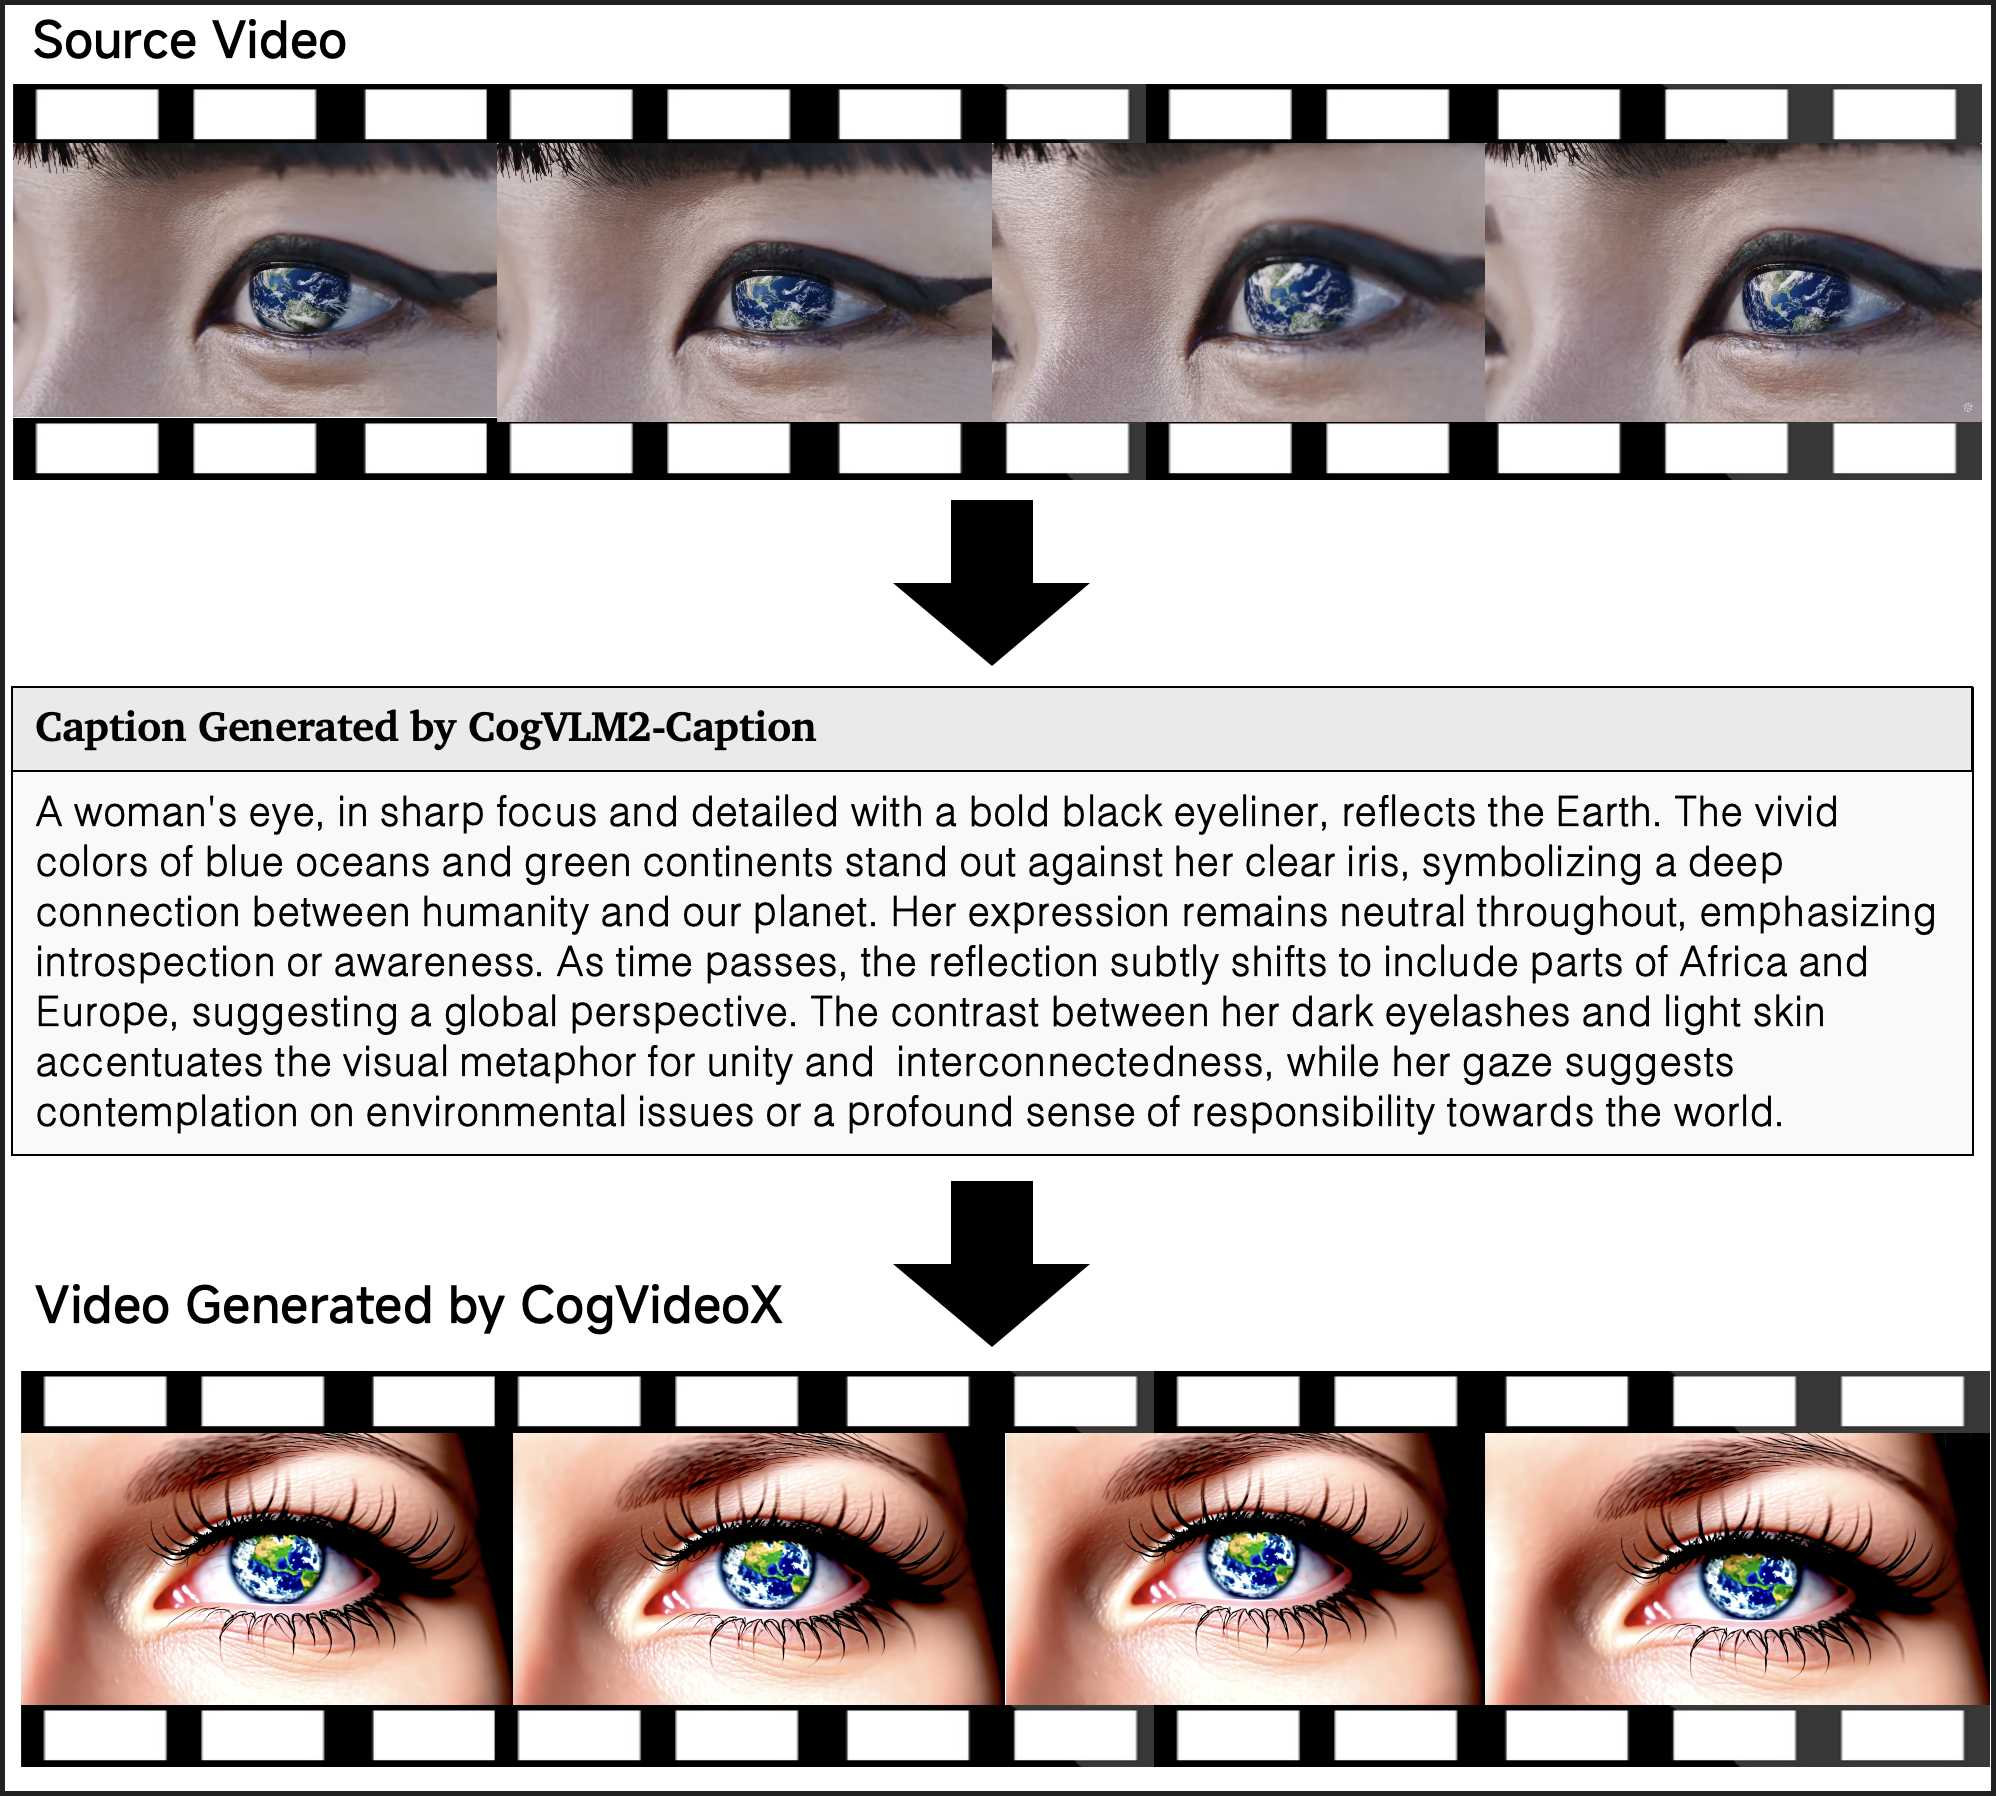
\includegraphics[width=0.9\linewidth]{images/v2v/v2v_3.jpg}
\end{center}
\end{figure}


\begin{table}[!ht]
\centering
\label{sample-table}
\small
\vspace{-5pt}
\caption{Human evaluation between CogVideoX and Kling.}
\label{table:human_eva}
\resizebox{0.75\linewidth}{!}{
    \begin{tabular}{cccccc}
    \toprule
        Model & \Centerstack{Sensory\\Quality} & \Centerstack{Instruction\\Following}&\Centerstack{Physics\\Simulation} & \Centerstack{Cover\\Quality} & 
        \Centerstack{Total\\Score} \\ 
        \midrule
        Kling & 0.638 & 0.367 & 0.561 & 0.668 & 2.17 \\
        \midrule
         {\bf CogVideoX-5B} & {\bf 0.722} & {\bf 0.495} & {\bf 0.667} & {\bf 0.712} & {\bf 2.74}  \\
        \bottomrule
    \end{tabular}
}
\vspace{-3mm}
\end{table}
\vspace{-0.5em}
\section{Data Filtering Details}
\label{ap:data_filtering_details}
In order to obtain high-quality training data, we designed a set of negative labels to filter out low-quality data. Figure \ref{fig:exp_filter} presents our negative labels along with sample videos for each label.In \cref{tab:classifier}, we present the accuracy and recall of our classifier, trained based on video-llama, on the test set (10\% randomly labeled data).

\begin{table}[h]
    \centering
    \caption{Summary of Classifiers Performance on the Test Set. TP: True Positive, FP: False Positive, TN: True Negative, FN: False Negative.}
        \begin{tabular}{cccccc}
        \toprule
        Classifier & TP  & FP & TN & FN & Test Acc \\
        \midrule
        Classifier - Editing & 0.81 & 0.02 & 0.09 &  0.08 & 0.91 \\ 
        Classifier - Static & 0.48 & 0.04 & 0.44 & 0.04 & 0.92 \\
        Classifier - Lecture & 0.52 & 0.00 & 0.47 & 0.01 & 0.99 \\
        Classifier - Text & 0.60 & 0.03 & 0.36 & 0.02 & 0.96 \\
        Classifier - Screenshot & 0.61 & 0.01 & 0.37 & 0.01 & 0.98 \\
        Classifier - Low Quality & 0.80 & 0.02 & 0.09 & 0.09 & 0.89 \\
        \bottomrule
        \end{tabular}
    \label{tab:classifier}
\end{table}

\begin{figure}[ht]
\begin{center}
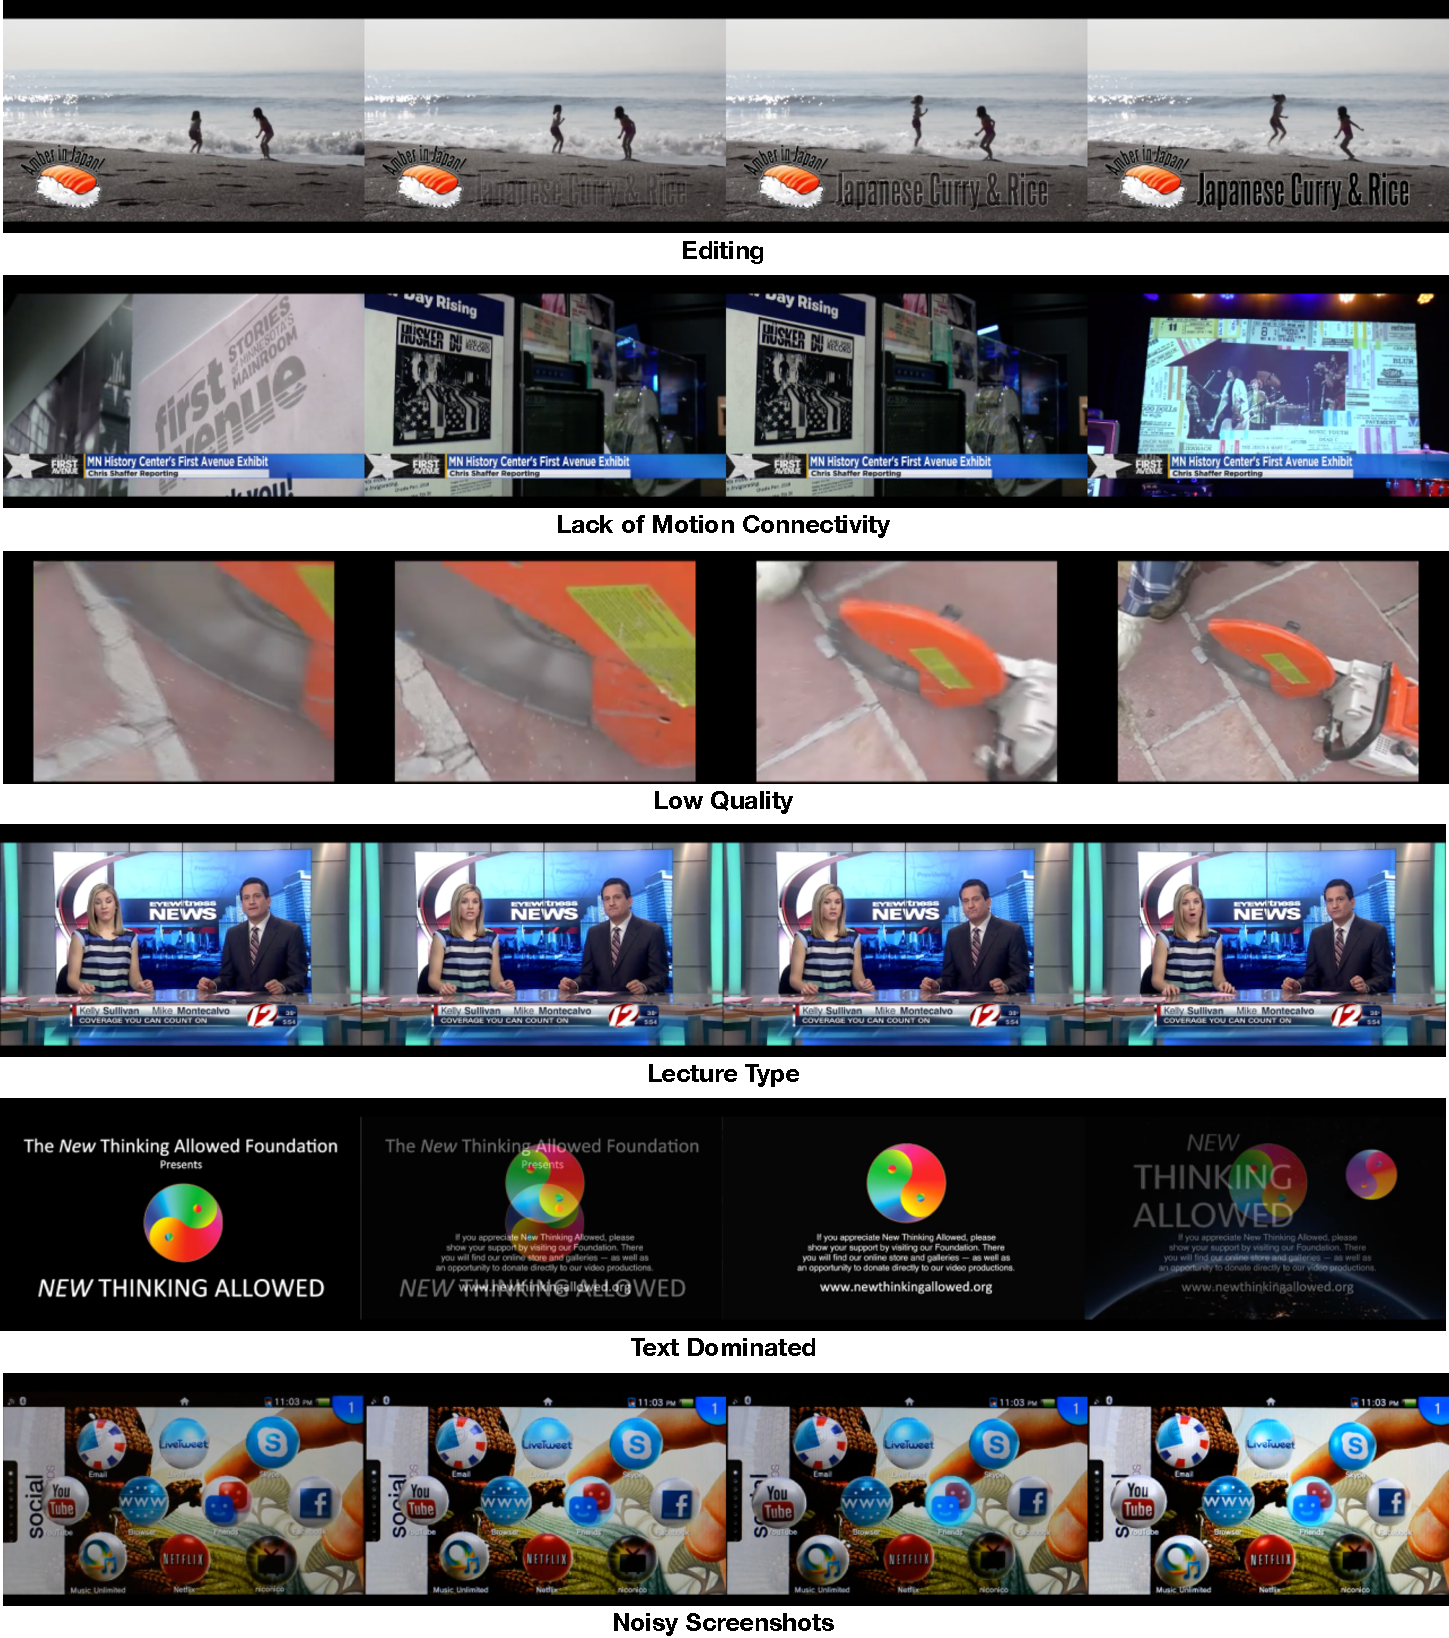
\includegraphics[width=0.9\linewidth]{images/data_filter/VideoFilter.pdf}
\end{center}
\vspace{-0.5em}
\caption{Examples of negative labels for video filtering.}
\label{fig:exp_filter}

\end{figure}



\end{document}